%% This is the ctufit-thesis example file. It is used to produce theses
%% for submission to Czech Technical University, Faculty of Information Technology.
%%
%% This is version 1.6.0, built 18. 9. 2025.
%% 
%% Get the newest version from
%% https://gitlab.fit.cvut.cz/theses-templates/FITthesis-LaTeX
%%
%%
%% Copyright 2024, Tomas Novacek
%% Copyright 2021, Eliska Sestakova and Ondrej Guth
%%
%% This work may be distributed and/or modified under the
%% conditions of the LaTeX Project Public License, either version 1.3
%% of this license or (at your option) any later version.
%% The latest version of this license is in
%%  https://www.latex-project.org/lppl.txt
%% and version 1.3 or later is part of all distributions of LaTeX
%% version 2005/12/01 or later.
%%
%% This work has the LPPL maintenance status `maintained'.
%%
%% The current maintainer of this work is Tomas Novacek (novacto3@fit.cvut.cz).
%% Alternatively, submit bug reports to the tracker at
%% https://gitlab.fit.cvut.cz/theses-templates/FITthesis-LaTeX/issues
%%
%%

% arara: xelatex
% arara: biber
% arara: xelatex
% arara: xelatex

%%%%%%%%%%%%%%%%%%%%%%%%%%%%%%%%%%%%%%%%%
% CLASS OPTIONS
% language: czech/english/slovak
% thesis type: bachelor/master/dissertation/doctoral-report
% electronic (oneside) or printed (twoside), twoside is default
% paragraph - if passed, this optional argument sets paragraphs as the deepest level of headers, styles it, numbers it and adds it to Table of Content. Use with care! Normally, it is considered unwise to use it, since it is too deep.
% colour: bw for black&white OR no option for default colour scheme
%%%%%%%%%%%%%%%%%%%%%%%%%%%%%%%%%%%%%%%%%
\documentclass[english,master,oneside]{ctufit-thesis}

%%%%%%%%%%%%%%%%%%%%%%%%%%%%%%%%%%
% FILL IN THIS INFORMATION
%%%%%%%%%%%%%%%%%%%%%%%%%%%%%%%%%%
\ctufittitle{Detection of Inflammatory Cells in Histological Images Using Computer Vision and Deep Learning Methods} % replace with the title of your thesis
\ctufitauthorfull{Bc. Štěpán Tupý} % replace with your full name (first name(s) and then family name(s) / surname(s)) including academic degrees
\ctufitauthorsurnames{Tupý} % replace with your surname(s) / family name(s)
\ctufitauthorgivennames{Štěpán} % replace with your first name(s) / given name(s)
\ctufitsupervisor{prof. Ing. Vanda Benešová, CSc.} % replace with name of your supervisor/advisor (include academic degrees)
\ctufitdepartment{Department of Applied Mathematics} % replace with the department of your defence
\ctufitprogram{Informatics} % replace with your study program
\ctufitspecialisation{Knowledge Engineering} % replace with your specialisation
\ctufityear{2026} % replace with the year of your defence
\ctufitdeclarationplace{Prague} % replace with the place where you sign the declaration
\ctufitdeclarationdate{February 15, 2026} % replace with the date of signature of the declaration
\ctufitabstractCZE{Pro prevenci selhání transplantované ledviny je nutné monitorovat její stav, a v případě podezření na odmítnutí provést biopsii. Zánětlivé buňky hrají zásadní roli při odmítnutí transplantátu a jejich přítomnost a rozsah je třeba při posuzování biopsie vyhodnotit, což je časově náročný proces s omezenou reprodukovatelností. Tato práce se zaměřuje na automatizaci tohoto vyhodnocení a navrhuje přístup založený na hlubokém učení pro detekci mononukleárních zánětlivých buněk v biopsiích transplantovaných ledvin, včetně jejich klasifikace na lymfocyty a monocyty. Anotovaný dataset poskytnutý v rámci MONKEY Challenge, skládající se z 81 histologických snímků, byl využit k trénování konvoluční sítě pro detekci objektů YOLO11 pomocí bounding boxů vygenerovaných na základě poskytnutých bodových anotací. Model byl vyhodnocen v rámci MONKEY Challenge, kde dosáhl konkurenceschopných výsledků ve srovnání s ostatními účastníky. Výsledky prokazují proveditelnost automatizace této detekce a navržený model by mohl asistovat patologům při posuzování biopsií transplantovaných ledvin.}
\ctufitabstractENG{To prevent kidney transplant failure, the condition of the organ must be monitored, and a biopsy is performed when rejection is suspected. Inflammatory cells play an essential role in transplant rejection and their presence and extent need to be evaluated during the assessment of the biopsy, a process that is time-consuming and has limited reproducibility. This thesis focuses on automating this assessment and proposes a deep learning approach for the detection of mononuclear inflammatory cells in kidney transplant biopsies, including their classification into lymphocytes and monocytes. An annotated dataset provided by the MONKEY Challenge, consisting of 81 histological images, was utilized to train the convolutional object detection network YOLO11 using bounding boxes generated from provided dot annotations. The model was evaluated in the MONKEY Challenge and achieved competitive performance among other submissions. The results demonstrate the feasibility of automating the detection process and the proposed model could assist pathologists during kidney transplant biopsy assessment.}
\ctufitkeywordsCZE{digitální histopatologie, zpracování lékařských snímků, počítačové vidění, detekce objektů, hluboké učení, konvoluční neuronové sítě}
\ctufitkeywordsENG{digital histopathology, medical image processing, computer vision, object detection, deep learning, convolutional neural networks}
%%%%%%%%%%%%%%%%%%%%%%%%%%%%%%%%%%
% END FILL IN
%%%%%%%%%%%%%%%%%%%%%%%%%%%%%%%%%%

%%%%%%%%%%%%%%%%%%%%%%%%%%%%%%%%%%
% CUSTOMIZATION of this template
% Skip this part or alter it if you know what you are doing.
%%%%%%%%%%%%%%%%%%%%%%%%%%%%%%%%%%

\RequirePackage{iftex}[2020/03/06]
\iftutex % XeLaTeX and LuaLaTeX
    \RequirePackage{ellipsis}[2020/05/22] %ellipsis workaround for XeLaTeX
\else
    \errmessage{Only compilation with XeLaTeX or LuaLaTeX is allowed}
    \stop
\fi

% hyperlinks
\hypersetup{
    pdfpagelayout=TwoPageRight,
    colorlinks=false,
    allcolors=decoration,
    pdfborder={0 0 0.1}
}

% uncomment the following to hide all hyperlinks
\hypersetup{hidelinks}

% uncomment the following to change the colour of all hyperlinks to CTU blue
%\hypersetup{allbordercolors=decoration}

\RequirePackage{pdfpages}[2020/01/28]

%%%%%%%%%%%%%%%%%%%%%%%%%%%%%%%%%%
% CUSTOMIZATION of this template END
%%%%%%%%%%%%%%%%%%%%%%%%%%%%%%%%%%


%%%%%%%%%%%%%%%%%%%%%%
% PACKAGES SETTINGS
% You may choose to modify this part.
%%%%%%%%%%%%%%%%%%%%%%
\usepackage{dirtree}
\usepackage{lipsum,tikz}
\usepackage[style=iso-numeric]{biblatex}
\addbibresource{text/bib-database.bib}
\usepackage{xurl}
\usepackage{listings} % typesetting of sources
%\usepackage{minted}
\usepackage{csquotes}
\usepackage[ruled, algochapter, linesnumbered]{algorithm2e}
\usepackage{amsmath}
\usepackage{bbm}
\usepackage{booktabs}
\usepackage{makecell}

%%%%%%%%%%%%%%%%%%%%%%
% PACKAGES SETTINGS END
%%%%%%%%%%%%%%%%%%%%%%

\begin{document}
\frontmatter\frontmatterinit % do not remove these two commands

\thispagestyle{empty}\maketitle\thispagestyle{empty}\cleardoublepage % do not remove these four commands

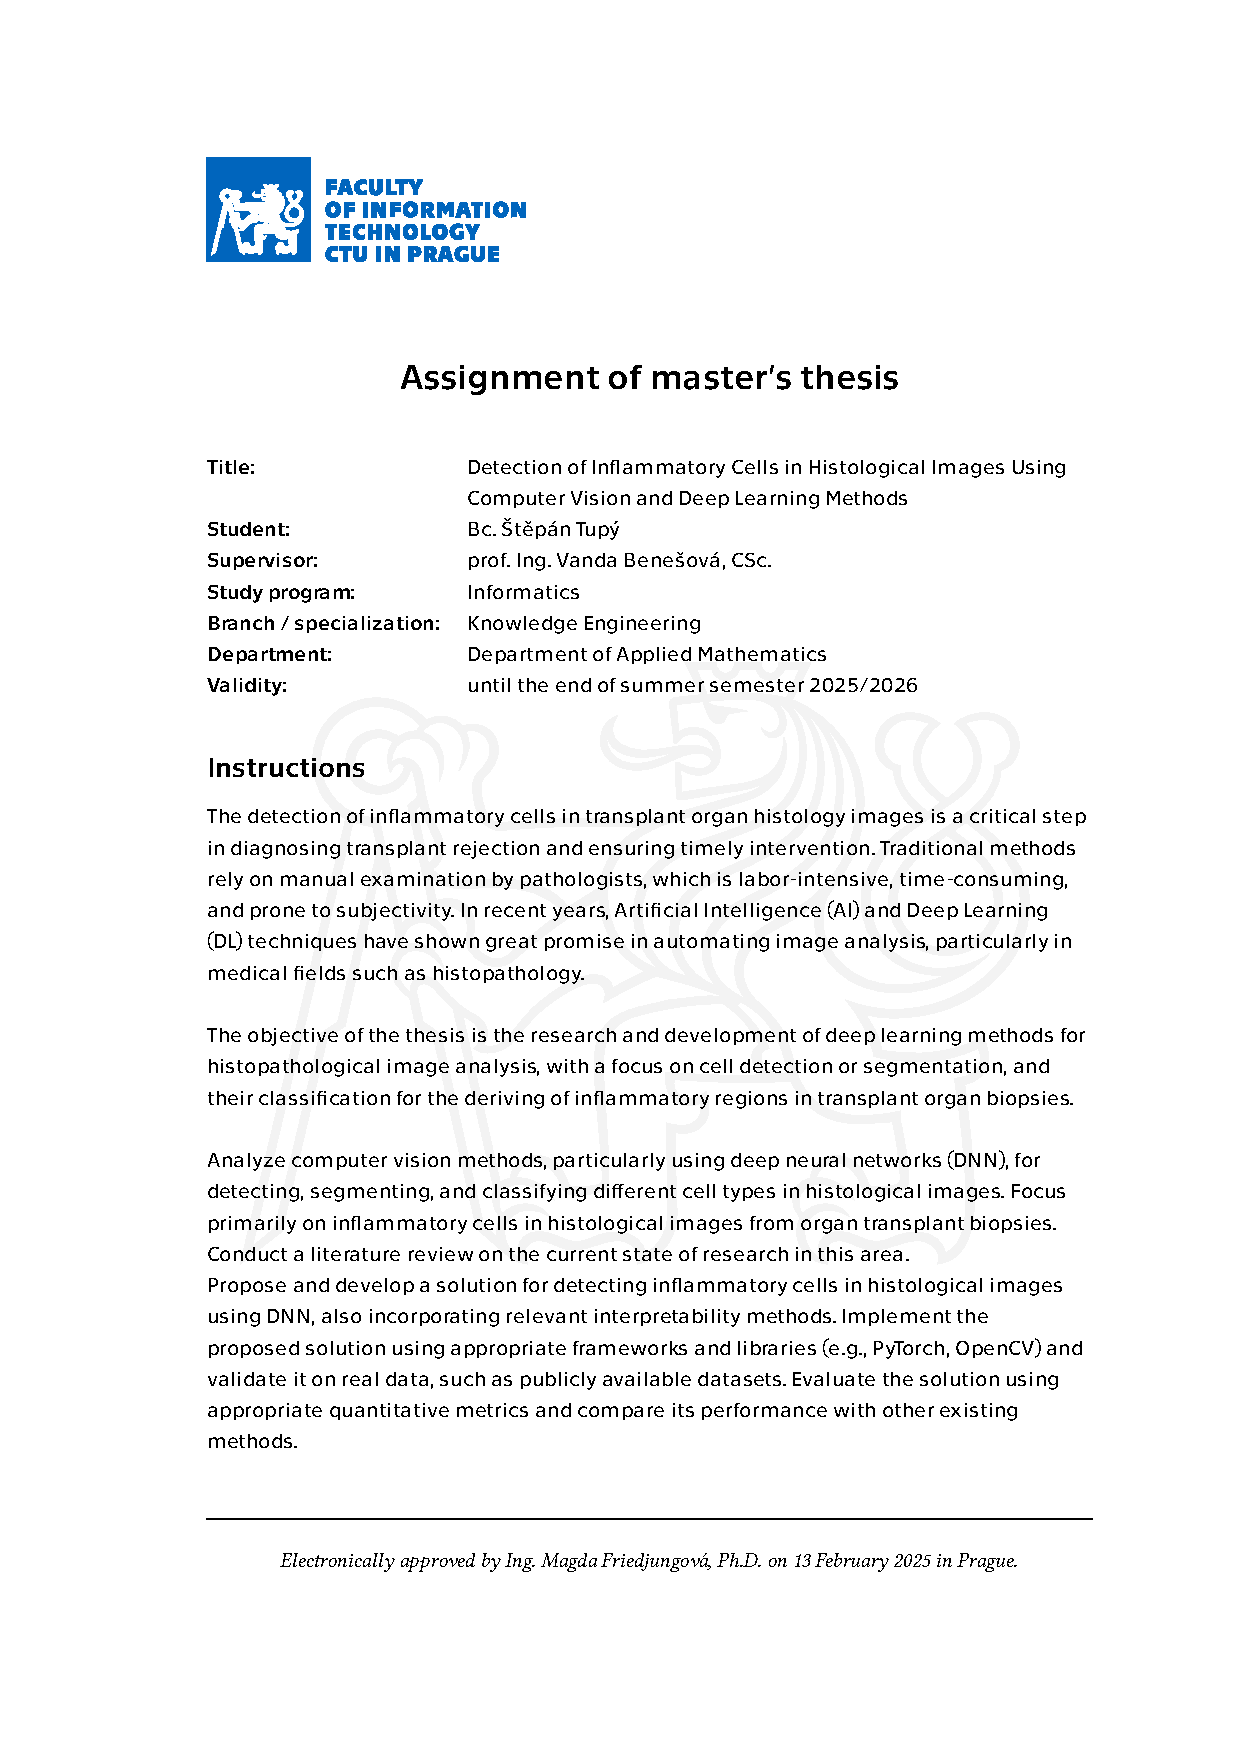
\includepdf[pages={1-}]{tupystep-assignment.pdf} % replace this file with your thesis assignment generated from ProjectsFIT

\imprintpage % do not remove this command
\stopTOCentries

%%%%%%%%%%%%%%%%%%%
% ACKNOWLEDGMENT
% FILL IN / MODIFY
% This is a place to thank people for helping you. It is common to thank your supervisor.
%%%%%%%%%%%%%%%%%%%
\begin{acknowledgmentpage}
	I would like to thank my supervisor prof. Ing. Vanda Benešová, CSc. for her guidance, advice, and frequent consultations. I would also like to thank the organizers of the MONKEY Challenge for creating and providing such a valuable dataset.
\end{acknowledgmentpage}
%%%%%%%%%%%%%%%%%%%
% ACKNOWLEDGMENT END
%%%%%%%%%%%%%%%%%%%


%%%%%%%%%%%%%%%%%%%
% DECLARATION
% FILL IN / MODIFY
%%%%%%%%%%%%%%%%%%%
% INSTRUCTIONS
% ENG: choose one of approved texts of the declaration. DO NOT CREATE YOUR OWN. Find the approved texts at https://courses.fit.cvut.cz/SFE/download/index.html#_documents (document Declaration for FT in English)
% CZE/SLO: Vyberte jedno z fakultou schvalenych prohlaseni. NEVKLADEJTE VLASTNI TEXT. Schvalena prohlaseni najdete zde: https://courses.fit.cvut.cz/SZZ/dokumenty/index.html#_dokumenty (prohlášení do ZP)
\begin{declarationpage}
	I hereby declare that the presented thesis is my own work and that I have cited all sources of information in accordance with the Guideline for adhering to ethical principles when elaborating an academic final thesis. I declare that I have used AI tools during the preparation and writing of my thesis. I have verified the generated content. I confirm that I am aware that I am fully responsible for the content of the thesis.
    
    I acknowledge that my thesis is subject to the rights and obligations stipulated by the Act No. 121/2000 Coll., the Copyright Act, as amended, in particular the fact that the Czech Technical University in Prague has the right to conclude a license agreement on the utilization of this thesis as a school work pursuant of Section 60 (1) of the Act.
\end{declarationpage}
%%%%%%%%%%%%%%%%%%%
% DECLARATION END
%%%%%%%%%%%%%%%%%%%

% Use one of the two following commands. The first prints abstracts+keywords on two pages, the second puts them on one page (if possible). \printonepageabstract can also accept optional argument that specifies a vertical space before both abstracts (the default is 18 mm).
% \printtwopageabstract
\printonepageabstract[0mm]

\tableofcontents % do not remove this command
%%%%%%%%%%%%%%%%%%%%%%
% list of other contents: figures, tables, code listings, algorithms, etc.
% add/remove commands accordingly
%%%%%%%%%%%%%%%%%%%%%%
\listoffigures % list of figures
\begingroup
\let\clearpage\relax
\listoftables % list of tables. Remove if you do not have any.
% \thectufitlistingscommand{} % list of code listings. Remove if you do not have any.
\thectufitlistofalgorithmscommand{} % list of algorithm pseudocodes defined using the algorithm package.
\endgroup
%%%%%%%%%%%%%%%%%%%%%%
% list of other contents END
%%%%%%%%%%%%%%%%%%%%%%

%%%%%%%%%%%%%%%%%%%
% ABBREVIATIONS
% FILL IN / MODIFY
% OR REMOVE ENTIRELY
% List the abbreviations in lexicography order.
%%%%%%%%%%%%%%%%%%%
\chapter{\thectufitabbreviationlabel}

\begin{tabular}{rl}
    AP    & Average Precision                              \\
	AUC   & Area Under the Curve                           \\
    BF    & Boundary F1-Score                              \\
    CNN   & Convolutional Neural Network                   \\
    DETR  & Detection Transformer                          \\
	FPR   & False Positive Rate                            \\
    FROC  & Free Response Operating Characteristic         \\
    GAN   & Generative Adversarial Network                 \\
    GELU  & Gaussian Error Linear Unit                     \\
    IHC   & Immunohistochemistry                           \\
    IoU   & Intersection over Union                        \\
    LReLU & Leaky ReLU                                     \\
	mAP   & Mean Average Precision                         \\
    NMS   & Non-Maximum Suppression                        \\
    NPV   & Negative Predictive Value                      \\
    PAS   & Periodic Acid-Schiff                           \\
    PReLU & Parametric ReLU                                \\
    PR    & Precision-Recall                               \\
    R-CNN & Regions with CNN features                      \\
    ReLU  & Rectified Linear Unit                          \\
    ROC   & Receiver Operating Characteristic              \\
    ROI   & Region of Interest                             \\
    RPN   & Region Proposal Network                        \\
    SAM 2 & Segment Anything Model 2                       \\
    SGD   & Stochastic Gradient Descent                    \\
    SVM   & Support Vector Machine                         \\
	TNR   & True Negative Rate                             \\
    TPR   & True Positive Rate                             \\
    WSI   & Whole-Slide Image                              \\
    YOLO  & You Only Look Once                             \\
\end{tabular}
%%%%%%%%%%%%%%%%%%%
% ABBREVIATIONS END
%%%%%%%%%%%%%%%%%%%
\resumeTOCentries
\mainmatter\mainmatterinit % do not remove these two commands
%%%%%%%%%%%%%%%%%%%
% THE THESIS
% MODIFY ANYTHING BELOW THIS LINE
%%%%%%%%%%%%%%%%%%%

% Do not forget to include Introduction
%---------------------------------------------------------------
\chapter{Introduction}
% uncomment the following line to create an unnumbered chapter
%\chapter*{Introduction}\addcontentsline{toc}{chapter}{Introduction}\markboth{Introduction}{Introduction}
%---------------------------------------------------------------
\setcounter{page}{1}
Medical imaging plays a crucial role in modern healthcare, as physicians and specialists often rely on medical images to make diagnoses and develop new treatments. Recent advances in image acquisition and reconstruction technologies have enabled the collection of large volumes of high-resolution radiological and microscopic images. Their interpretation requires expertise and diligence and is often tedious and time-consuming. Therefore, accurate automated analysis is desirable. It can reduce the burden on pathologists and radiologists and provide precise diagnoses and earlier detections while reducing human variability. Such automation can also expedite surgical care in low-resource environments where specialized physicians are not readily available.~\cite{Aljuaid2022, Lindroth2024}

Computer vision enables the automation of many tasks that require the interpretation of visual information. In recent years, the number of publications that apply computer vision techniques to medical images has increased significantly. Areas such as radiology, pathology, ophthalmology, and dermatology have received substantial attention due to the visual pattern recognition nature of diagnostic tasks in these specialties and the growing availability of structured imaging data. The performance of computer vision methods, particularly deep learning, has often been shown to match or even surpass the level of expert physicians in the analysis of medical images.~\cite{Esteva2021}

Another area that benefits from the deployment of computer vision is histopathology, which is concerned with the analysis of tissue samples to identify patterns and establish diagnoses. Histopathology produces extremely large high-resolution images that cannot be manually processed by pathologists in their entirety. Computer vision and deep learning can be implemented to analyze histological images, automating the extraction and quantification of relevant biological and clinical features.~\cite{Moscalu2023}

\section{Automated Assessment of Kidney Transplant Biopsies}
The application of computer vision methods to histopathology is the objective of my thesis. I develop a deep learning model for the detection of inflammatory cells in kidney transplant biopsies using annotated histological data provided by the MONKEY Challenge~\cite{Studer2024}. The data, collected during routine diagnostics at different institutions, consists of Periodic Acid-Schiff (PAS) stained histology slides digitized using a Whole-Slide Image (WSI) scanner. Figure~\ref{fig:monkey} shows a sample WSI with annotations in a Region of Interest (ROI). The MONKEY Challenge is focused on developing machine learning algorithms for the detection of mononuclear inflammatory cells in the PAS-stained WSIs, followed by their classification into lymphocytes and monocytes.

\begin{figure}[!b]
    \centering
    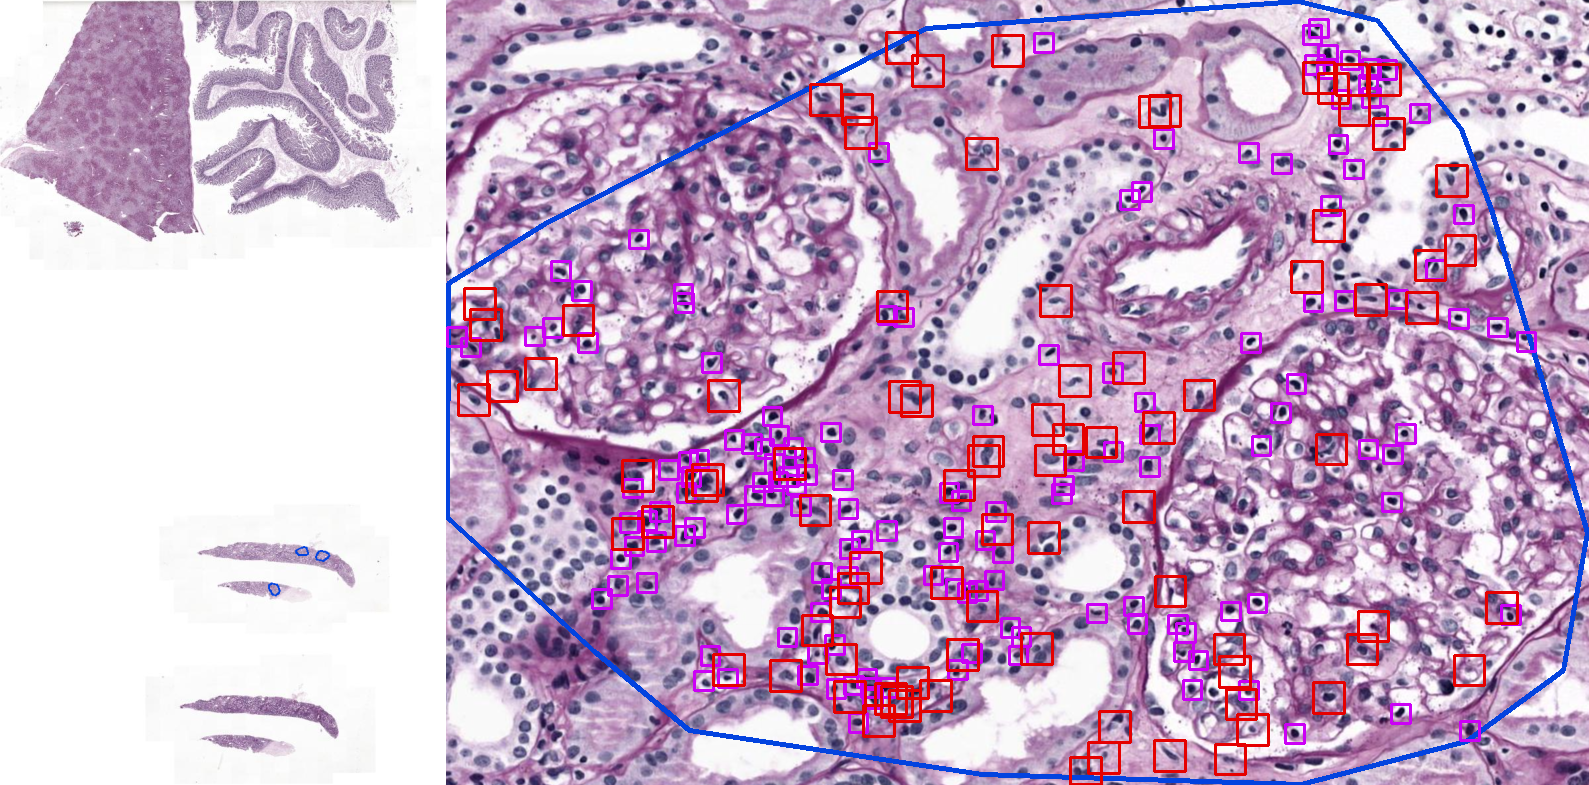
\includegraphics[width=\linewidth]{images/sample_wsi.png}
    \caption{Left: PAS-stained WSI showing three ROIs marked in blue. Right: magnified view of one ROI with bounding boxes drawn around provided dot annotations for lymphocytes (purple) and monocytes (red).}
    \label{fig:monkey}
\end{figure}

Kidney transplantation is the preferred treatment for patients with end-stage kidney disease. To prevent transplant organ failure, it is necessary to monitor recovery progress and detect any signs of potential complications, such as organ rejection. When acute or chronic rejection is suspected, a kidney biopsy is performed to assess the condition of the donor organ and guide the treatment strategy to ensure its longevity. The Banff classification~\cite{Roufosse2018} is the standard for histopathological assessment of transplant kidney biopsies. It consists of 17 Banff lesion scores, ten of which focus on the presence and extent of inflammatory cells in different kidney compartments. The inflammatory cells, also known as leukocytes or white blood cells, are the major cellular component of the immune response and play an essential role in transplant rejection. 

Most Banff lesion scores are graded semi-quantitatively as mild, moderate, or severe based on the number of inflammatory cells within the corresponding kidney compartment. The assessment of the individual scores is crucial and must be objective and consistent, as the results determine the diagnosis and subsequent treatment decisions. However, Banff scoring has mediocre reproducibility and is time-consuming in daily practice. Automated biopsy assessment could reduce the workload of pathologists while increasing the scoring consistency and efficiency.

The most common type of inflammatory cells scored for transplant organ rejection are mononuclear leukocytes, which can be further differentiated into lymphocytes and monocytes. Pathologists do not make this distinction during Banff scoring, but research suggests that the subtypes may play different roles in transplant rejection. Monocytes are the largest cell type in the blood, with a diameter of 15--22 \textmu m, while lymphocytes are smaller, with a diameter of approximately 7 \textmu m. Pathologists can differentiate between these cells based on certain morphological features, but it remains challenging to do so with certainty. Immunohistochemistry (IHC) staining can be applied to better distinguish the cells and was used to guide the provided annotations on the PAS slides.

\paragraph{Deep learning approach} I propose and develop a deep learning model for the automated assessment of kidney transplant biopsies. I frame the task of evaluating the presence and extent of mononuclear inflammatory cells as an object detection problem and train the convolutional neural network YOLO11~\cite{Jocher2024} to detect and classify lymphocytes and monocytes in PAS-stained histological WSIs of transplant kidney biopsies. To enable training on the provided data, I first divide the high-resolution WSIs into patches of fixed size and convert the dot annotations into bounding box labels. I then evaluate the performance of models trained across different training setups and compare the best-performing version with other solutions submitted to the MONKEY Challenge.



\chapter{Computer Vision}
Computer vision is a field of artificial intelligence that focuses on the high-level computer understanding and interpretation of visual information from images and videos. Its main goal is to extract useful information from visual data and use it for decision-making. Reliable interpretation of real-world images has been one of the most complex challenges in computer science, motivating the development of many computer vision methods. The field started in the 1960s with image processing experiments such as edge detection and pattern recognition~\cite{Shapiro2020}. Since then, it has gradually evolved to rely on deep learning models and large datasets.

These advancements have allowed computer vision to be applied in many aspects of daily life and industry. It enables the automation of tasks that require visual understanding, improving both efficiency and consistency. It is used in many areas, such as quality control in manufacturing~\cite{Islam2024}, navigation in autonomous vehicles~\cite{Horgan2015}, and surveillance~\cite{Cazzato2020}. In all of these cases, computer vision replaces or assists human visual inspection, making complex processes faster and more reliable.

\paragraph{Medical imaging} Computer vision also plays an increasingly important role in healthcare, where image interpretation is essential for the correct diagnosis of many diseases. Computer vision methods have demonstrated impressive performance in the analysis of medical images and have been shown to be comparable in ability to humans. Given sufficient data, their accuracy can even surpass the level of expert physicians~\cite{Esteva2021}.

However, major challenges remain in applying computer vision to medical image analysis. Deep learning, in particular, typically requires large amounts of data to achieve good performance and generalization, while high-quality annotated medical image datasets are scarce. Most publicly available datasets consist of a limited number of patients because data collection requires expert clinicians to provide labels and interpretations, which is expensive and time-consuming. Furthermore, data collection involving human subjects requires ensuring privacy and patient safety.

This causes large medical imaging datasets to be rare and often difficult to access, making transfer learning, in which a model is pre-trained on a large dataset before being fine-tuned on the dataset of interest, critical for progress~\cite{Esteva2021}. Another significant issue in biomedical datasets is class imbalance. In imbalanced datasets, the distribution of samples across classes is highly uneven, which can negatively affect model performance and generalization to new data. Data augmentation can be used to mitigate this problem by effectively increasing the number of samples.~\cite{Aljuaid2022, Lindroth2024}


\section{Computer Vision Tasks}
Computer vision is a broad field, and its problems are commonly organized into distinct tasks, each representing a specific type of visual objective. They focus on a different level of image interpretation and serve as the basis for more advanced applications. This organization clarifies the expected outputs and enables comparison of different approaches.

While there are many different tasks, the following sections will focus on the ones that are most relevant to medical image analysis and my thesis: \textbf{image classification}, \textbf{object detection}, and \textbf{image segmentation}. A basic comparison of these tasks is shown in Figure~\ref{fig:tasks}. Their definitions determine the requirements for model outputs and their characteristics influence model architecture and the features that must be learned.

\begin{figure}[b]
    \centering
    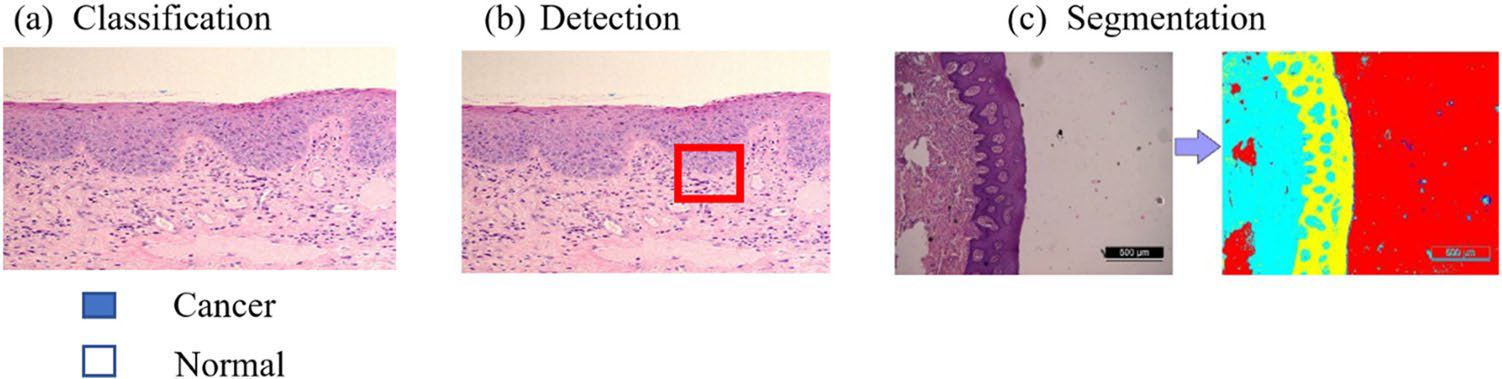
\includegraphics[width=\linewidth]{images/cv_tasks.png}
    \caption{Conceptual comparison of computer vision tasks.~\cite{Aljuaid2022}}
    \label{fig:tasks}
\end{figure}

\paragraph{Evaluation} Once a computer vision model is trained, its output must be evaluated using performance metrics to ensure that the results are reliable and meaningful. This is even more important in medical applications, where incorrect output could cause harm to patients. Metrics indicate how well the model can generalize to new data and make accurate predictions, and they aid in comparing different models or configurations to identify the best performing ones~\cite{Terven2025}. Evaluation requires metrics that reflect the specific challenges of the task the model performs because different objectives require different evaluation strategies. Image-level decisions are measured with global metrics, while tasks that involve locating or segmenting objects need metrics that assess spatial precision. Using metrics suited to each task ensures that performance is measured accurately and results can be interpreted correctly.


\section{Image Classification}
Image classification involves assigning labels from a predefined set of classes to images based on their content. It is a fundamental task in computer vision because it allows systems to recognize patterns and features at the global level. Classification models aim to learn discriminative representations that can distinguish between categories, even when there are variations in lighting, orientation, or background. It plays an important role in many systems where identifying the overall type of image is sufficient.

\paragraph{ImageNet} Crucial for the advancement of deep learning in image classification has been the ImageNet dataset~\cite{Deng2009, Russakovsky2015}, which contains more than 14 million labeled images organized by the semantic hierarchy of their labels. The complete dataset, called ImageNet-21K, covers more than 21,000 categories, providing broad visual coverage of many different objects and scenes. Its subset of around 1.4 million images, ImageNet-1K, includes 1,000 commonly used categories and serves as a standard benchmark. By providing such a large and diverse set of labeled images, ImageNet enabled deep learning models to achieve high accuracies, and many are pre-trained on this dataset before being fine-tuned for specific tasks. It remains a central benchmark and training resource in computer vision.

\paragraph{Applications in medicine} In medical imaging, classification is used to distinguish between healthy and pathological images. It can be used to improve diagnostic accuracy by automatically detecting and classifying abnormalities such as tumors, fractures, and pathological lesions in various types of scans~\cite{Terven2025}. Because it provides a broad, easily interpretable decision, classification often serves as the first step in medical image analysis pipelines. For example, Brinker et al.~\cite{Brinker2019} trained a deep convolutional neural network to classify suspicious skin lesions as either melanoma or benign nevi. Their model managed to outperform physicians at all levels of expertise within dermatology.

\subsection{Performance Metrics}\label{sec:class}
All classification metrics are calculated based on the \textbf{confusion matrix}, which records the numbers of correctly and incorrectly predicted labels for each class. During binary classification, where models assign only positive or negative labels, the dimensions of the confusion matrix are $2 \times 2$, and it contains the following fields:
\begin{itemize}
    \item \textbf{True Positive (TP):} number of correctly classified positive image instances as positive
    \item \textbf{False Positive (FP):} number of negative image instances incorrectly classified as positive
    \item \textbf{True Negative (TN):} number of correctly classified negative image instances as negative
    \item \textbf{False Negative (FN):} number of positive image instances incorrectly classified as negative
\end{itemize}
Figure~\ref{fig:confusion_matrix} illustrates the structure of the confusion matrix along with associated metrics. The matrix can also be generalized for multiclass classification into $N$ classes by increasing its dimensions to $N \times N$. The diagonal of the matrix then contains the numbers of correctly predicted instance labels for each class. The numbers of incorrect predictions are split between the remaining fields and indicate how much the classes are being interchanged by the model. The following performance metrics for image classification are directly derived from the confusion matrix.~\cite{Terven2025}

\begin{figure}
    \centering
    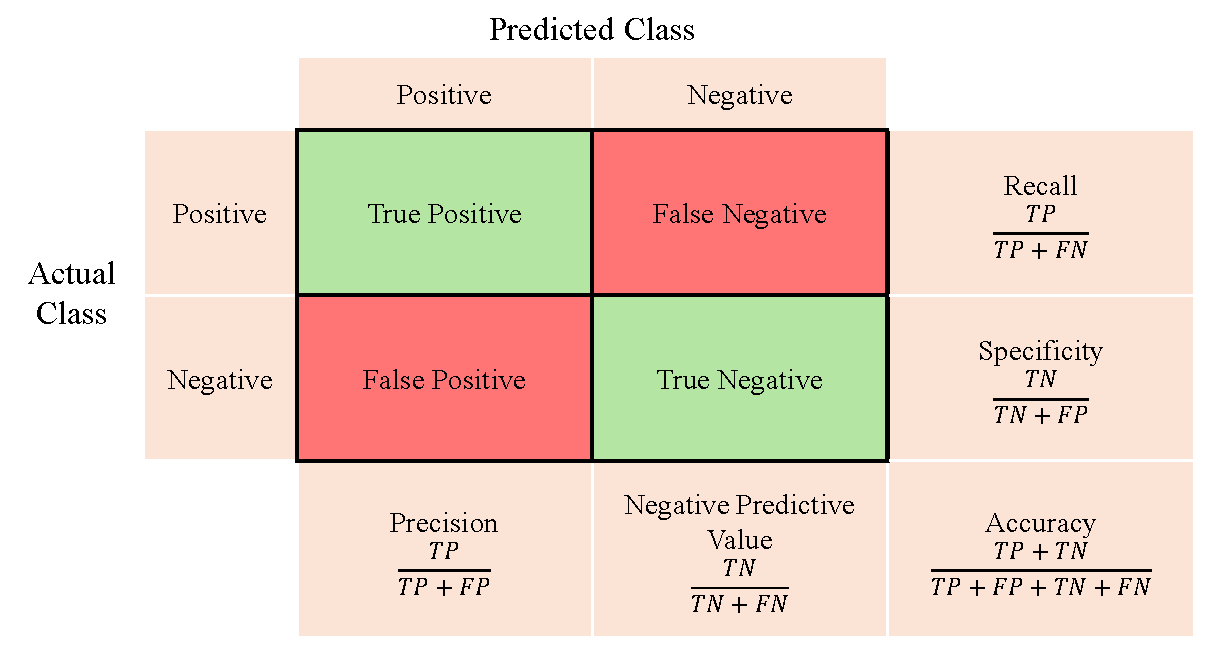
\includegraphics[width=0.9\linewidth]{images/confusion_matrix.pdf}
    \caption{Diagram of the confusion matrix and derived metrics.}
    \label{fig:confusion_matrix}
\end{figure}

\begin{description}
    \item[Accuracy] One of the most widely used classification metrics, defined as the ratio of correctly classified instances. Equation~\ref{eq:acc} defines it for binary classification. Accuracy can be misleading when evaluating severely imbalanced datasets because it does not focus on individual classes. For example, it can still be very high even when the minority class is never predicted and the model is essentially useless.~\cite{Terven2025, Szeliski2022}
    \begin{equation}\label{eq:acc}
        \text{Accuracy} = \frac{\mathrm{TP} + \mathrm{TN}}{\mathrm{TP} + \mathrm{FP} + \mathrm{TN} + \mathrm{FN}}
    \end{equation}

    \item[Precision] Quantifies the ratio of predicted positives that are correctly classified. It does not take false negatives into account at all and is therefore unsuitable in situations where missing positive instances is undesirable. Unlike accuracy, it only focuses on one class, so it can be used to evaluate imbalanced datasets but only when the positive class is the minority. Otherwise, it could be as misleading as accuracy. Precision in multiclass classification is computed for every class separately and can then be averaged.~\cite{Terven2025, Szeliski2022}
    \begin{equation}\label{eq:prec}
        \text{Precision} = \frac{\mathrm{TP}}{\mathrm{TP} + \mathrm{FP}}
    \end{equation}

    \item[Recall (True Positive Rate, TPR)] Usually analyzed together with precision, it measures the ratio of positive instances actually classified as positive. High recall is important in applications where missing positives is costly. Similarly to precision and false negatives, recall does not take false positives into account at all. It can also be used to evaluate imbalanced datasets where the positive class is the minority, and it is calculated per class during multiclass classification.~\cite{Terven2025, Szeliski2022}
    \begin{equation}\label{eq:rec}
        \text{Recall} = \frac{\mathrm{TP}}{\mathrm{TP} + \mathrm{FN}}
    \end{equation}

    \item[F1-Score] Maximizing precision or recall alone can be misleading, because they often act against each other. Predicting more positives usually increases recall but also increases the number of false positives, which in turn decreases precision. In contrast, precision usually increases when predicting fewer positives, which in turn increases the number of false negatives and decreases recall. This is called the \textbf{precision-recall trade-off} and can be addressed by measuring the F1-score defined as the harmonic mean of these two metrics. It ensures that neither precision nor recall is ignored, because it heavily penalizes extreme disparities between them.~\cite{Terven2025, Szeliski2022}
    \begin{equation}\label{eq:f1}
        \text{F1} = 2 \times \frac{\text{Precision} \times \text{Recall}}{\text{Precision} + \text{Recall}}
    \end{equation}

    \item[Negative Predictive Value (NPV)] Quantifies the ratio of negative predictions that are correct. It is the equivalent of precision for negatives as it measures the correctness of negative predictions and limits the number of false negatives.~\cite{Terven2025}
    \begin{equation}\label{eq:npv}
        \mathrm{NPV} = \frac{\mathrm{TN}}{\mathrm{TN} + \mathrm{FN}}
    \end{equation}

    \item[Specificity (True Negative Rate, TNR)] Measures the proportion of negative instances correctly classified as negative. It is the analogy of recall for negative instances and is therefore useful especially when trying to avoid false positives. The choice between analyzing precision and recall or NPV and TNR depends on which class is more important during evaluation. This choice is especially important when evaluating performance on imbalanced datasets, where metrics should focus on the minority class.~\cite{Terven2025}
    \begin{equation}\label{eq:tnr}
        \text{Specificity} = \frac{\mathrm{TN}}{\mathrm{TN} + \mathrm{FP}}
    \end{equation}

    \item[False Positive Rate (FPR)] Measures the proportion of negative instances incorrectly classified as positive. It is a complementary metric to specificity because $\mathrm{FPR} = 1 - \text{Specificity}$. Note that, unlike the other metrics mentioned above, lower values of false positive rate indicate better performance.~\cite{Terven2025, Szeliski2022}
    \begin{equation}\label{eq:fpr}
        \mathrm{FPR} = \frac{\mathrm{FP}}{\mathrm{FP} + \mathrm{TN}}
    \end{equation}

    \item[ROC Curve] Receiver Operating Characteristic (ROC) curve plots TPR and FPR at various decision thresholds. Most classification models output a confidence score within the interval $[0, 1]$ that represents the likelihood that an instance belongs to the positive class. To make predictions, the confidence is compared with a fixed threshold, which is usually 0.5 during binary classification. The ROC curve illustrates the performance of a model across a set of thresholds evenly spaced over the interval $[0, 1]$. For each threshold, instances with confidence score above it are classified as positive, and the resulting predictions are used to compute the corresponding TPR and FPR. The results are plotted to form an ROC curve with FPR on the x-axis and TPR on the y-axis

    \begin{figure}[!b]
        \centering
        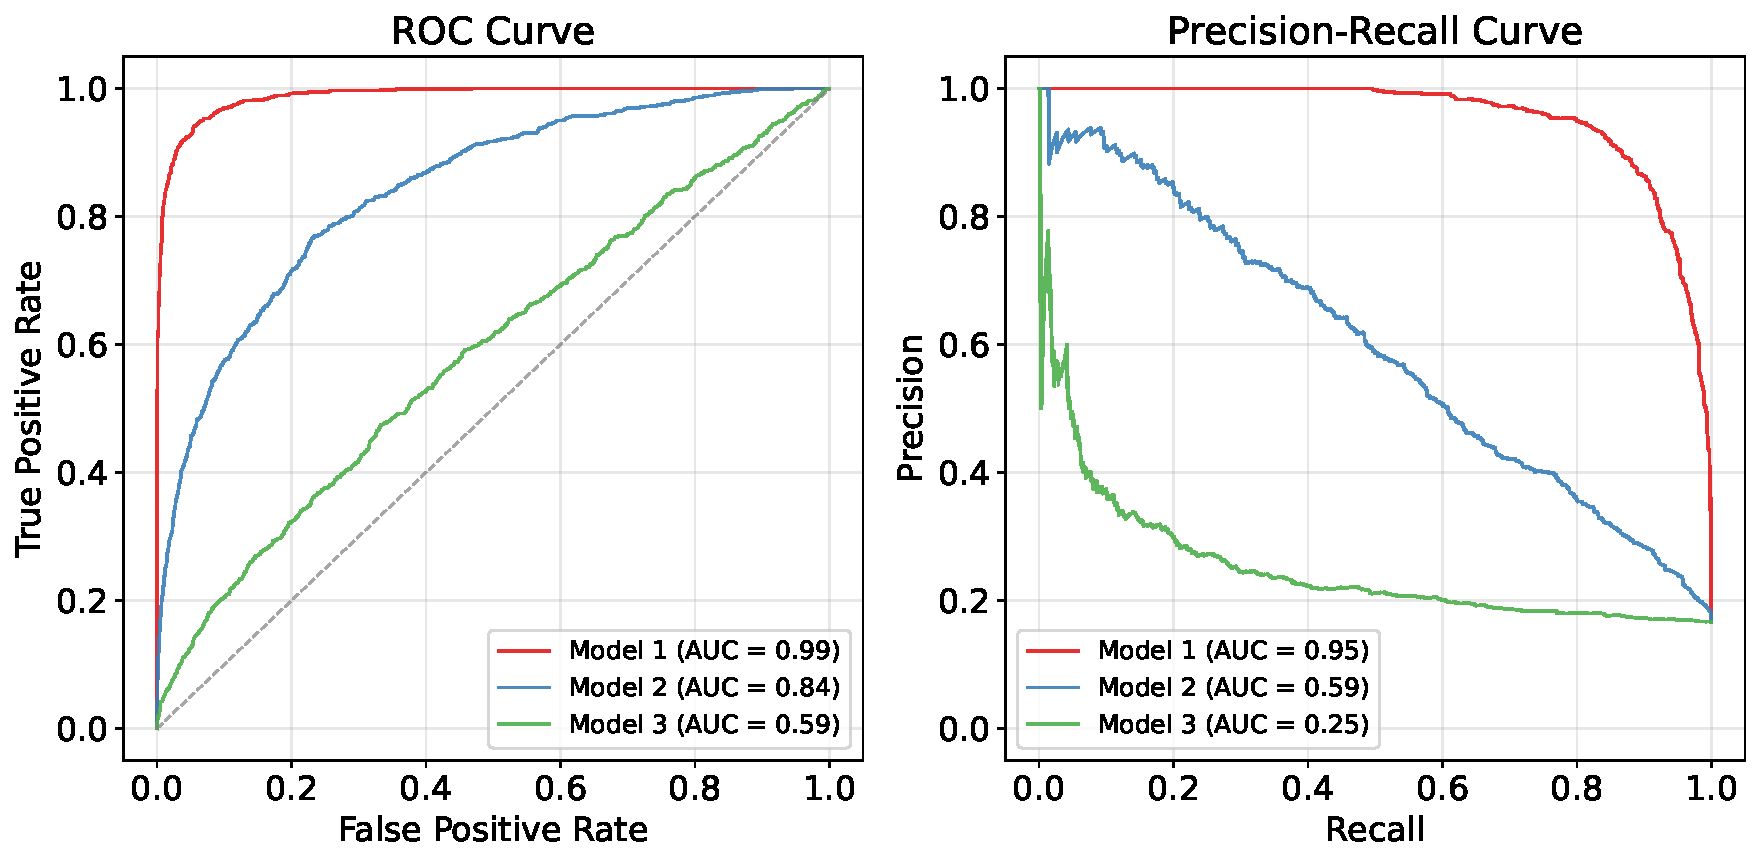
\includegraphics[width=\linewidth]{images/classification_curves.pdf}
        \caption{Examples of three receiver operating characteristic curves and three precision-recall curves.}
        \label{fig:curves}
    \end{figure}

    Figure~\ref{fig:curves} shows what an ROC curve may look like. A diagonal line would mean that the classification is random, and any curve above it shows improved performance. Curves closer to the top left corner signify high TPR and low FPR. Therefore, overall performance is usually summarized by the \textbf{Area Under the Curve (AUC)}. ROC curve can be generalized to multiclass classification by calculating TPR and FPR individually for each class. The resulting curves can be averaged across classes to produce a single line.~\cite{Terven2025, Szeliski2022}

    \item[Precision-Recall (PR) Curve] Similarly to the ROC curve, the PR curve plots precision and recall at various decision thresholds. It is constructed exactly the same way, but contains recall on the x-axis and precision on the y-axis. It displays the precision-recall trade-off, as precision usually drops off with increasing recall. Figure~\ref{fig:curves} shows possible PR curves, which indicate better performance the higher they are. The top right corner corresponds to perfect precision and recall, and therefore the overall performance of the model can also be measured by the AUC. PR curve can be generalized to multiclass classification in the same fashion as the ROC curve by individually calculating the metrics for each class.~\cite{Terven2025}
    
    \item[Top-k Accuracy] Frequently reported metric in large scale multiclass image classification, it defines a prediction as correct if the true class is among the top-k predicted labels with the highest confidence. This metric is often used because the evaluation of multiclass image classification can be ambiguous. For example, an image may contain multiple objects from different classes, making it unclear which object the model should use to determine the final classification of the entire image.~\cite{Terven2025, Russakovsky2015}
\end{description}


\section{Object Detection}
Object detection aims to both locate and identify individual objects within an image by predicting their class and position. Their spatial location and extent are usually expressed as a bounding box, which is an axis-aligned rectangle that tightly bounds the object. Object detection combines classification and localization, making it significantly more demanding than sole classification. It is central to any task that involves analyzing complex scenes containing multiple instances that must be individually recognized. Therefore, object detection forms the basis for solving more complex or high-level tasks, such as scene understanding, object tracking, or event detection.~\cite{Liu2020}

\paragraph{Large scale datasets} Similarly to classification, large labeled datasets have also played a key role in the development of object detection methods. They have established a common ground for measuring and comparing the performance of competing algorithms and have helped advance the field toward more complex and challenging problems~\cite{Liu2020}. Pascal VOC (Visual Object Classes)~\cite{Everingham2010}, with 20 object categories, is a benchmark dataset that standardized object detection evaluation. It contains significant variability in terms of object size, orientation, illumination, and occlusion, with consistent and exhaustive annotations for the specified classes. Despite its influence, Pascal VOC remains relatively small compared to large scale datasets such as ImageNet.

MS COCO (Microsoft Common Objects in Context)~\cite{Lin2014} is a newer dataset that contains complex everyday scenes with common objects in their natural context. It consists of 91 object classes and 2.5 million labeled instances in 328 thousand images. All objects are labeled using instance-level segmentation masks to aid in precise localization. MS COCO focuses on images that reflect the composition of actual everyday scenes. These images usually contain multiple objects from non-iconic views, where the objects are often in the background, partially occluded, or amid clutter, rather than well-centered objects in isolation. This makes object detection more challenging and enables models to perform better in real-world scenarios.

\paragraph{Applications in medicine} In medicine, object detection can help identify and localize specific structures or anomalies, providing spatial information beyond simple classification. It can be used to precisely locate lesions, tumors, or other clinically relevant features within larger images, assisting diagnosis, treatment planning, and monitoring.

For example, distal radius fractures at the wrist are the most common hand fractures and their treatment depends mainly on a diagnosis based on X-ray images. These images are inherently difficult to interpret, so a significant portion is incorrectly diagnosed. Yahalomi et al.~\cite{Yahalomi2019} used transfer learning to train a Faster R-CNN, deep learning object detection neural network, to identify and locate distal radius fractures in anteroposterior X-ray images, as shown in Figure~\ref{fig:fracture}. Their detection model has achieved substantially higher accuracy in detecting fractures than the average radiologist and physician.

\begin{figure}[b]
    \centering
    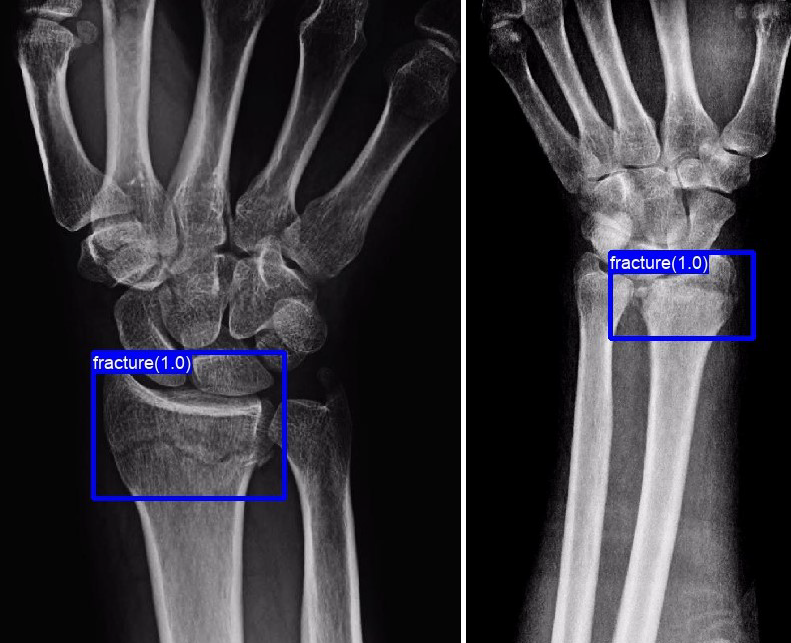
\includegraphics[width=0.4\linewidth]{images/radial_fracture.png}
    \caption{Distal radius fracture detection in augmented X-ray images with enhanced contrast.~\cite{Yahalomi2019}}
    \label{fig:fracture}
\end{figure}

\subsection{Performance Metrics}
Object detection algorithms return a set of bounding boxes for every image, each with the class of the detected object and the confidence of the prediction. These must be evaluated with regard to the set of ground truth bounding box annotations. Object detection metrics must evaluate both the accuracy with which objects are classified and the precision with which they are localized. The localization aspect is taken into account when determining which predictions are correct using \textbf{Intersection over Union (IoU)}:
\begin{equation}\label{eq:iou}
    \text{IoU}(B_1, B_2) = \frac{\text{Area}(B_1 \cap B_2)}{\text{Area}(B_1 \cup B_2)}
\end{equation}
It measures the overlap between two bounding boxes. Examples of its values for different overlaps are shown in Figure~\ref{fig:iou}. A prediction can be correct only if its bounding box overlaps a ground truth box of the same class with the IoU exceeding a set threshold.

\begin{figure}
    \centering
    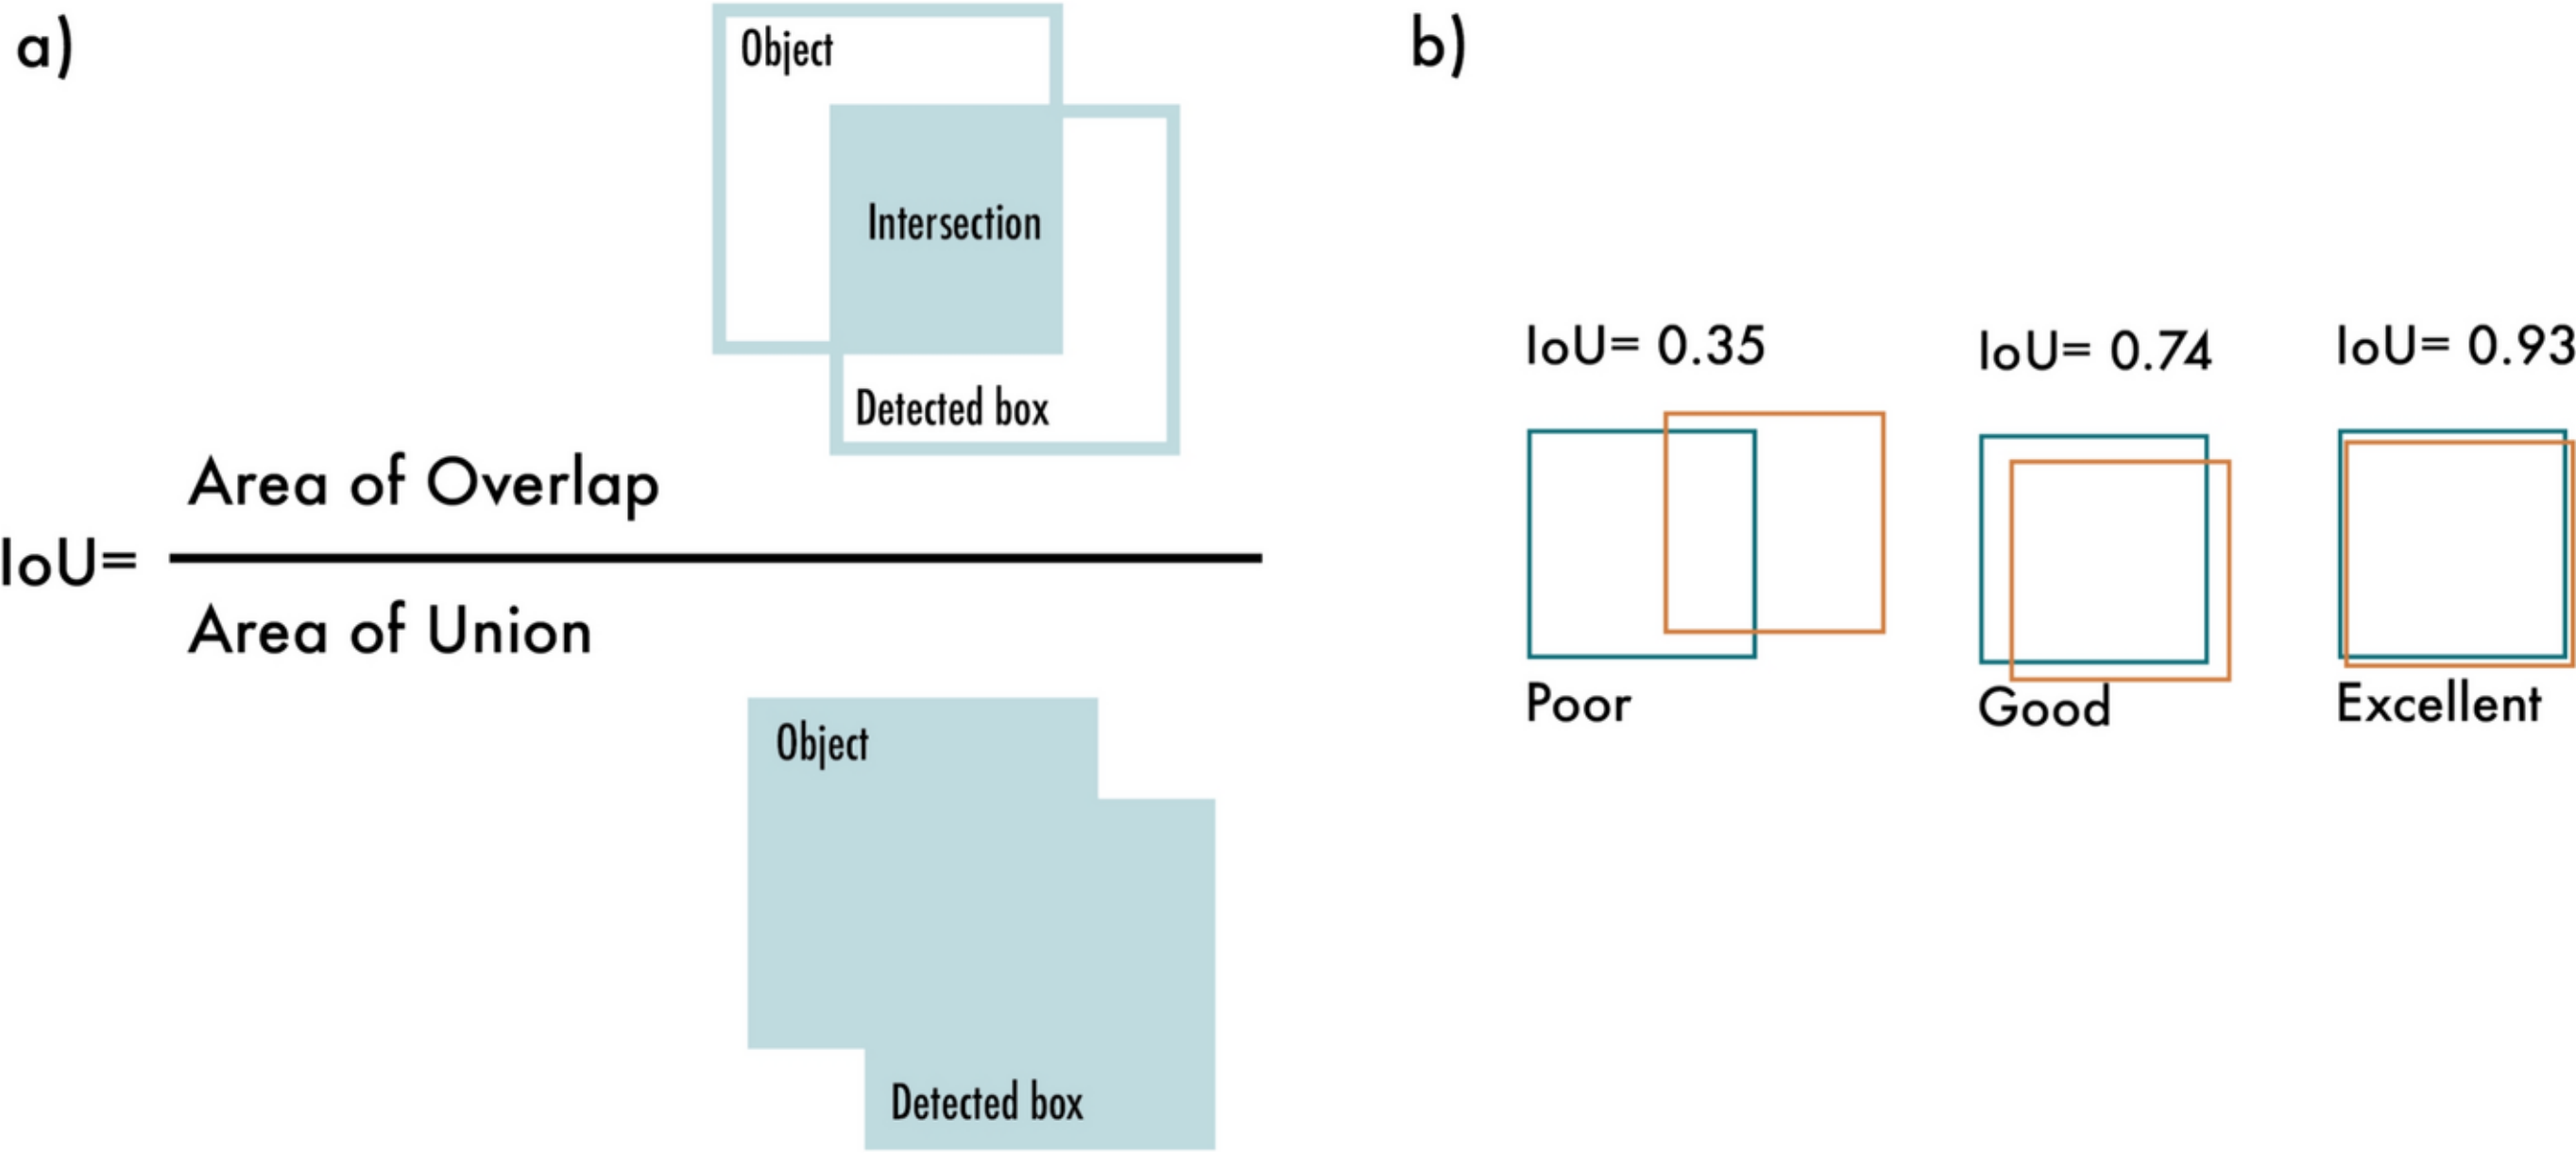
\includegraphics[width=0.8\linewidth]{images/iou.png}
    \caption{a) Intersection over union computed as the ratio of the intersection area of two bounding boxes over the area of their union. b) Examples of three different IoU values for varied box positions.~\cite{Terven2025}}
    \label{fig:iou}
\end{figure}

However, IoU alone is not sufficient to determine which predictions are correct, because there can be a different number of predictions and ground truth annotations. Each ground truth can be matched to at most one prediction and vice versa, but there can be duplicate predictions detecting the same object, or a single prediction that could be interpreted as detecting two different objects. Therefore, predictions need to be matched to ground truth annotations. This is done for each class and image separately according to Algorithm~\ref{alg:matching}. It greedily matches predictions in descending order of confidence to one ground truth label of the same class that has the highest IoU. The resulting matches are then used to construct the confusion matrix, which contains the following fields:
\begin{itemize}
    \item \textbf{True Positive (TP):} number of predictions successfully matched to a ground truth
    \item \textbf{False Positive (FP):} number of predictions not matched to any ground truth, also including duplicate predictions
    \item \textbf{False Negative (FN):} number of ground truth labels not matched to any prediction
    \item \textbf{True Negative (TN):} not defined because there is a very large space of possible bounding boxes that correspond to the background
\end{itemize}

\begin{algorithm}
    \caption{Prediction and ground truth matching algorithm}\label{alg:matching}
    \KwIn{List of predictions $\{(b_i, p_i)\}_{i=1}^N$ of class $C$ for image $I$, where $b_i$ is the bounding box and $p_i$ is prediction confidence \newline
    Set $\mathcal{B}$ of ground truth bounding boxes of class $C$ for image $I$ \newline
    IoU threshold $\tau$}
    \KwOut{Binary list $\{z_i\}_{i=1}^N$ indicating whether prediction $i$ is a true positive detection}
    Sort $\{(b_i, p_i)\}_{i=1}^N$ in descending order of $p_i$\\
    \For{$i = 1, \dotsc, N$}{
        Let $\mathcal{A} = \{b \in \mathcal{B}: \text{IoU}(b_i, b) \geq \tau\}$\\
        \eIf{$\mathcal{A} \neq \emptyset$}{
            Let $b^* = \displaystyle \arg\max_{b \in \mathcal{A}} \text{IoU}(b_i, b)$\\
            $\mathcal{B} = \mathcal{B} \setminus b^*$\\
            $z_i \gets 1$ \tcp{true positive}
        }{
            $z_i \gets 0$ \tcp{false positive}
        }
    }
\end{algorithm}

This process captures the localization aspect of object detection, and the constructed confusion matrix is used to evaluate the classification quality. Performance metrics from image classification can be applied, except those that require the number of true negatives. The metrics that remain applicable are precision, recall, and the F1-score. They are calculated separately for each class, and the overall detection performance is usually summarized using the following metrics.~\cite{Terven2025, Liu2020, Everingham2010}

\begin{description}
    \item[Average Precision (AP)] Precision and recall are typically evaluated together using a PR curve. While the AUC can summarize it in one number, PR curves are often jagged and fluctuate over short intervals, as can be seen in Figure~\ref{fig:curves}. This makes the AUC sensitive to minor changes in prediction ranking. AP is defined as the area under the interpolated PR curve:
    \begin{equation}\label{eq:ap}
        \mathrm{AP} = \frac{1}{|\mathcal{R}|} \sum_{r \in \mathcal{R}} \max_{\tilde{r} \geq r} \text{Precision}(\tilde{r})
    \end{equation}
    where $\text{Precision}(r)$ is the precision at recall $r$, and $\mathcal{R}$ is the set of recall levels used for PR curve interpolation. The interpolation ensures that the curve reflects the highest precision achievable at each recall level, making the area under the curve more robust to small variations in prediction ranking~\cite{Everingham2010}. That is why AP is generally preferred over simple AUC.
    
    The exact PR curve interpolation method can differ depending on the definition. Pascal VOC initially evaluated AP using 11-point interpolation at $\mathcal{R} = \{0, 0.1, 0.2, \dotsc, 1\}$, later switching to interpolation at every point where recall changes~\cite{Everingham2015}. MS COCO applies 101-point interpolation at $\mathcal{R} = \{0, 0.01, 0.02, \dotsc, 1\}$. AP is computed separately for each class, and the overall performance is measured by \textbf{Mean Average Precision (mAP)}, which is the average of AP across all classes. AP depends on the IoU threshold used to match the predictions with ground truth annotations. Common standard AP metrics are defined at different threshold values:
    \begin{itemize}
        \item $\mathbf{AP_{50:95}}$\textbf{:} AP is computed and then averaged over IoU thresholds from the set $\{0.50, 0.55, \dotsc, 0.95\}$, summarizing performance across varying localization strictness
        \item $\mathbf{\mathbf{AP_{50}}}$\textbf{:} AP at $\text{IoU} \geq 0.5$ is used in the Pascal VOC benchmark and balances moderate localization and practical detection requirements
        \item $\mathbf{AP_{75}}$\textbf{:} AP at $\text{IoU} \geq 0.75$ is used in strict scenarios where precise localization is important~\cite{Terven2025, Liu2020, Everingham2010}
    \end{itemize}
\end{description}


\section{Image Segmentation}
Image segmentation divides images into precise regions that correspond to meaningful objects or structures. It can be considered the natural progression from classification and object detection because it provides the most detailed visual understanding, capturing present objects and their exact shape and size. There are two types of image segmentation that differ slightly in their approach and serve distinct purposes: semantic segmentation and instance segmentation. Semantic segmentation performs pixel-level classification, assigning a label from a predefined set of object categories to every pixel. Instance segmentation additionally distinguishes between separate instances of the same class, making it a direct extension of object detection by refining bounding boxes into precise segmented masks.~\cite{Minaee2022}

The creation of datasets for image segmentation is generally more challenging than for other tasks at the image or object level, as it requires a label for every single pixel. The object detection datasets Pascal VOC and MS COCO are also commonly used for segmentation. Pascal VOC provides segmentation annotations for a subset of images, while MS COCO primarily provides instance-level segmentation masks for all of its objects.

\paragraph{Applications in medicine} Segmentation enables analysis of image content at a very fine scale and is essential in tasks where precise boundaries and morphology matter. In medicine, it is important for precise delineation of organs or structures in medical images for accurate diagnosis, treatment, or surgical planning~\cite{Aljuaid2022}.

For example, Havaei et al.~\cite{Havaei2017} used a deep convolutional neural network to segment glioblastomas in MRI images. Glioblastomas are the most aggressive and common type of brain tumors. They can appear anywhere in the brain, in almost any shape or size, and their borders are often fuzzy and hard to distinguish from healthy tissues, making them difficult to segment. The results of their segmentation approach can be seen in Figure~\ref{fig:tumor}. Accurate segmentation of brain tumors can greatly improve diagnostics, growth rate prediction, and treatment planning.

\begin{figure}
    \centering
    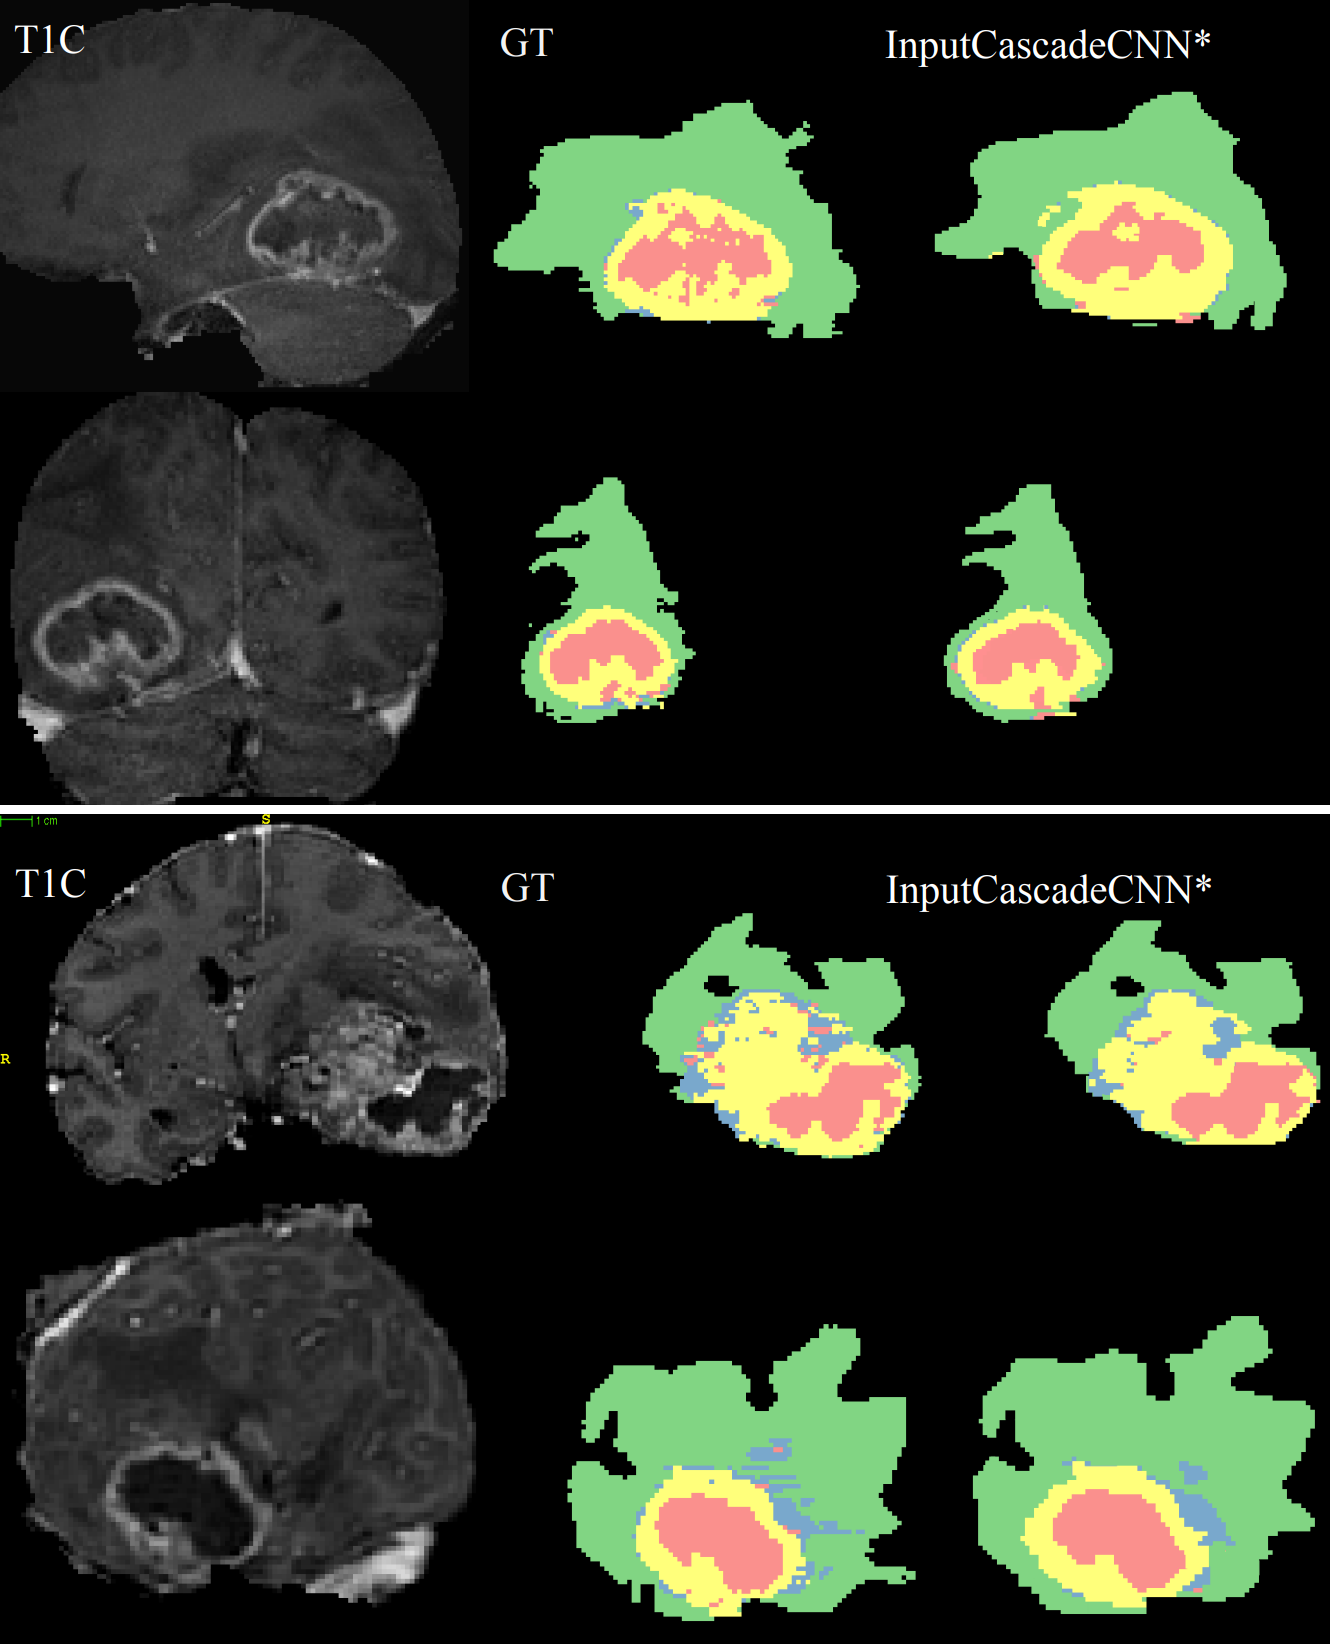
\includegraphics[width=0.5\linewidth]{images/tumor.png}
    \caption{Brain tumor segmentation results showing different tumor regions. The left column displays MRI scans in various views, the middle column shows the corresponding ground truth segmentation masks, and the right column presents the predicted segmentation masks.~\cite{Havaei2017}}
    \label{fig:tumor}
\end{figure}

\subsection{Performance Metrics}
Image segmentation can be treated as pixel-level classification, so a confusion matrix can be easily constructed in the same fashion as described in section~\ref{sec:class}. Standard classification metrics, such as accuracy, precision, recall, or F1-score, can then be applied to each class. In addition, segmentation tasks often employ metrics that better capture the quality of overlap and boundary agreement between the predicted and ground truth masks. These metrics are likewise calculated per class and then averaged to obtain a final score.~\cite{Terven2025, Minaee2022}
\begin{description}
    \item[Intersection over Union (IoU)] Also called the Jaccard Index, it is one of the most popular metrics in semantic segmentation. It measures the degree of overlap between the predicted and ground truth segmentation masks at the pixel level. IoU is defined as the area of intersection divided by the area of union between the two masks. It can also be formulated using the confusion matrix.~\cite{Terven2025, Minaee2022}
    \begin{equation}
        \text{IoU} = \frac{\mathrm{TP}}{\mathrm{TP} + \mathrm{FP} + \mathrm{FN}}
    \end{equation}
    
    \item[Dice Coefficient] Another popular metric for image segmentation, commonly used in medical image analysis tasks. It is also an overlap based metric and is closely related to IoU, with their relationship given by $\text{Dice} = \frac{2\text{IoU}}{1 + \text{IoU}}$. Dice coefficient is defined as two times the overlap area of the predicted and ground truth masks, divided by the sum of their individual areas. It is equivalent to the F1-score and is therefore suitable for images where the foreground and background areas are imbalanced, such as images with very small objects.~\cite{Terven2025, Minaee2022}
    \begin{equation}
        \text{Dice} = \frac{2\mathrm{TP}}{2\mathrm{TP} + \mathrm{FP} + \mathrm{FN}}
    \end{equation}
    
    \item[Boundary F1-Score (BF)] Evaluates segmentation quality by focusing on boundary delineation rather than the overlap of entire masks. BF defines a boundary as a narrow band around every contour. Predicted boundary pixels are compared to ground truth boundaries with a small distance tolerance. BF then determines which pixels overlap and calculates the F1-score. It is suited for tasks where accurate outlines are important, but it may not reflect the segmentation quality of large interior regions. It is complementary to IoU and can be used alongside it.~\cite{Terven2025, Csurka2013}
    
    \item[Masked Average Precision] The standard evaluation metric for instance segmentation, which generalizes the concept of AP to pixel-level segmentation masks. Instead of calculating the IoU of two bounding boxes when determining which predictions are correct, it calculates the IoU of two segmentation masks. Otherwise, masked AP is calculated just like AP in object detection using Equation~\ref{eq:ap}. It evaluates the quality of both the correct object localization and mask segmentation. The IoU threshold can be adjusted to specify the required level of segmentation performance when predictions are evaluated as true or false positives.~\cite{Terven2025}
\end{description}



\chapter{Convolutional Neural Networks}
Over the last decade, Convolutional Neural Network (CNN) models have become the method of choice for most computer vision tasks and today form the backbone of many state-of-the-art computer vision systems. Although initially developed for image classification, these networks have more recently been adapted for a variety of tasks, including object detection, image segmentation, image denoising, or pose estimation.

CNNs were first formalized by LeCun et al.~\cite{Lecun1998} in the form of their LeNet network, which was applied to handwritten digit recognition. However, it was only after the breakthrough publication by Krizhevsky et al.~\cite{Krizhevsky2012} introducing AlexNet that CNNs began to consistently outperform traditional computer vision techniques in natural image classification. AlexNet dramatically reduced the error rate on ImageNet from 25.8\% to 16.4\%. Since then, modern CNN architectures have become deeper, more efficient, and more specialized, with the classification accuracy continuing to improve significantly.~\cite{Szeliski2022}

\paragraph{Traditional computer vision} Before the introduction of CNNs, computer vision systems were generally divided into two modules: a hand-crafted feature extractor and a classifier. The task of the feature extractor was to transform the input into low-dimensional vectors intended to capture meaningful information, while the classifier categorized these feature vectors into classes.

Although classifiers were general purpose and could be built and trained using machine learning algorithms, the performance of the system was largely determined by the feature extractor, which encoded most of the prior knowledge. Designing effective feature extractors required substantial manual effort, relied on domain-specific knowledge, and often failed to generalize to new tasks or datasets.~\cite{Szeliski2022, Lecun1998}

\begin{figure}
    \centering
    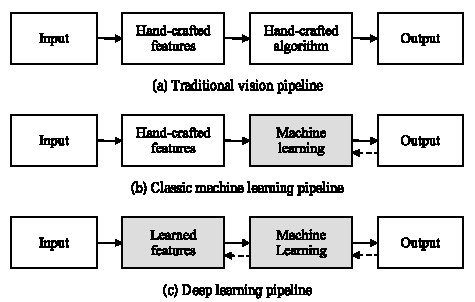
\includegraphics[width=0.8\linewidth]{images/pipelines.pdf}
    \caption{Different computer vision pipelines, where backward arrows indicate learning based on feedback from the following stage. It shows the progression from hand-crafted algorithms to end-to-end training.~\cite{Szeliski2022}}
    \label{fig:pipelines}
\end{figure}

\paragraph{Fully connected neural networks} Deep neural networks can learn complex, high-dimensional, nonlinear mappings from large datasets, which makes them suitable candidates for computer vision tasks. The difference between traditional and deep learning approaches in computer vision is illustrated in Figure~\ref{fig:pipelines}. Deep networks can extract relevant features directly from raw input, effectively combining the functions of feature extractor and classifier in a single model that can be trained end-to-end.

Applying fully connected neural networks directly to flattened image data is possible, but this approach suffers from several limitations. Fully connected networks ignore the spatial structure of the input, so they cannot naturally capture the relationships between neighboring pixels. Additionally, their large number of parameters makes them computationally expensive and prone to overfitting, particularly for high-resolution images.~\cite{Lecun1998}

\paragraph{Essential CNN principles} Convolutional neural networks overcome these limitations by incorporating the inherent properties of images directly into their architecture. They explicitly preserve spatial relationships between pixels by maintaining the two-dimensional structure of the input throughout the network and utilize sparse connectivity and weight sharing.

Through sparse connectivity, each neuron in a convolutional layer is connected only to a local neighborhood of the input, reducing the total number of connections and focusing on the extraction and combination of local features. Weight sharing replicates the weight configurations across the entire input, allowing the network to detect features regardless of their location and providing shift invariance with respect to translations or local distortions.

These principles greatly reduce the number of trainable parameters, which facilitates end-to-end training. By learning all parameters directly from the raw input, CNNs eliminate the need for manual feature engineering and can adapt flexibly to a wide range of visual tasks.~\cite{Lecun1998}


\section{Architecture}
Convolutional neural networks are composed of a sequence of layers stacked to progressively extract and process features from an input image. The core component of the architecture is the trainable convolutional layer, which is primarily responsible for feature extraction. CNN layers consist of multiple feature maps, or channels, each made up of neurons arranged in a two-dimensional grid. Each neuron receives input only from a small spatial region in the previous layer, determined by the local connectivity of the convolution. This region is referred to as the receptive field of the neuron. The principle of connecting neurons to a local receptive field is analogous to the locally sensitive, orientation-selective neurons identified in the visual cortex of animals by Hubel and Wiesel~\cite{Hubel1962}. This design allows the network to detect spatially localized patterns and features.

\begin{figure}[b]
    \centering
    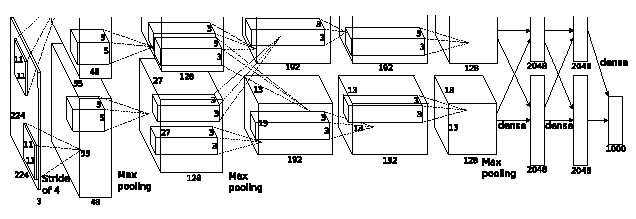
\includegraphics[width=\linewidth]{images/alexnet.pdf}
    \caption{AlexNet architecture showing five convolutional layers followed by three fully connected (dense) layers. The channels of the layers are split between two GPUs and are interconnected only at certain layers.~\cite{Krizhevsky2012}}
    \label{fig:alexnet}
\end{figure}

The overall architecture consists of multiple convolutional layers, typically followed by an activation function, which are alternated with pooling layers that reduce the spatial resolution of the feature maps. An example is shown in Figure~\ref{fig:alexnet}, which presents the AlexNet architecture. The number of channels typically increases in deeper layers while their spatial dimensions decrease. This progressive reduction in spatial resolution, compensated for by richer feature representations, allows the network to achieve a degree of invariance to geometric transformations of the input images.

The stacked convolutional and pooling layers form a feature extractor that transforms the raw input into a higher-level representation. These features are usually passed to one or more fully connected layers that aggregate the extracted information to produce a task-specific output, such as a classification label or a probability distribution over multiple classes.~\cite{Szeliski2022, Lecun1998, Zhao2024, Krichen2023}

\paragraph{Feature hierarchy}
The main task of a CNN is to construct local features and progressively transform them into more discriminative and semantically meaningful representations suitable for decision-making. This hierarchical feature representation emerges from the stacked structure of the network. Early layers detect local visual patterns, such as oriented edges, corners, or endpoints, since their receptive fields cover only a small part of the input. Subsequent layers combine these patterns to detect more complex and higher-level features.

As the receptive fields of neurons expand in deeper layers, the network gradually integrates information over larger portions of the input. After several convolutional layers, the receptive field can span the entire image, capturing global context. The deepest layers then integrate all detected patterns into high-level semantic features, representing meaningful structures or objects in the input image. This hierarchical organization allows CNNs to extract increasingly abstract information at each successive layer while maintaining spatial relationships from the original input.~\cite{Szeliski2022, Lecun1998, Krichen2023}

\subsection{Convolutional Layer}
A convolutional layer consists of a set of feature maps, each obtained by applying convolution and linear combination to the feature maps in the previous layer. Convolution is a linear filtering operation in which each output pixel is computed as a weighted sum of pixels within a local neighborhood, determined by the weights of the convolution kernel or filter. In classical image processing, filters can be designed to add blur, sharpen details, accentuate edges, or remove noise. The convolution operator is defined as:
\begin{equation}
    (f \ast h)(i, j) = \sum_k \sum_l f(i - k, j - l)h(k, l)
\end{equation}
where $f$ is the input image, $h$ is the convolution filter, and $k$ and $l$ are its signed offsets. The filter is applied repeatedly across the input image, producing the transformed output, as shown in Figure~\ref{fig:convolution}.

\begin{figure}
    \centering
    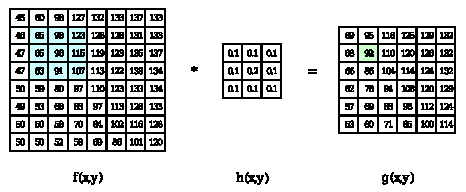
\includegraphics[width=\linewidth]{images/convolution.pdf}
    \caption{Example of convolution, where the input image on the left is convolved with the kernel in the middle to produce the output on the right. The blue pixels indicate the neighborhood used to compute the green pixel in the output.~\cite{Szeliski2022}}
    \label{fig:convolution}
\end{figure}

A common alternative to convolution is the correlation operator, which differs only in the orientation of the kernel during computation. Convolution flips the kernel both horizontally and vertically, while correlation applies it directly. These operators are often not distinguished because filters in image processing are usually symmetric and flipping them has no effect, and in CNNs the filters are learned during training, where the correct orientation is automatically acquired. The correlation operator is defined as:
\begin{equation}
    (f \star h)(i, j) = \sum_k \sum_l f(i + k, j + l)h(k, l)
\end{equation}
The following equation shows the equivalence between correlation and convolution with a flipped kernel. Flipping the kernel is achieved by reversing its offsets during the calculation, and since the summation is over all signed offsets, the same terms are included, just in reverse order:
\begin{equation}
    \sum_k \sum_l f(i + k, j + l)h(k, l) = \sum_k \sum_l f(i - k, j - l)h(-k, -l)
\end{equation}

Unlike classical image processing, where a filter is applied independently to each input channel, convolutions in CNNs linearly combine all $C_{in}$ input channels. Each output channel is computed by applying a separate kernel to each input feature map and summing the results with a bias term. This process is illustrated in Figure~\ref{fig:conv_layer} and allows the network to construct local features and combine them to form more discriminative representations. Each output feature map is created by the following operation:
\begin{equation}
    y(c_2) = \sum_{c_1 = 1}^{C_{in}} x(c_1) \star w(c_1, c_2) + b(c_2)
\end{equation}
where $y(c_2)$ is the output feature map, $x(c_1)$ are the input feature maps, $w(c_1, c_2)$ is the convolution filter for the corresponding channel combination, and $b(c_2)$ is the additive bias. Although the layer is conventionally called a convolutional layer, in practice the correlation operator is used instead to avoid unnecessary kernel flipping. The distinction is generally glossed over because training automatically adapts the filter orientation.~\cite{Szeliski2022, Krichen2023}

\begin{figure}
    \centering
    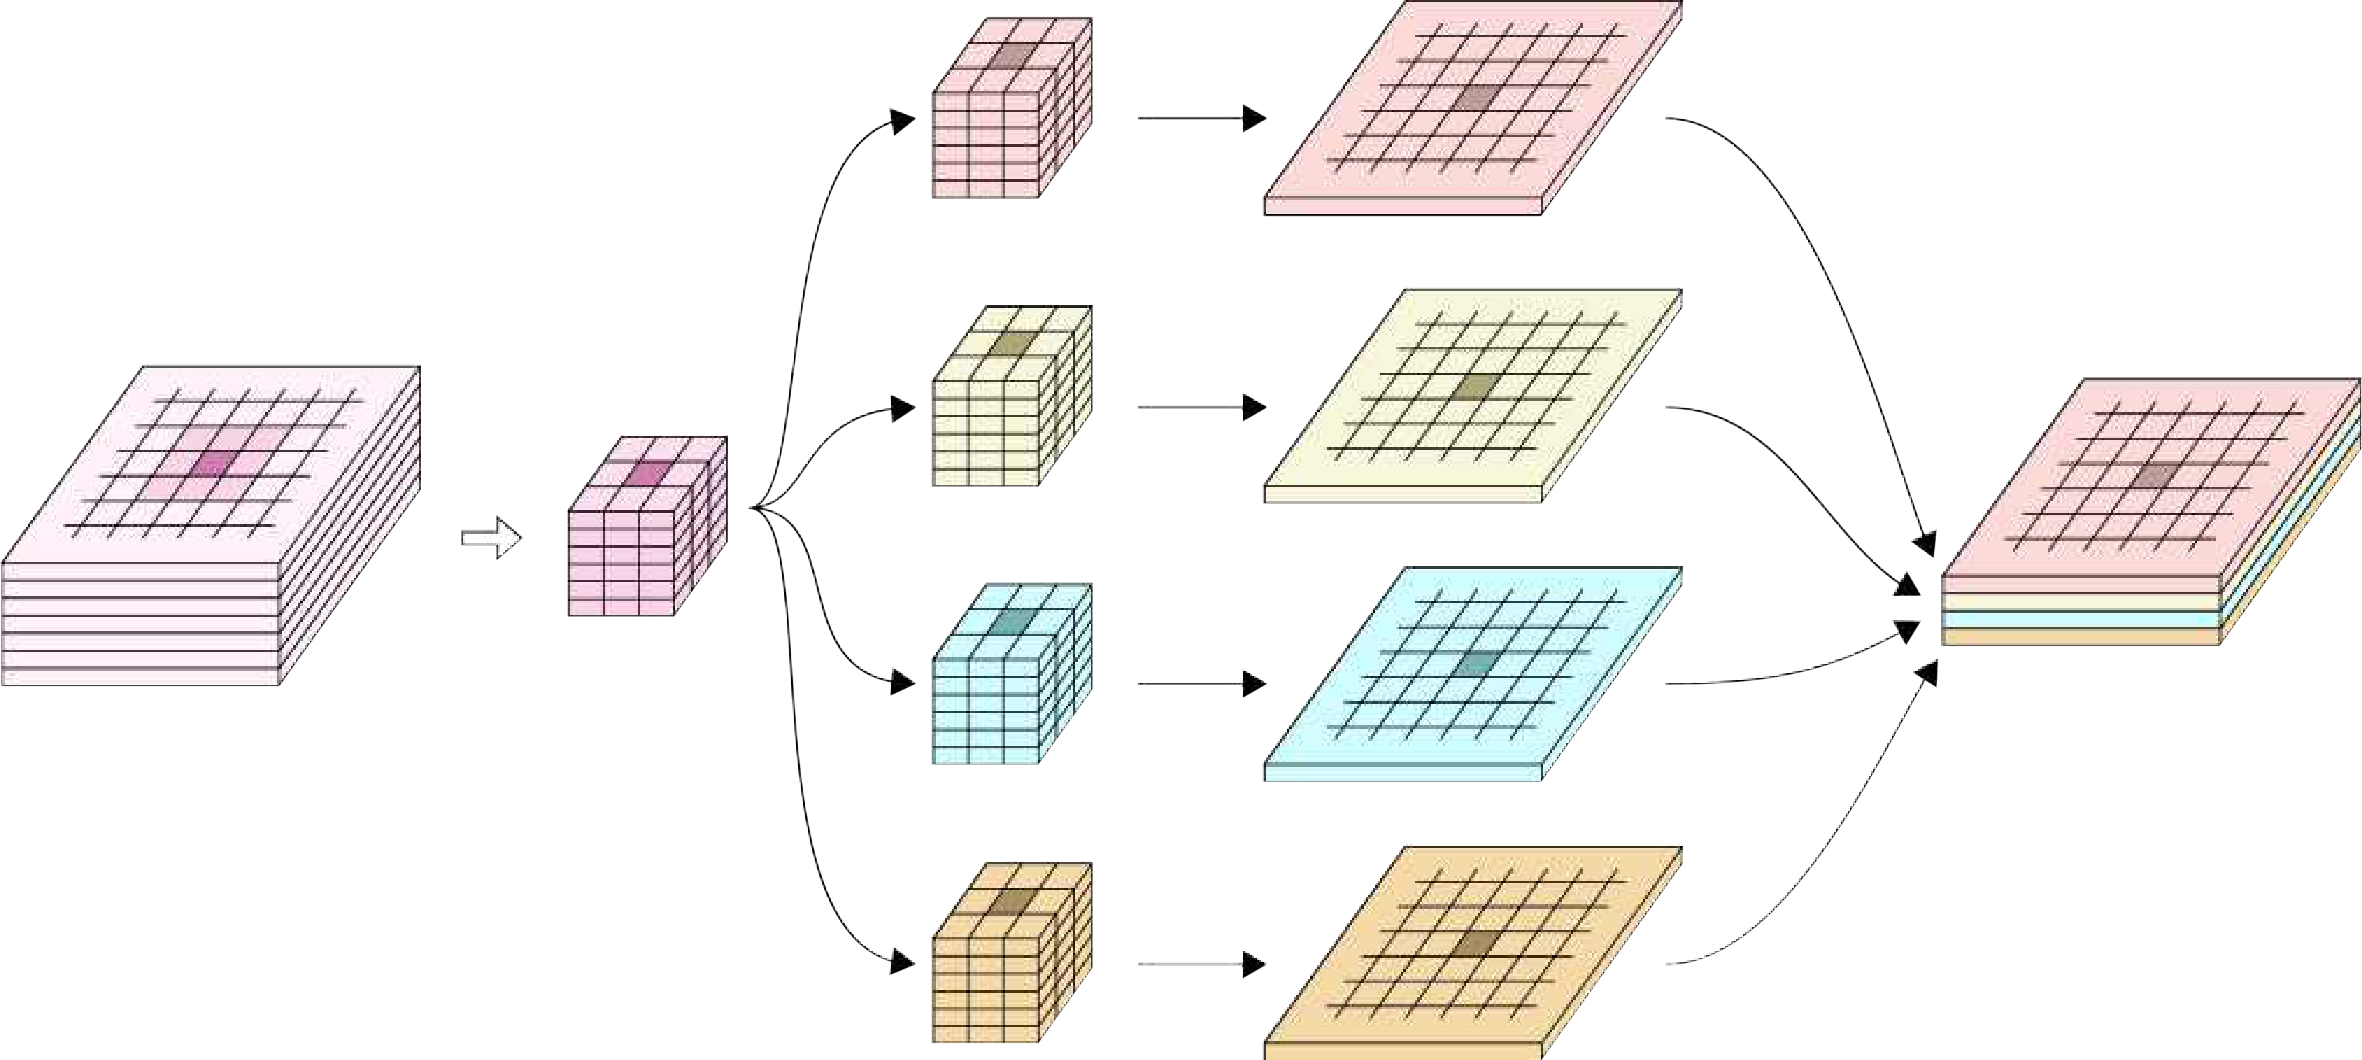
\includegraphics[width=0.9\linewidth]{images/conv_layer.png}
    \caption{Convolutional layer with six input channels and four output channels. Each input feature map on the left is convolved with a separate kernel for each output channel to produce resulting feature maps on the right. Every output channel has six convolution filters of size $3 \times 3$ each with different parameters.~\cite{Szeliski2022}}
    \label{fig:conv_layer}
\end{figure}

The behavior of convolutional layers also depends on several hyperparameters that determine how exactly the convolution kernel is shifted over the input feature map during computation. These hyperparameters include:
\begin{itemize}
    \item \textbf{Padding:} Applying convolution reduces the spatial dimensions of the feature map because the neighborhoods of the operation extend beyond the input near its edges. The amount of shrinkage depends on the kernel size. To preserve the spatial resolution, the input feature maps can be padded using methods such as zero padding, constant padding, or edge replication.

    \item \textbf{Stride:} The typical stride is 1, which means that the kernel shifts by one pixel between consecutive convolution evaluations. Using a larger stride computes the convolution at every $n$-th position horizontally and vertically. This significantly shrinks the output and can be used to reduce the resolution of the feature map.
    
    \item \textbf{Dilation:} Dilated convolution inserts empty rows and columns between kernel elements. This increases the effective receptive field in the previous layer without increasing the number of parameters.

    \item \textbf{Grouping:} Convolutional layers usually use all input channels to produce each output channel. However, the input and output channels can be partitioned into groups, with convolutions applied only within each group. AlexNet, shown in Figure~\ref{fig:alexnet}, uses grouped convolution to distribute computation between two GPUs.
\end{itemize}

All learnable parameters of a convolutional layer are contained in its convolution kernels, with the exception of biases. Every output channel has one bias and $C_{in}$ kernels. If the kernel has spatial dimensions $K_w \times K_h$, each channel in the layer contains $1 + K_wK_hC_{in}$ parameters. Therefore, a convolutional layer with $C_{out}$ channels contains in total $C_{out} + K_wK_hC_{in}C_{out}$ learnable parameters. This structure is illustrated in Figure~\ref{fig:conv_layer}, which shows the dimensions of all the kernels used.~\cite{Szeliski2022, Krichen2023}

\paragraph{Sparse connectivity and weight sharing}
In this section, a convolutional layer has been defined as a set of feature maps produced by the convolution of feature maps from the previous layer. For better comparison with fully connected neural networks, the individual units in these maps can be viewed as neurons. Their connections are determined by the convolution pattern, and the convolution kernel represents the set of connecting weights used by every neuron in a single feature map. This design enforces sparse connectivity and weight replication within the CNN, which significantly reduce the number of learnable parameters and provide some degree of shift and distortion invariance.

In fully connected networks, every neuron receives input from every unit in the previous layer. In a convolutional layer, neurons are connected only to a small local neighborhood. This considerably reduces the number of connections throughout the network and enables the detection of local features or patterns, since configurations of neighboring pixels often fall into a limited number of categories such as edges or corners. Additionally, elementary feature detectors useful in one region of an image are likely to be useful across the entire image. This is implemented by constraining neurons within the same feature map to share the same set of weights. All neurons in a feature map therefore apply the same convolution kernel, allowing the same feature to be detected at all spatial locations of the input. This further reduces the number of parameters relative to fully connected networks.

Different feature maps within the same layer use different kernels to extract distinct types of local features. Each layer therefore contains multiple feature maps to extract multiple features at each location. If the input is shifted, the output of the convolution shifts by the same amount, but its values remain unchanged otherwise. This property is the basis for the robustness of CNNs to shifts and distortions of the input.~\cite{Lecun1998}

\subsection{Pooling Layer}
Once a feature has been detected, its exact location becomes less important, and only its approximate position relative to other features is relevant. Encoding the precise position can even be detrimental because the location of the same feature often varies between different instances of a class. A simple way to reduce the spatial precision of feature maps is to reduce their resolution. This is achieved using a pooling layer, which performs local subsampling and thereby reduces both the spatial resolution of the feature map and the sensitivity of the network to small shifts and distortions.~\cite{Lecun1998}

A pooling layer connects each of its units to a local receptive field within the corresponding feature map of the previous layer. It operates on each feature map independently and can be viewed as a grid of pooling units spaced $n$ pixels apart, each summarizing an $m \times m$ neighborhood centered at its location. Conceptually, it functions similarly to a convolution with stride $n$ and kernel size $m \times m$, but unlike convolutional layers, pooling layers contain no learnable parameters.

The most commonly used pooling operations are average pooling and max pooling. \textbf{Average pooling} computes the mean value of all elements in its receptive field and is equivalent to a strided convolution with a kernel that contains identical weights summing to one. \textbf{Max pooling} selects the maximum value within its receptive field, extracting the strongest local response. Pooling windows overlap when the stride is smaller than the window size. Overlapping pooling has been observed to slightly reduce overfitting. Overall, pooling layers effectively reduce data dimensionality and encourage invariance to small local shifts.~\cite{Szeliski2022, Krizhevsky2012, Zhao2024}

\subsection{Activation Functions}
Neural networks use activation functions to introduce point-wise nonlinearity, applied to all neurons in hidden layers. This nonlinearity allows the network to learn more complex features and approximate arbitrary nonlinear functions~\cite{Zhao2024, Krichen2023}. The most commonly used activation functions in early neural networks were the \textbf{logistic sigmoid} and the \textbf{hyperbolic tangent (tanh)}:
\begin{equation}\label{eq:sigmoid}
    \sigma(x) = \frac{1}{1 + e^{-x}}
\end{equation}
\begin{equation}
    \tanh(x) = \frac{e^x - e^{-x}}{e^x + e^{-x}}
\end{equation}
The hyperbolic tangent is also a sigmoidal function and is generally preferred over the logistic sigmoid due to its wider output range and more gradual gradient, which often leads to more robust optimization. However, deep neural networks with sigmoidal activations can suffer from the vanishing gradient problem, which slows optimization convergence and can potentially cause the network to settle in a poor local minimum.

The rectified linear function provides an alternative to sigmoidal nonlinearities by addressing these issues. A neuron using this activation is called a \textbf{Rectified Linear Unit (ReLU)}, defined as:
\begin{equation}
    \operatorname{ReLU}(x) = \max(x, 0) = \begin{cases} x, & x > 0\\ 0, & \text{otherwise} \end{cases}
\end{equation}
ReLU is active when the neuron's weighted sum is greater than zero. Computation along the paths of active units is linear, allowing gradients to flow efficiently. Consequently, vanishing gradients are avoided along these active paths, even in arbitrarily deep networks.

ReLU is also computationally efficient because it does not require evaluating exponential functions. Additionally, it produces sparse representations by outputting zero when inactive, which provides mathematical advantages and can be helpful when using hidden layer outputs as features for a classification problem. Deep CNNs with ReLUs train significantly faster than equivalent networks with hyperbolic tangent units, greatly improving performance on large models and datasets~\cite{Krizhevsky2012}.

However, the hard saturation of ReLU at zero can block gradient backpropagation, particularly if an entire layer has no active neurons. This can slow training in a manner similar to the vanishing gradient problem. To mitigate this, variants such as \textbf{Leaky ReLU (LReLU)}~\cite{Maas2013} or \textbf{Parametric ReLU (PReLU)}~\cite{He2015} have been proposed:
\begin{equation}
    \operatorname{LReLU}(x) = \max(x, 0.01x) = \begin{cases} x, & x > 0\\ 0.01x, & \text{otherwise} \end{cases}
\end{equation}
\begin{equation}
    \operatorname{PReLU}(x) = \max(x, 0) + a\min(0, x) = \begin{cases} x, & x > 0\\ ax, & \text{otherwise} \end{cases}
\end{equation}
LReLU allows a small non-zero gradient when the unit is inactive, sacrificing strict zero sparsity for a more robust optimization. PReLU generalizes LReLU by introducing a learnable parameter $a$, which can be either shared across all units in a single channel or across an entire layer.~\cite{Maas2013, Glorot2011}

\subsection{Output Layers}
After feature extraction performed by convolutional and pooling layers, the resulting features must be transformed into a task-specific output. One approach is to flatten the feature maps into a vector and pass them through one or more fully connected layers, followed by a final output layer with an appropriate activation function. Each neuron in a fully connected layer computes a weighted sum of all inputs from the previous layer with an added bias term. The output of a fully connected layer is a vector defined as:
\begin{equation}
    \mathbf{y} = \mathbf{W} \mathbf{x} + \mathbf{b}
\end{equation}
where $\mathbf{x}$ is the input vector, $\mathbf{W}$ is the weight matrix of the layer, and $\mathbf{b}$ are the biases.~\cite{Szeliski2022, Zhao2024}

Alternatively, the feature maps can be aggregated using \textbf{global pooling}, which produces a vector containing one value per channel in the last convolutional or pooling layer. This vector can then be processed by several fully connected layers or, preferably, passed directly to the final output layer with only the activation function applied. Aggregating spatial features using global pooling reduces the number of parameters, helps prevent overfitting, and preserves channel-wise information.~\cite{Lin2014_nin}

\begin{figure}
    \centering
    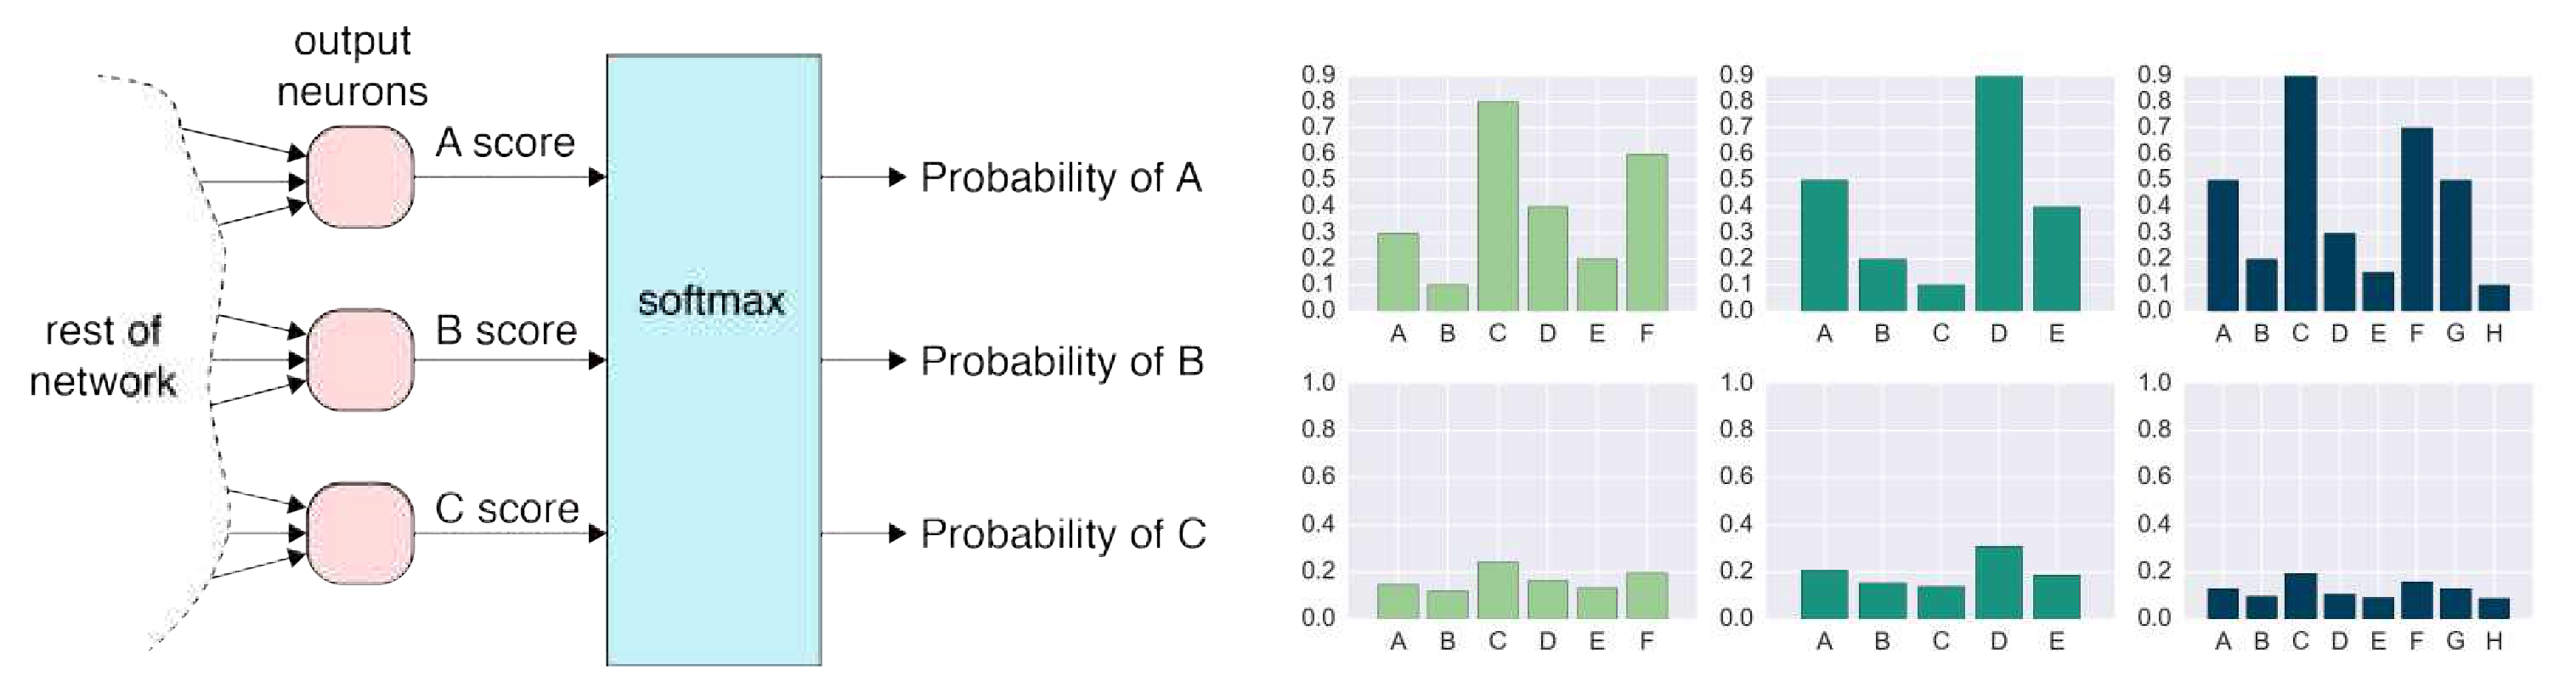
\includegraphics[width=\linewidth]{images/softmax.png}
    \caption{A softmax layer used to convert neural network outputs (logits) into class probabilities. The top row of the graphs shows the logits, while the bottom row shows the softmax normalized probabilities.~\cite{Szeliski2022}}
    \label{fig:softmax}
\end{figure}

The final layer of a CNN produces the task-specific output, which is determined by the number of neurons and the chosen activation function. For regression, the final layer typically consists of one or more neurons with a linear activation function that produces continuous values. When performing classification, the output is usually normalized to represent class probabilities. A single neuron with a sigmoid activation function, defined in Equation~\ref{eq:sigmoid}, can produce the probability for binary classification.

For multi-class classification, the outputs of the final layer, commonly called logits, are converted into class probabilities using the \textbf{softmax} activation function, as illustrated in Figure~\ref{fig:softmax}. Softmax normalizes the output so that the resulting probabilities sum to one. The function is defined as:
\begin{equation}
    \operatorname{softmax}(\mathbf{x})_k = \frac{\exp (x_k)}{\sum_{j=1}^C \exp (x_j)}
\end{equation}
where $C$ is the number of classes and $\mathbf{x}$ is the vector of logits from the final layer. The value $\operatorname{softmax}(\mathbf{x})_k$ represents the probability that the network input belongs to class $k$.~\cite{Szeliski2022, Zhao2024}

\subsection{Training and Loss Functions}
Training a CNN follows the same procedure as training a standard neural network, using backpropagation to compute gradients of a loss function with respect to each trainable parameter and applying an optimization algorithm to update the weights. A differentiable loss function must be defined to quantify how well the network predictions match the target values. The learning problem then consists of finding the parameters that minimize the average loss over a training set $\{(x_1, y_1), \dotsc, (x_N, y_N)\}$, which serves as an estimate of the underlying data distribution. The average loss function is defined as:
\begin{equation}
    E(\mathbf{w}) = \frac{1}{N} \sum_{i = 1}^N L(y_i, f(x_i; \mathbf{w}))
\end{equation}
where the loss $L$ measures the discrepancy between the ground truth $y_i$ and the predicted output $f(x_i; \mathbf{w})$ for the input sample $x_i$ and the collection of adjustable model parameters $\mathbf{w}$.~\cite{Szeliski2022, Lecun1998}

Networks that perform regression of one or more variables commonly use the $L_2$ loss, which penalizes larger errors more severely, or the more robust $L_1$ loss, which is less sensitive to outliers. Classification neural networks use the cross-entropy loss function because their output is usually normalized to represent class probabilities. Binary cross-entropy loss maximizes the likelihood of correct predictions by minimizing their negative log likelihood:
\begin{equation}
    L_{BCE}(y, \hat{y}) = -(y\log\hat{y} + (1 - y)\log(1 - \hat{y}))
\end{equation}
where $y \in \{0, 1\}$ is the ground truth class label of the training sample $x$ and $\hat{y}$ is the predicted probability.

It can be generalized to categorical cross-entropy loss, which sums the negative log likelihoods of the correct class for each training sample:
\begin{equation}\label{eq:cce}
    L_{CCE}(y, \hat{y}) = -\log\hat{y}_y
\end{equation}
where $\hat{y}_k$ is the predicted probability of class $k$ for sample $x$, and $y$ is the ground truth class. Although the outputs of classification networks are commonly interpreted as probability distributions, they do not necessarily represent calibrated probabilities. The training loss encourages high confidence in the correct predictions, but does not ensure that predicted confidence values reflect true likelihoods.~\cite{Szeliski2022}

\begin{figure}[b]
    \centering
    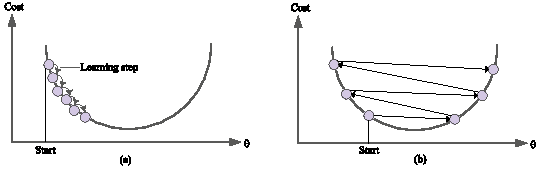
\includegraphics[width=\linewidth]{images/learning_rate.pdf}
    \caption{Gradient descent with suboptimal learning rates. a) Learning rate is too low, resulting in slow convergence. b) Learning rate is too high, resulting in overshooting the minimum or even divergence.~\cite{Zhao2024}}
    \label{fig:learning_rate}
\end{figure}

\paragraph{Gradient descent} The general problem of minimizing a function with respect to a set of parameters can be addressed using gradient-based learning. Neural networks are trained using gradient descent or one of its variants, which iteratively update the parameters until they converge to values that provide an acceptable level of performance on the training and validation datasets. The gradient of the loss function $E$ with respect to the weights $\mathbf{w}$ is calculated using \textbf{backpropagation}~\cite{Rumelhart1986}, which propagates errors backward through the network by evaluating derivatives on the reversed computational graph.

Deep learning models and datasets are too large for computing gradients over the entire training set. Instead, \textbf{Stochastic Gradient Descent (SGD)} approximates the gradient using individual samples. Because this approximation is too noisy in practice, the loss and gradient are typically computed over small subsets of data, called minibatches. The network parameters are then updated by taking a step in the direction opposite to the minibatch gradient. The size of the step is determined by the \textbf{learning rate}, which must be chosen carefully to ensure steady progress without overshooting the optimum. The impact of an incorrectly chosen learning rate is illustrated in Figure~\ref{fig:learning_rate}. It is common to start with a higher value that is gradually decreased during training to improve convergence.

Although standard SGD is effective, it can stall in flat regions of the loss gradient. Several more advanced optimization algorithms have been developed that extend SGD. The most widely used optimizers for deep neural networks are \textbf{Adam}~\cite{Kingma2014} and its decoupled weight decay variant \textbf{AdamW}~\cite{Loshchilov2019}, which combine elements of many previous ideas, such as momentum and adaptive learning rates, into a single framework. Despite these improvements, selecting an appropriate learning rate is important and applying a decreasing schedule can still be beneficial.~\cite{Szeliski2022, Lecun1998, Krichen2023}

\subsection{Normalization Layer}
When the distribution of input data to a neural network changes, the model experiences a covariate shift that can reduce its generalization performance. The same principle applies internally, where the inputs to each layer depend on the parameters of all preceding layers, and small parameter updates accumulate as the network becomes deeper. As training progresses, the input distribution of each layer therefore changes, forcing the layer to continuously adapt. This complicates the optimization of deep neural networks, slows down training by requiring lower learning rates and careful parameter initialization, and makes deep models with sigmoidal nonlinearities particularly difficult to train.

The change in the distribution of layer inputs caused by updates to network parameters is known as the internal covariate shift. \textbf{Batch normalization}~\cite{Ioffe2015} addresses this issue by normalizing neuron outputs throughout the network, which prevents small changes in layer parameters from being amplified as data propagates through a deep network. It fixes the distribution of neuron outputs by transforming them to have zero mean and unit variance. This normalization step is integrated directly into the network architecture so that it is handled appropriately during training.

For a minibatch $\mathcal{B}$ of size $m$, the output of every neuron is normalized independently before being passed to the activation function. The mean $\mu_\mathcal{B}$ and variance $\sigma_\mathcal{B}^2$ are estimated for each neuron across the minibatch samples to calculate the normalized output $\hat{x}_i$:
\begin{equation}
     \mu_\mathcal{B} = \frac{1}{m} \sum_{i = 1}^m x_i
\end{equation}
\begin{equation}
    \sigma_\mathcal{B}^2 = \frac{1}{m} \sum_{i = 1}^m (x_i - \mu_\mathcal{B})^2
\end{equation}
\begin{equation}
    \hat{x}_i = \frac{x_i - \mu_\mathcal{B}}{\sqrt{\sigma_\mathcal{B}^2 + \epsilon}}
\end{equation}
where $x_i$ is the pre-activation value of the neuron $x$ for the training sample $i$ and $\epsilon$ is a small constant for numerical stability.

Because normalization alone can limit what a layer is able to represent, two learnable parameters $\gamma$ and $\beta$ are introduced for each neuron to shift and scale the normalized values $\hat{x}_i$:
\begin{equation}
    y_i = \gamma\hat{x}_i + \beta \equiv \operatorname{BN}_{\gamma, \beta}(x_i)
\end{equation}
These parameters are trained jointly with the rest of the network and allow batch normalization to preserve the representational capacity of the model. The original neuron bias becomes unnecessary because its effect is canceled by mean subtraction and is replaced by the shift parameter $\beta$.

A batch normalization layer, defined by the transformation $\operatorname{BN}_{\gamma, \beta}(x)$, is typically placed directly before the nonlinear activation functions in the neural network architecture. Models with batch normalization can be trained using SGD or any of its variants, which update both the original model parameters and the new normalization parameters. During inference, the mean and variance used for normalization are fixed and estimated over the entire training dataset. In convolutional layers, normalization follows the weight sharing principle by using identical parameters for calculations in different parts of the same feature maps. All neurons within the same feature map are normalized using the same statistics and therefore share one pair of parameters $\gamma$ and $\beta$ per channel.

Batch normalization substantially accelerates the training of deep neural networks by stabilizing the input distributions of their layers. It reduces the sensitivity of gradients to the scale of the network parameters and their initial values. This enables the use of much higher learning rates without the risk of divergence. It also provides a regularizing effect, which reduces the need for dropout, and mitigates vanishing gradients sufficiently to allow the use of sigmoidal nonlinearities.~\cite{Ioffe2015}

Since the introduction of batch normalization, many normalization variants have been proposed. They differ primarily in how they compute the mean and variance used for normalization. Layer normalization~\cite{Ba2016} computes these statistics over all neurons in a layer for each training sample individually, allowing identical computation during training and inference. Instance normalization~\cite{Ulyanov2017} also operates on individual training samples but normalizes each channel independently. Group normalization~\cite{Wu2018} normalizes predefined groups of channels together within each training sample. These methods allow normalization in settings where batch statistics are inaccurate, such as models that require very small batches constrained by memory consumption.~\cite{Szeliski2022}


\section{Regularization}
Deep neural networks contain a large number of parameters, which makes them highly expressive but also prone to overfitting. Overfitting occurs when a model performs well on training data but fails to generalize to new unseen data. While training algorithms aim to minimize the loss on the training dataset, the actual objective is to achieve good generalization, typically estimated using validation error measured on a separate dataset. Regularization methods help prevent neural networks from overfitting by reducing the effective capacity of the model, either by reducing the number of dimensions of the parameter space or by limiting the effective size of each dimension.~\cite{Krichen2023, Prechelt1998}

\paragraph{Early stopping} During training, the generalization error on unseen data often begins to increase at some point, while the training loss continues to decrease. Validation error can be monitored to detect when overfitting begins, and training can be stopped early to prevent it. Early stopping is widely used due to its simplicity and effective regularization performance. Selecting an exact stopping criterion usually involves balancing training time with generalization performance.~\cite{Prechelt1998}

\paragraph{P-norm regularization} Another way to reduce the overfitting of neural networks is p-norm regularization, which modifies the loss function by adding a penalty term that discourages large parameter values:
\begin{equation}
    E_W(\mathbf{w}) = E(\mathbf{w}) + \lambda\sum_k \lVert \mathbf{w}_k \rVert_p^p
\end{equation}
where $\lambda$ is a hyperparameter that controls the strength of the regularization. These penalties encourage the model to have simpler weights by reducing their magnitudes. Adding a quadratic $L_2$ penalty is called weight decay, as it encourages the weights to decay to zero. $L_1$ regularization, also known as Lasso, can drive many of the parameters exactly to zero.~\cite{Szeliski2022, Krichen2023}

\paragraph{Dropout} A common regularization method is dropout, which randomly removes neurons along with their connections from the network during training with a predetermined probability. It can be interpreted as a form of model averaging or as adding noise to hidden units. It prevents individual neurons from co-adapting, since they cannot rely on the presence of specific other neurons during training, forcing the network to learn more robust features. Dropout effectively samples from an exponential number of thinned networks during training and, during inference, approximates their average prediction by using the full network with scaled weights. Although dropout significantly reduces overfitting, it typically increases training time.~\cite{Krizhevsky2012, Srivastava2014}

\subsection{Data Augmentation}
Data augmentation is a regularization technique that mitigates overfitting by directly addressing limitations of the training dataset. Deep neural networks generally achieve better performance when trained on large and diverse datasets, which reduce overfitting by exposing the network to broader variability of data. However, constructing sufficiently large datasets is often challenging, especially in domains where data collection and annotation are expensive.

Data augmentation artificially expands the training dataset while simultaneously acting as a regularization mechanism that improves generalization. It encompasses methods that increase the size and diversity of the dataset through either data warping or oversampling. Augmentation introduces variations in viewpoint, lighting, occlusion, background, and scale, enabling models to learn invariance to these factors and handle them when they occur naturally. This produces a more comprehensive representation of the underlying data distribution and reduces discrepancies between the training and validation distributions.~\cite{Shorten2019, Yang2023}

\paragraph{Data warping} Data warping methods transform and distort existing images while preserving their semantic meaning and labels. Since any distortion can potentially alter the image labels, transformations must be carefully chosen for each domain to ensure label preservation. Common geometric transformations are the simplest form of data warping augmentations and are used to reduce positional biases in the training dataset. These transformations include horizontal and vertical flipping, rotation, translation, scaling, and cropping. Random cropping provides similar benefits to translations while avoiding image padding and helps reduce the bias of perfectly centered objects.

Photometric transformations address lighting and color biases, which frequently occur in computer vision tasks. These transformations adjust image brightness, contrast, or saturation, isolate individual color channels, clip pixel values, or manipulate the color histogram, encouraging neural networks to rely on spatial features rather than absolute color values. Images can also be transformed using convolution filters, such as blurring or sharpening, to increase robustness to motion blur or highlight additional object details. Other data warping methods include random erasing~\cite{Zhong2020} or cutout~\cite{Devries2017}, which remove random rectangular regions of images. These methods simulate partial occlusion and function similarly to dropout applied to the input space, encouraging networks to use information from the entire image instead of relying on limited regions.~\cite{Shorten2019, Yang2023}

\paragraph{Oversampling} Oversampling augmentations create synthetic training samples, which can also mitigate class imbalance by increasing the representation of minority classes. Synthetic data can be generated by combining existing images or their subregions using linear or generalized mixing methods. Two widely used mixing methods are mixup~\cite{Zhang2018} and cutmix~\cite{Yun2019}.

Mixup produces synthetic instances by taking convex combinations of random image pairs and their labels, regularizing the network to favor linear behavior between training samples. Cutmix replaces random regions of training images with cropped patches from other images, adjusting labels proportionally to the patch areas. This improves localization ability by requiring neural networks to recognize objects from partial views. Mixing augmentations, illustrated in Figure~\ref{fig:augment} alongside cutout, increase robustness to input corruptions and discourage networks from memorizing incorrect or misleading labels.

\begin{figure}[b]
    \centering
    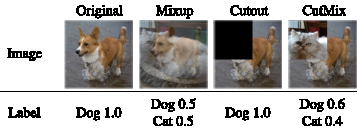
\includegraphics[width=0.9\linewidth]{images/augmentation.pdf}
    \caption{Different data augmentation methods with corresponding image labels.~\cite{Yun2019}}
    \label{fig:augment}
\end{figure}

Training samples can also be mixed or otherwise augmented in a feature space rather than directly in the input space. Neural networks, particularly autoencoders, can map images to low-dimensional feature representations, which can then be used for feature space augmentation. Synthetic instances are generated by manipulating the feature representations using methods such as adding noise or nearest neighbor interpolation and extrapolation.

Another oversampling strategy for dataset expansion is generative modeling, which can create artificial instances with characteristics similar to images from the training dataset. Generative Adversarial Networks (GANs)~\cite{Goodfellow2014} provide a framework for generative modeling through adversarial training, learning to create synthetic samples from the training data distribution. Various modifications can be applied to GANs that improve the quality of generated instances, which are then used to augment the training dataset.~\cite{Shorten2019, Yang2023}

\paragraph{} The choice of augmentation strategy determines the effective size of the training dataset. Multiple augmentation methods can be combined, but there is no established consensus on the optimal selection and combination of these methods or on the sufficient size of the final dataset. Augmentations can be applied online, generating new samples during training at the cost of additional computation but with minimal storage requirements, or offline, with augmented images created beforehand to reduce training time at the expense storage.

Data can also be augmented during inference using \textbf{test-time augmentation}, which averages predictions over multiple augmented versions of a test image to produce more robust neural network output. This approach can also improve uncertainty estimation, reducing highly confident but incorrect predictions. Test-time augmentation is analogous to ensemble learning in the data space, trading increased inference cost for improved predictions.~\cite{Shorten2019, Yang2023}


\section{Transfer Learning}
CNNs typically require a large amount of labeled training data to achieve good performance, and data augmentation or other regularization methods are often insufficient to prevent overfitting to small training datasets. Transfer learning allows deep neural networks to be trained on tasks with smaller datasets by \textbf{pre-training} them on a large dataset and then transferring the learned features to the target task. CNNs are commonly pre-trained on the ImageNet dataset, after which the learned features can be transferred either to the same computer vision task with a different dataset or to a different but related task such as object detection or image segmentation~\cite{Kornblith2019}. This approach leverages the knowledge acquired during pre-training to improve performance on the target task and significantly reduces the amount of labeled data required for effective training.~\cite{Krichen2023}

During transfer learning, the parameter values of the first $n$ layers of a pre-trained network are copied to the corresponding layers of the target network, while the remaining layers are initialized randomly. CNNs trained on image data tend to learn very similar first-layer features, which commonly occur regardless of the specific task or training dataset. These features are considered general, as they appear consistently in different training setups. In contrast, deeper layers capture increasingly task-specific features. General features are particularly suitable for transfer learning because they can be efficiently adapted to a wide range of tasks.

After transferring the pre-trained parameters, the randomly initialized layers of the target network are trained for the target task. During training, errors can also be backpropagated into the pre-trained layers to adapt them to the new domain. This is referred to as \textbf{fine-tuning}, which can improve performance on the target task, but may lead to overfitting if the target dataset is too small or the number of parameters is too large. Alternatively, the pre-trained layers can be frozen during training, effectively serving as fixed feature extractors for the remaining layers.

Pre-training almost any number of layers in a network has been shown to improve generalization performance when followed by fine-tuning to the target task. CNN pre-training on ImageNet can accelerate training convergence by an order of magnitude, even when the final performance is similar to training from scratch~\cite{Kornblith2019}. Transfer learning therefore enables faster training and better generalization, while preventing deep neural networks from overfitting to small datasets.~\cite{Yosinski2014}


\section{CNN Architectures}
AlexNet was the first CNN to significantly outperform traditional computer vision methods on the ImageNet dataset. Its architecture consists of five convolutional layers followed by three fully connected layers, as illustrated in Figure~\ref{fig:alexnet}, with ReLU activation applied after each hidden layer. The first two convolutional layers use kernel sizes of $11 \times 11$ and $5 \times 5$, respectively, and are followed by overlapping max pooling layers. The remaining convolutional layers employ $3 \times 3$ kernels, with the last one also followed by max pooling. To reduce overfitting, AlexNet applies dropout in the fully connected layers and uses random cropping and horizontal flipping for data augmentation.~\cite{Krizhevsky2012}

Following the success of AlexNet, numerous CNN architectures were proposed, introducing further improvements and making substantial contributions to the field of computer vision. These architectures vary widely in size and computational complexity, while consistently achieving higher classification accuracy on the ImageNet benchmark, as illustrated in Figure~\ref{fig:cnn_architectures}. The primary trend among these models is their increasing depth, enabled by newly introduced architectural and training techniques that make the optimization of deeper networks feasible.~\cite{Szeliski2022, Krichen2023}

\begin{figure}
    \centering
    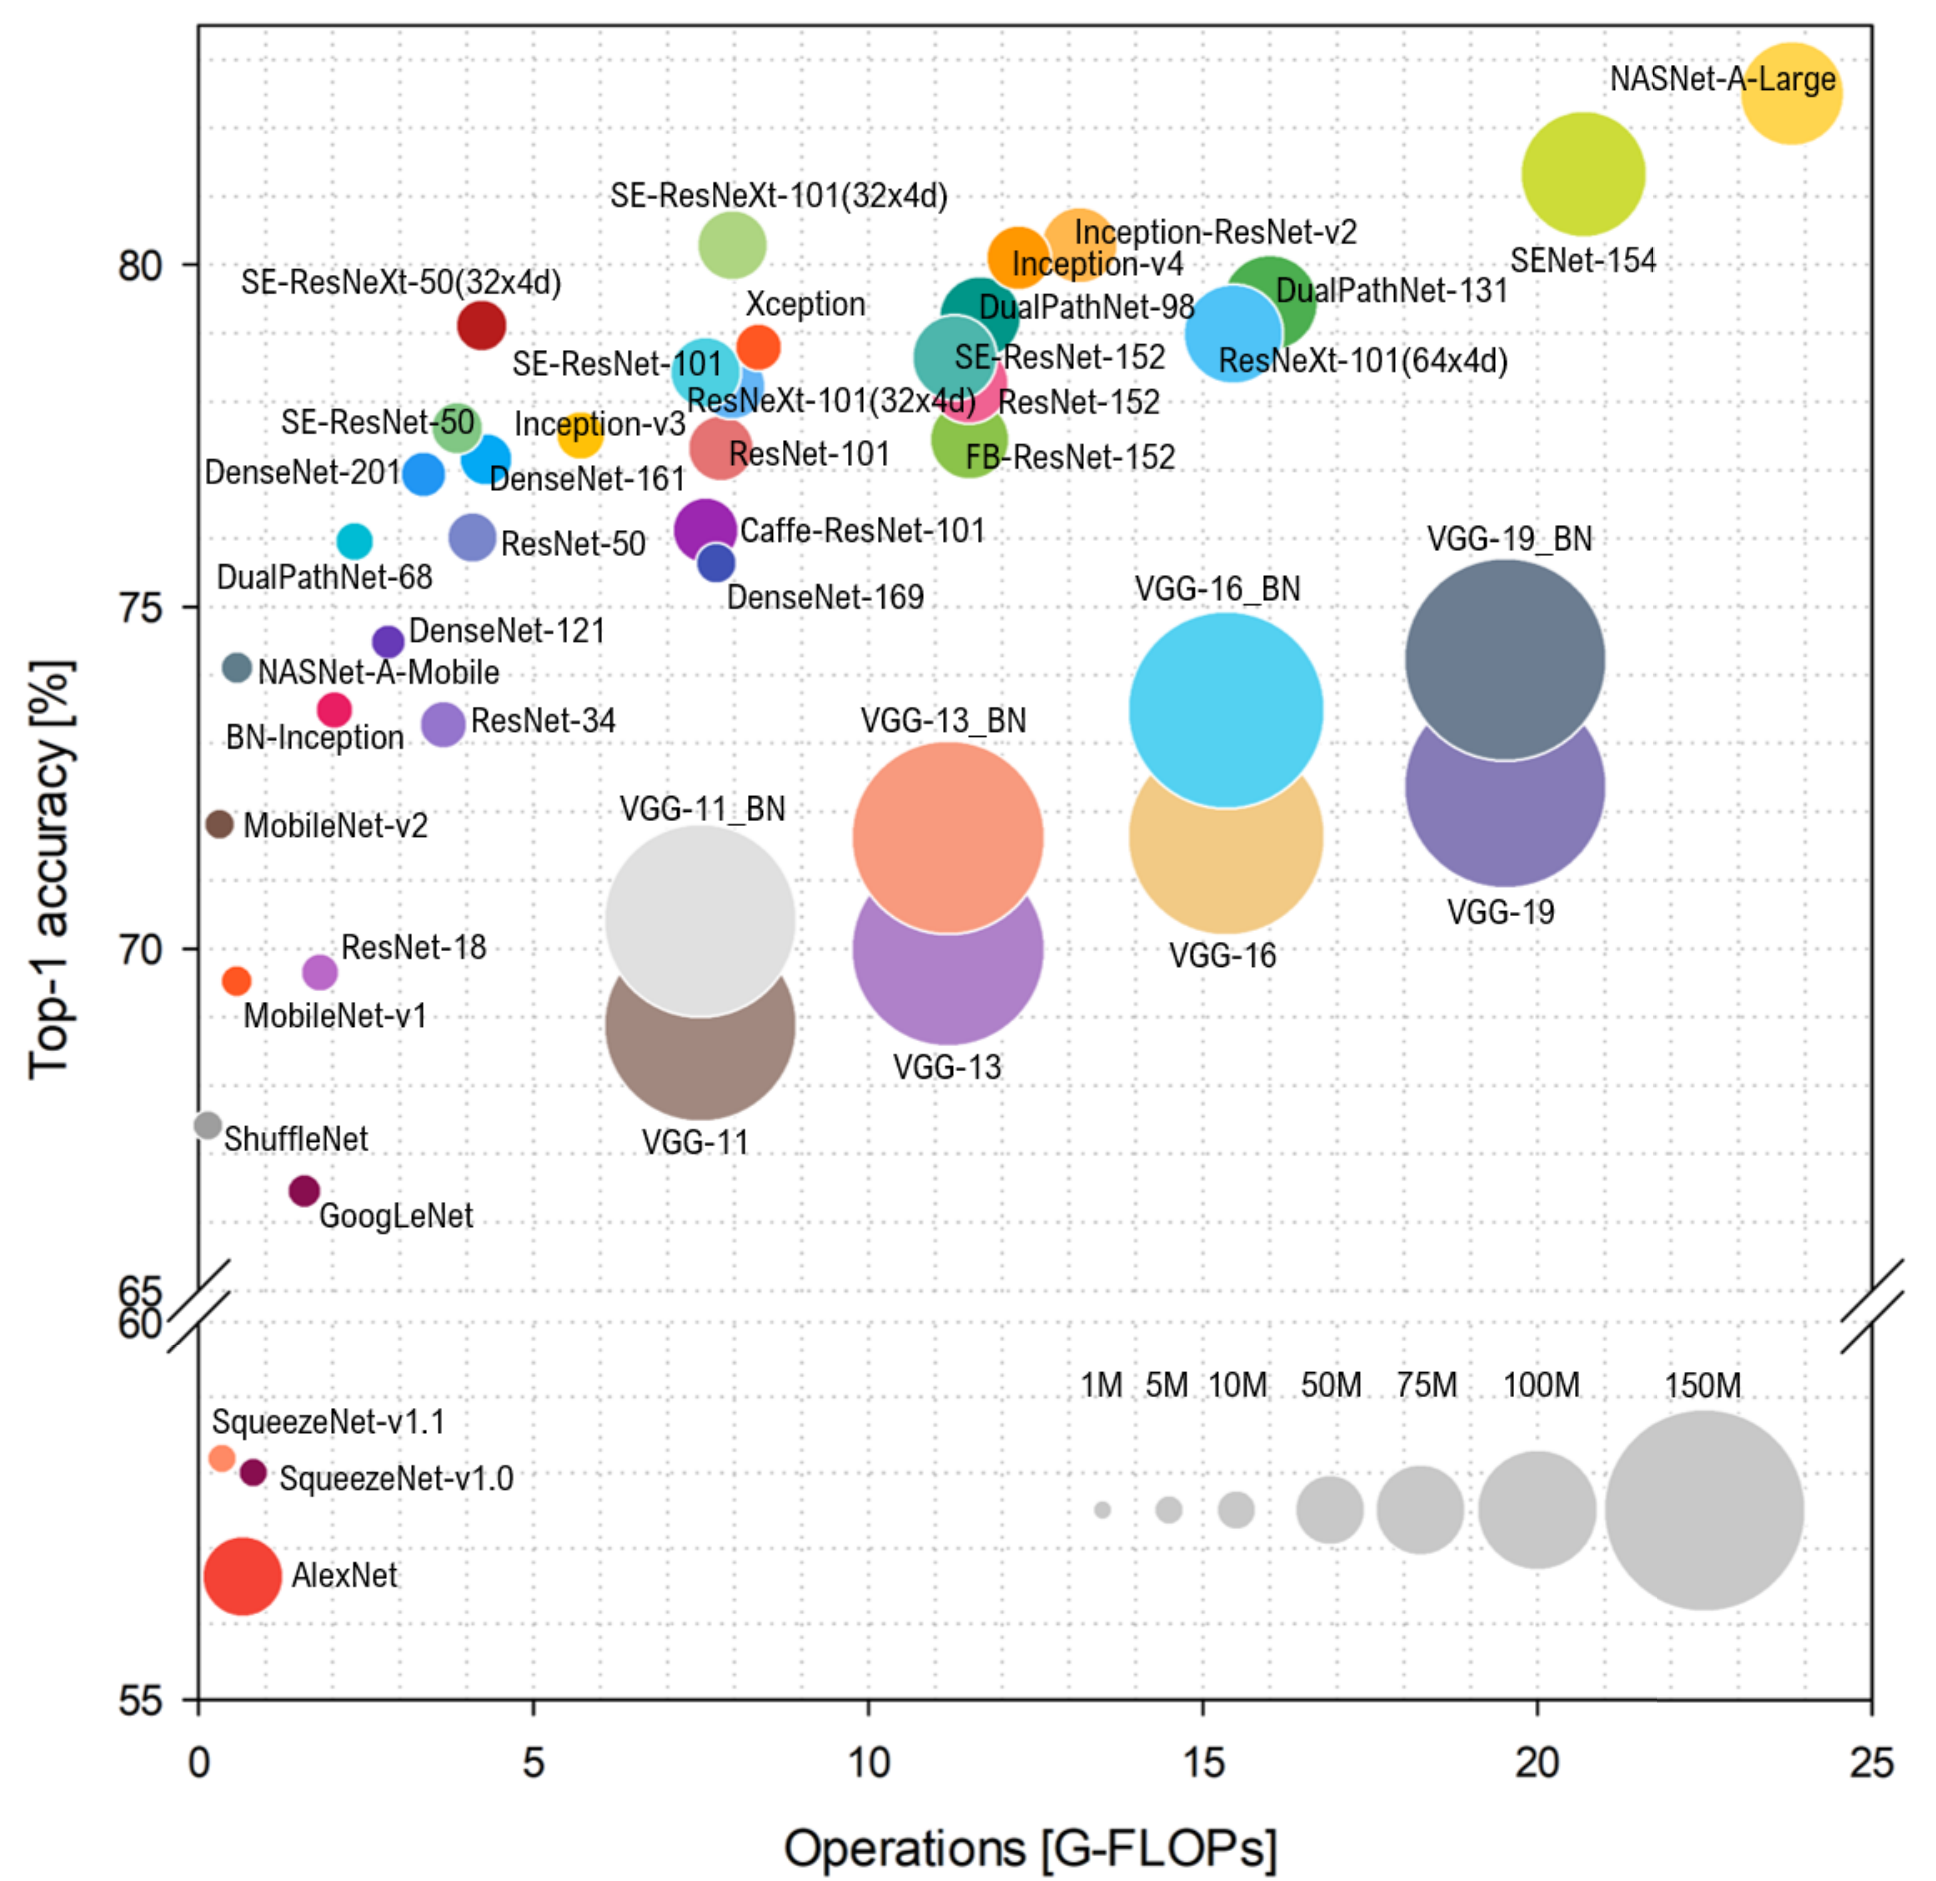
\includegraphics[width=0.6\linewidth]{images/cnn_architectures.png}
    \caption{Ball chart showing the top-1 accuracy on ImageNet with respect to the computational complexity measured by the number of floating point operations required for a single forward pass. The size of each ball corresponds to the number of parameters of each model.~\cite{Bianco2018}}
    \label{fig:cnn_architectures}
\end{figure}

\subsection{VGG} CNNs contain many hyperparameters that can be tuned to improve performance compared to the conventional architecture of AlexNet. The VGG (Visual Geometry Group) architecture~\cite{Simonyan2015} was developed to investigate the effect of CNN depth on its accuracy. It consists of a stack of convolutional layers followed by three fully connected layers, with the total depth depending on the specific VGG configuration and reaching up to 19 layers. All hidden layers use ReLU activation and five of the convolutional layers are followed by max pooling over a $2 \times 2$ pixel window with stride 2.

The increased depth is made possible by the use of very small $3 \times 3$ convolution filters with stride 1 throughout the entire network. This design simplifies the architecture and reduces the total number of parameters. Stacking multiple convolutional layers with small filters is effectively equivalent to using a single layer with a larger filter, but it introduces additional nonlinearities. For example, a stack of three $3 \times 3$ convolutions has a $7 \times 7$ receptive field but is more discriminative than a single $7 \times 7$ convolution due to the additional nonlinearities. The increased depth of VGG has been shown to improve accuracy, highlighting the importance of network depth for learning visual representations.~\cite{Simonyan2015}

\subsection{Inception} The aim of the Inception architecture~\cite{Szegedy2015} is to approximate an optimal sparse local structure using convolutional building blocks. This design allows increasing the depth and width of the network while keeping computational complexity under control. Inception achieves this by using parallel convolutions of different sizes, enabling the extraction of features at multiple scales simultaneously. An Inception module, shown in Figure~\ref{fig:inception}~(a), combines $1 \times 1$, $3 \times 3$, and $5 \times 5$ convolutions along with a $3 \times 3$ max pooling and aggregates their outputs by concatenating the channels to preserve multi-scale information.

Directly stacking these modules would quickly become inefficient because the number of channels would keep increasing throughout the networks. Even a small number of $5 \times 5$ convolutions would become too expensive, causing computational bottlenecks that would limit the overall size of the network. To address this and reduce the number of channels, $1 \times 1$ convolutions are inserted before the more expensive $3 \times 3$ and $5 \times 5$ convolutions and after the max pooling, as shown in Figure~\ref{fig:inception}~(b). These convolutions do not perform any spatial aggregation due to their filter size and instead act as linear projections across channels to reduce dimensionality. This architecture allows controlling the number of channels in each layer of the network and introduces additional ReLU activations after the $1 \times 1$ convolutions.

\begin{figure}
    \centering
    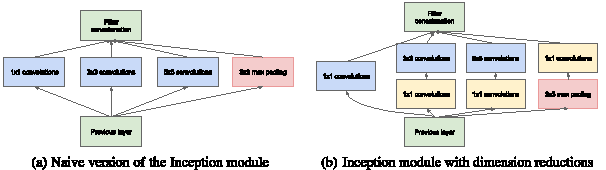
\includegraphics[width=\linewidth]{images/inception.pdf}
    \caption{Inception module.~\cite{Szegedy2015}}
    \label{fig:inception}
\end{figure}

An Inception network is built by stacking these modules, with occasional max pooling layers with stride 2 to reduce the spatial resolution of feature maps. \textbf{GoogLeNet} is a specific instance of the Inception architecture with 22 weight layers. It begins with two standard convolutional layers separated by a max pooling layer, followed by a sequence of Inception modules. All convolutions, including those inside the modules, use ReLU activations, and a global average pooling layer is used before one final fully connected layer. During training, two small auxiliary CNN classifiers are attached to intermediate layers to prevent vanishing gradients while providing additional regularization.~\cite{Szegedy2015}

\subsection{ResNet} Network depth has been shown to be a crucial factor in CNN performance. However, deeper networks are more difficult to train. The vanishing gradient problem, which previously prevented deeper networks from converging, has largely been mitigated through careful weight initialization, ReLU activations, and batch normalization. This has revealed the degradation problem, where increasing network depth leads to accuracy saturation followed by rapid degradation. This behavior is not caused by overfitting, as deeper models also lead to higher training errors.

The deep residual learning framework addresses the degradation problem to enable the training of very deep networks. A building block of a residual network consists of several stacked layers with a shortcut connection. If $\mathcal{H}(\mathbf{x})$ denotes the optimal underlying mapping of a stack of layers with input $\mathbf{x}$, each building block approximates a residual function $\mathcal{F}(\mathbf{x}) = \mathcal{H}(\mathbf{x}) - \mathbf{x}$ and computes the output $\mathcal{F}(\mathbf{x}) + \mathbf{x}$ using an identity shortcut connection and element-wise addition, as shown in Figure~\ref{fig:resnet}. Identity shortcut connections are sufficient to address the degradation problem and introduce no additional parameters or computational complexity. When the dimensions of $\mathbf{x}$ and $\mathcal{F}(\mathbf{x})$ differ, projection shortcut connections are used instead of identity. Linear projection shortcuts are implemented by $1 \times 1$ convolutions with stride 2 to match both channel number and feature map resolution.

\begin{figure}
    \centering
    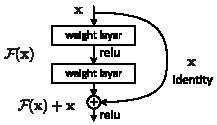
\includegraphics[width=0.5\linewidth]{images/resnet.pdf}
    \caption{Building block of a residual network.~\cite{He2016}}
    \label{fig:resnet}
\end{figure}

The ResNet architecture~\cite{He2016} follows the strategy of VGG, relying primarily on $3 \times 3$ convolutions with an increasing number of channels. The network begins with a $7 \times 7$ convolution and a max pooling layer, followed by a sequence of residual building blocks. To reduce computational complexity, ResNet uses a bottleneck block design, which consists of a $3 \times 3$ convolution preceded and followed by $1 \times 1$ convolutions that reduce and subsequently restore the number of channels. Spatial subsampling is performed using convolutions with a stride of 2 within selected residual blocks. Batch normalization is applied after each convolution, and the network ends with a global average pooling layer followed by a single fully connected layer.

A 152 layer ResNet achieves excellent performance on ImageNet while maintaining lower computational complexity than VGG due to the bottleneck design and the use of fewer channels throughout the architecture. The \textbf{ResNeXt} architecture~\cite{Xie2017} further extends ResNet by splitting residual blocks into multiple parallel branches inspired by the Inception module. Because all branches share the same topology, this design is equivalent to grouped convolutions and improves the network accuracy without increasing computational complexity.~\cite{He2016}

\subsection{EfficientNet} CNN architectures are commonly partitioned into multiple stages, where all layers within each stage share the same structure. Transitions between stages are typically realized by layers that reduce the spatial resolution of feature maps and change the network width, which is defined as the number of channels in each layer. CNNs can be scaled up to achieve better accuracy, most commonly by increasing the network depth, width, or input resolution without modifying the underlying architecture. EfficientNet~\cite{Tan2019} introduced a compound scaling method that uniformly scales all these dimensions using a single compound coefficient.

Conventional methods scale CNNs along only one of these dimensions, which results in diminishing accuracy gains as model size increases. Multiple dimensions can be arbitrarily scaled together, but this requires manual tuning and often yields suboptimal results because the optimal values of depth, width, and resolution are interdependent and vary under different computational constraints. Intuitively, CNNs with higher-resolution inputs require more layers to sufficiently expand the receptive field, as well as more channels to capture more fine-grained patterns. This suggests that different scaling dimensions must be carefully balanced to achieve optimal performance gains.

The baseline EfficientNet architecture was designed using neural architecture search to jointly optimize accuracy and computational complexity with balanced trade-off. Its core building block is the inverted residual bottleneck with depthwise convolutions, adopted from MobileNetV2~\cite{Sandler2018}, with squeeze-and-excitation blocks~\cite{Hu2020}. The baseline network is then scaled using the compound scaling method that aims to maximize model accuracy under a given computational resource constraint controlled by a compound coefficient. It uniformly scales the network depth, width, and resolution according to a fixed ratio determined through a small grid search. The compound scaling method further improves accuracy compared to single-dimension scaling methods, allowing EfficientNet models to outperform other CNNs while using significantly fewer parameters.~\cite{Tan2019}

\subsection{ConvNeXt} With the emergence of vision transformers, CNNs have been largely replaced as the state-of-the-art computer vision model. The Vision Transformer~\cite{Dosovitskiy2021}, when trained with sufficient model capacity on large datasets, significantly outperformed standard ResNet models in image classification. The hierarchical Swin Transformer~\cite{Liu2021} further reintroduced several image-specific CNN priors and achieved state-of-the-art performance across a wide range of computer vision tasks beyond classification.

ConvNeXt~\cite{Liu2022} was proposed to systematically examine the CNN design space and evaluate the performance limits of pure convolutional architectures. It gradually modernizes a ResNet baseline by incorporating design choices inspired by hierarchical vision transformers without introducing any attention mechanisms. The resulting network consists exclusively of standard CNN components and maintains the architectural simplicity of pure CNNs, while competing favorably with vision transformers in terms of accuracy, scalability, and robustness across major benchmarks, as shown in Figure~\ref{fig:convnext}.

\begin{figure}
    \centering
    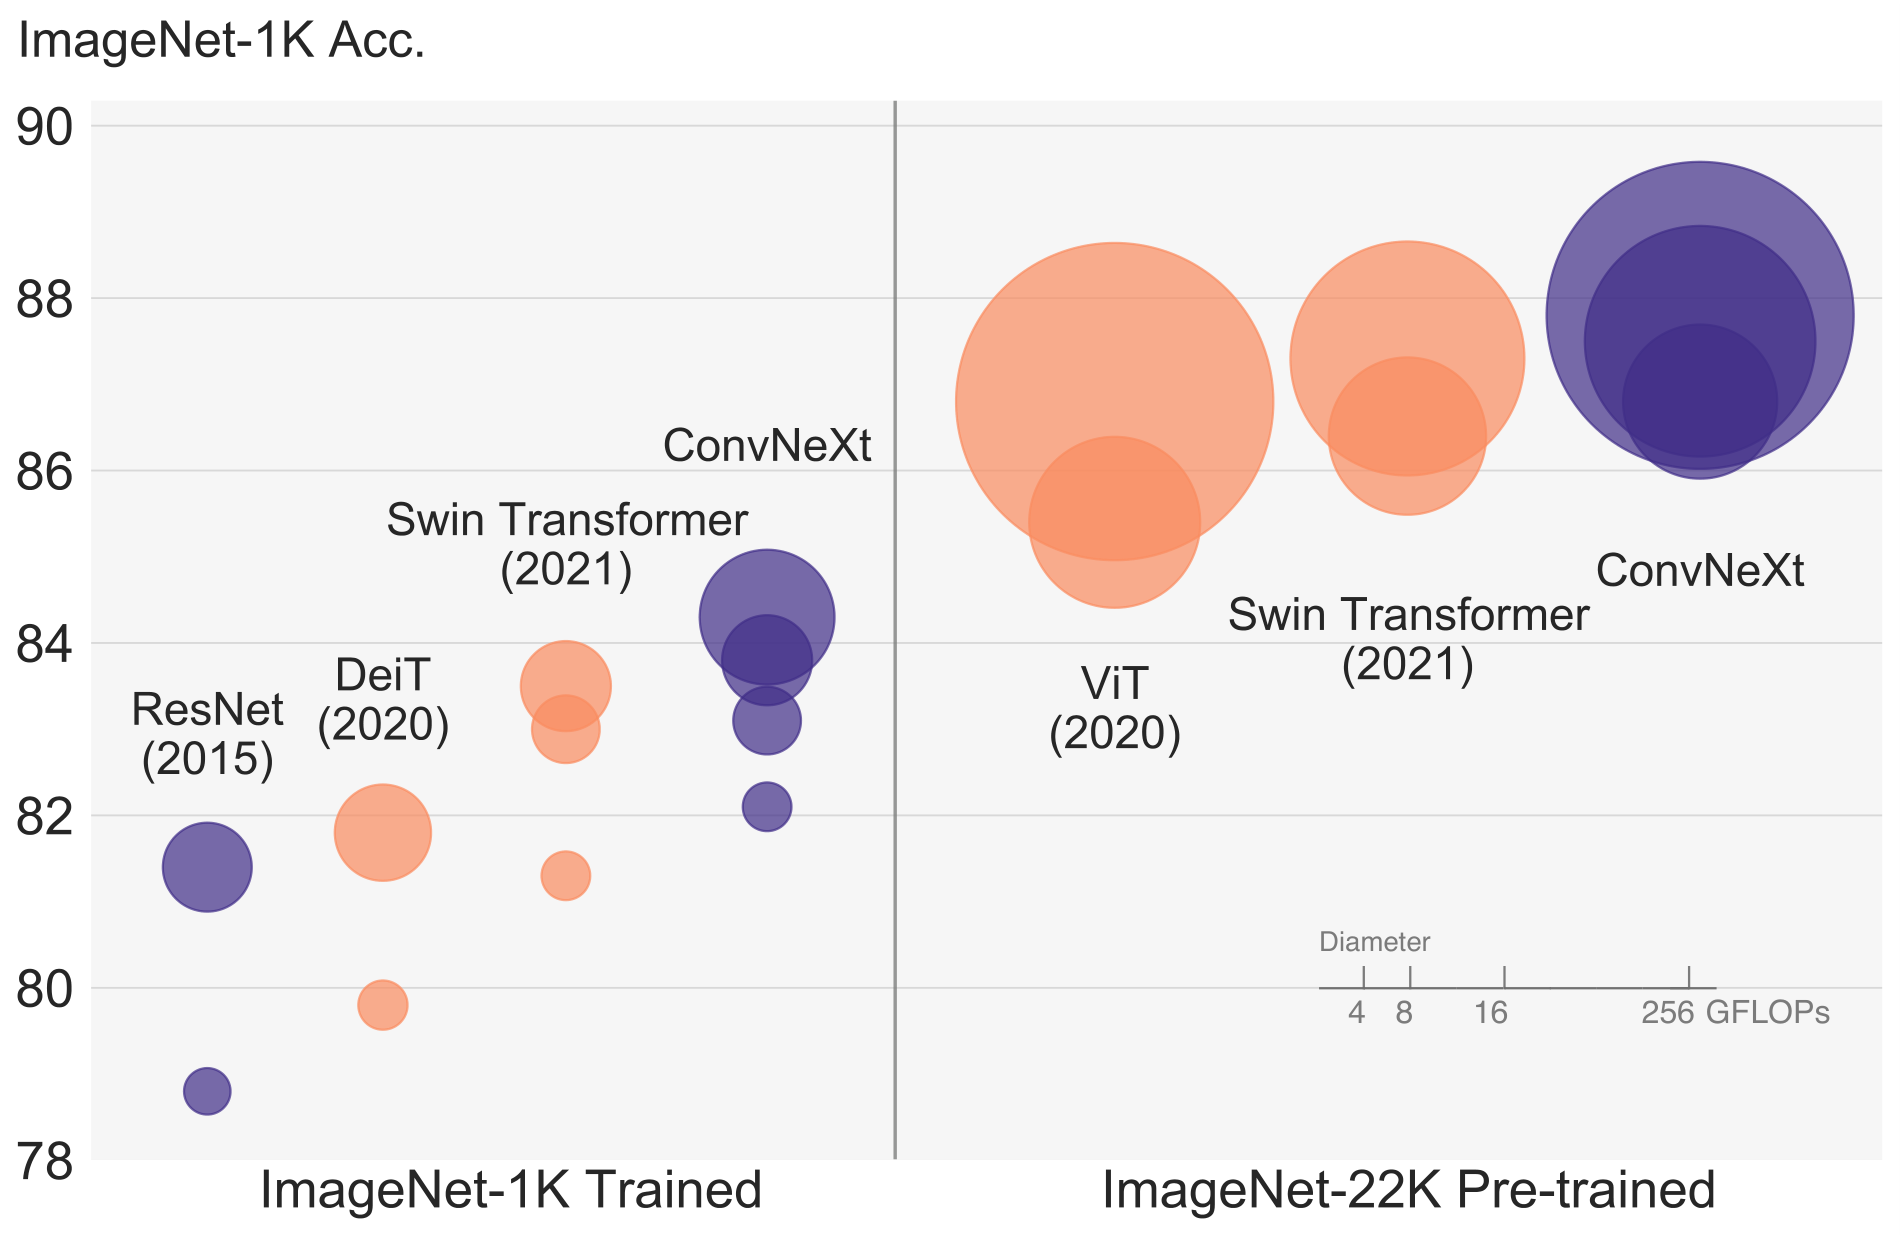
\includegraphics[width=0.64\linewidth]{images/convnext.png}
    \caption{Ball chart comparing ImageNet-1K classification accuracy of CNNs and vision transformers. ResNet and ViT results are obtained with improved training strategies. Each model family is represented by multiple scaled variants also distinguished by their ImageNet training approach. The size of each ball corresponds to the computational complexity of the model.~\cite{Liu2022}}
    \label{fig:convnext}
\end{figure}

The ConvNeXt architecture is derived from a ResNet model trained using optimization strategies commonly adopted for vision transformers, differing primarily in the chosen optimizer and associated hyperparameter settings. The network is then incrementally modified to improve performance while controlling computational complexity. The most notable change is a redesigned residual block, which enables increasing network width and expanding the standard $3 \times 3$ convolutions to $7 \times 7$. Additional modifications include the use of separate convolutional layers for spatial subsampling, replacing ReLU activations with Gaussian Error Linear Unit (GELU) activations~\cite{Hendrycks2023}, substituting batch normalization with layer normalization~\cite{Ba2016}, and reducing the number of activation and normalization layers within each block of the network.~\cite{Liu2022}



\chapter{CNN Architectures for Object Detection}
Before the introduction of CNNs to image classification, object detection performance had plateaued, with the best-performing approaches relying on complex ensemble systems that combined low-level features with high-level contextual information~\cite{Girshick2014}. An exhaustive search can be used to adapt classification models for object detection by applying them at every possible location and scale within an image, but it is very inefficient and prone to errors. A more effective solution is to design specialized detectors that can quickly identify regions likely to contain objects of interest.

This is the approach used by two-stage object detectors. In the first stage, a region proposal algorithm generates a set of candidate regions within the input image, which are then classified in the second stage to evaluate the presence of any objects. A CNN backbone is used for feature extraction, and one or more detection heads operate on the extracted features to classify each proposed region, produce confidence scores, and further refine the detections. One-stage object detectors are architecturally similar, but unify the proposal and classification stages into a single CNN that directly produces all detections in the image with a single forward pass through the network.~\cite{Szeliski2022, Liu2020}


\section{R-CNN}
Regions with CNN features (R-CNN)~\cite{Girshick2014} is a two-stage detection system that bridges the gap between image classification and object detection by combining region proposals with CNNs, as illustrated in Figure~\ref{fig:rcnn}. During inference, R-CNN extracts approximately 2000 class-independent region proposals from each input image using the selective search algorithm~\cite{Uijlings2013}. Each proposal, regardless of its shape or size, is rescaled to a fixed spatial resolution and forward propagated through an AlexNet~\cite{Krizhevsky2012} backbone to extract features. AlexNet produces a 4096-dimensional feature vector from its penultimate fully connected layer for each proposal. The extracted features are then classified using a separate linear Support Vector Machine (SVM)~\cite{Cortes1995} for each class.

The localization performance of R-CNN is further improved through class-specific bounding box regression, which refines the proposed bounding boxes using predicted scale and translation offsets. These offsets are modeled as linear functions of features produced by the last pooling layer of the backbone, with the function parameters learned using ridge regression with strong regularization. Finally, greedy \textbf{Non-Maximum Suppression (NMS)} is applied independently for each class to remove duplicate detections. A detection is removed if it has an $\text{IoU} \ge \tau$ overlap with any higher-confidence prediction of the same class, where $\tau$ is a fixed threshold.~\cite{Girshick2014}

\begin{figure}
    \centering
    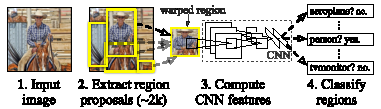
\includegraphics[width=0.9\linewidth]{images/rcnn.pdf}
    \caption{R-CNN two-stage detection pipeline.~\cite{Girshick2014}}
    \label{fig:rcnn}
\end{figure}

\paragraph{Region proposal} R-CNN uses the selective search algorithm, which combines image segmentation with exhaustive search, to generate region proposals. Selective search uses bottom-up hierarchical grouping with a diverse set of similarity measures designed to capture a wide variety of objects. An image is first segmented into a set of initial regions, which are then iteratively merged based on their similarity. This naturally captures objects at all scales, while the use of complementary similarity measures and color spaces provides robustness to varying image conditions. As a result, selective search produces a set of high-quality, class-independent region proposals with very high recall.~\cite{Uijlings2013}

The proposed regions are of arbitrary shape and size, while AlexNet requires a fixed-size $227 \times 227$ input. R-CNN encloses each region within a tight rectangular bounding box and anisotropically scales it to the target resolution, regardless of its original aspect ratio. Prior to scaling, each proposal is padded with additional image context, so that it contains exactly 16 pixels of context around the original proposal at the scaled resolution. This padding has been shown to improve detection performance.~\cite{Girshick2014}

\paragraph{Training} R-CNN uses transfer learning to prevent overfitting to smaller object detection datasets. The AlexNet backbone is pre-trained on the ImageNet classification dataset and subsequently fine-tuned on generated region proposals to adapt it to the detection task. During fine-tuning, the final classification layer is replaced with a randomly initialized $(C + 1)$-dimensional layer corresponding to $C$ object classes and one background class. Each region proposal in the training dataset is matched to the ground truth bounding box with the highest IoU overlap and is labeled as positive for that class if $\text{IoU} \ge 0.5$. Otherwise, it is labeled as background and serves as a negative example for all classes. The sampling of training data is biased towards positive instances, which are otherwise vastly outnumbered by background region proposals.

This definition of positive and negative instances for fine-tuning is chosen to increase the number of positives in the training dataset. It introduces many jittered samples, effectively serving as a form of data augmentation, expanding the dataset and preventing overfitting. This allows the backbone to learn sufficiently discriminative features, but is suboptimal for precise localization. For this reason, R-CNN replaces the fine-tuned softmax classifier with class-specific SVMs for the final classification. The SVMs are trained using only ground truth bounding boxes as positive instances, which emphasizes accurate localization. Region proposals with $\text{IoU} \le 0.3$ relative to all ground truth instances of a given class are treated as negatives, and the rest are ignored.~\cite{Girshick2014}

\subsection{Fast R-CNN}
The main drawback of R-CNN is its expensive training and slow inference, caused by separate feature extraction for each region proposal without any shared computation. Its training pipeline is also complicated, as it consists of three separately trained stages. Fast R-CNN~\cite{Girshick2015} introduces a new training approach that jointly optimizes the classification and bounding box regression heads using a multi-task loss, updating all network layers simultaneously. This speeds up both training and inference while also improving detection accuracy.

Fast R-CNN uses a VGG-16~\cite{Simonyan2015} backbone to process the entire input image together with a set of generated region proposals. The image is forward propagated through the backbone, with the last pooling layer replaced by a Region of Interest (ROI) pooling layer. ROI pooling rescales each ROI, which is a rectangular window in the feature map corresponding to a projected region proposal, at the feature level instead of rescaling region proposals at the image level before forward propagation. The ROI pooling layer converts each ROI into a fixed-size $H \times W$ feature map by dividing it into a $H \times W$ grid of sub-windows and applying max pooling within each cell. The values of $H$ and $W$ are chosen to be compatible with the following fully connected layers.

The resulting ROI feature maps are processed by the fully connected layers of the CNN backbone to extract a fixed-length feature vector for each region proposal, as shown in Figure~\ref{fig:fast_rcnn}. The final fully connected layer with softmax classifier is replaced by two parallel output layers. The first classifies the feature vector into $C + 1$ classes, while the second predicts the bounding box regression offsets for each of the $C$ object classes. Only the offsets corresponding to the predicted class are used to refine the bounding box positions.~\cite{Girshick2015}

\begin{figure}
    \centering
    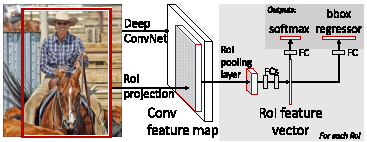
\includegraphics[width=0.7\linewidth]{images/fast_rcnn.pdf}
    \caption{Fast R-CNN architecture.~\cite{Girshick2015}}
    \label{fig:fast_rcnn}
\end{figure}

\paragraph{Multi-task training} Fast R-CNN is trained end-to-end in a single fine-tuning stage that jointly optimizes both output layers using a multi-task loss. This unified training avoids the complicated R-CNN pipeline and allows the classification and localization tasks to influence each other through shared representation. For a region proposal with ground truth class $u$ and bounding box regression target $t$, the network predicts a class probability distribution $\hat{p}$ and a tuple of bounding box offsets $\hat{t}_k$ for each class $k$. The multi-task loss is defined as:
\begin{equation}\label{eq:rcnn}
    L(u, \hat{p}, t, \hat{t}_u) = L_{CCE}(u, \hat{p}) + \lambda[u \ge 1]L_{LOC}(t, \hat{t}_u)
\end{equation}
where $L_{CCE}$ is the categorical cross-entropy loss for classification, defined in Equation~\ref{eq:cce}, and $L_{LOC}$ is the smooth $L_1$ localization loss. The indicator function $[u \ge 1]$ disables the localization loss for background region proposals labeled $u = 0$ and $\lambda$ controls the balance between the two losses.

During training, positive instances are sampled from region proposals with $\text{IoU} \ge 0.5$ overlap with a ground truth bounding box, while negative instances are sampled from proposals whose maximum IoU with any ground truth bounding box lies in the interval $[0.1, 0.5)$. The lower threshold 0.1 serves as a heuristic for hard negative mining, selecting the most challenging negative instances. Minibatches are sampled hierarchically by first selecting a small number of images and then drawing multiple region proposals from each image, enabling shared computation and memory usage.~\cite{Girshick2015}

\subsection{Faster R-CNN}
Fast R-CNN significantly increased detection speed by sharing convolutions across region proposals, which exposed a new computational bottleneck caused by the external region proposal algorithm. Faster R-CNN~\cite{Ren2015} addresses this issue by replacing selective search with a Region Proposal Network (RPN), creating a single unified network for object detection that can be trained end-to-end. The RPN generates a set of high-quality rectangular region proposals, which are then processed by the standard Fast R-CNN object detector. Additionally, RPN shares convolutional features with Fast R-CNN, which allows region proposal computation at almost no additional cost.

The RPN is constructed on top of the last shared convolutional layer of the Fast R-CNN backbone. It uses an $n \times n$ sliding window over the convolutional feature maps to predict $k$ region proposals at each spatial location. Each of the $k$ proposals is predicted relative to one of $k$ predefined anchor boxes centered at the window position and associated with a specific scale and aspect ratio. Anchors ensure translation invariance of region proposals and enable efficient handling of objects at multiple scales. The sliding window serves as input to a fully connected layer, followed by two parallel output layers for region classification and bounding box regression. Because the fully connected layers are shared across all spatial locations of the feature map, the RPN can be implemented as a fully convolutional network, using an $n \times n$ convolution followed by two parallel $1 \times 1$ convolutional output layers.

For each region proposal, the output layers predict an objectness score, which represents the confidence that the region contains an object rather than background, and four bounding box regression offsets relative to the corresponding anchor box. Each of the $k$ anchors is associated with a separate bounding box regressor to predict regions of various sizes. Each regressor is responsible for a specific scale and aspect ratio, and the $k$ regressors do not share weights. After prediction, all region proposals extending beyond the image boundary are clipped, and NMS removes redundant overlapping proposals based on their objectness scores. NMS substantially reduces the number of proposals without harming detection accuracy. Finally, the top-N region proposals ranked by objectness are classified by Fast R-CNN.~\cite{Ren2015}

\paragraph{Alternating training} The RPN and Fast R-CNN share a set of convolutional layers, but update them differently during training. Faster R-CNN trains them together using an alternating four-step algorithm to learn shared features. First, an RPN pre-trained on ImageNet is fine-tuned for the region proposal task. Then a separate Fast R-CNN pre-trained on ImageNet is fine-tuned using the proposals generated by the RPN. In the third step, the RPN is initialized with the Fast R-CNN backbone, freezing the shared convolutional layers while fine-tuning the rest. Lastly, with shared features established, the backbone is kept frozen, and the remaining Fast R-CNN layers are fine-tuned again.

The RPN is trained using the same multi-task loss as Fast R-CNN, defined in Equation~\ref{eq:rcnn}. The classification loss evaluates the objectness score, and the localization loss evaluates the anchor bounding box regression, which is disabled for background anchors. During training, anchor boxes that cross image boundaries are ignored, and the remaining anchors are assigned binary labels. Anchors with the highest IoU overlap with a ground truth bounding box or anchors with $\text{IoU} \ge 0.7$ overlap with any ground truth bounding box are labeled positive, and non-positive anchors with $\text{IoU} \le 0.3$ overlap with all ground truth boxes are labeled negative, while the remaining anchors do not contribute to the training objective.~\cite{Ren2015}


\section{YOLO}
You Only Look Once (YOLO)~\cite{Redmon2016} is a one-stage object detection CNN that reframes detection as a regression problem. It uses features from the entire input image to directly predict all bounding boxes and their class probabilities in a single forward pass. This design enables real-time inference while maintaining high detection performance. By reasoning globally about the image, YOLO produces significantly fewer background errors compared to Fast R-CNN, which relies on local region proposals and often mistakes background regions for objects.

The YOLO architecture is inspired by GoogLeNet~\cite{Szegedy2015} and consists of 24 convolutional layers followed by 2 fully connected layers, with the Inception modules replaced by bottleneck blocks containing $1 \times 1$ and $3 \times 3$ convolutions. YOLO divides the input image into an $S \times S$ grid, and each grid cell predicts $B$ bounding boxes whose centers fall within that cell. The bounding boxes are predicted using a fully connected regression output layer arranged in an $S \times S \times (B \cdot 5 + C)$ tensor. Each bounding box is represented by coordinates $(x, y, w, h)$ and an objectness score $o$, where $(x, y)$ represent the center relative to the grid cell boundaries, and the width $w$ and height $h$ are parametrized relative to the dimensions of the full image. The objectness $o$ is defined as $\operatorname{Pr}(\text{object}) \cdot \text{IoU}(b, \text{object})$, combining the confidence that the bounding box contains an object with its localization accuracy.

\begin{figure}[!b]
    \centering
    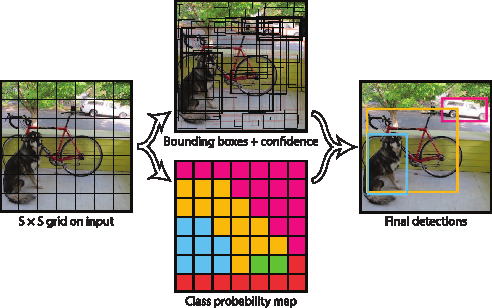
\includegraphics[width=0.8\linewidth]{images/yolo.pdf}
    \caption{YOLO detection process in a single unified network. The image is divided into an $S \times S$ grid and each cell predicts bounding boxes with objectness scores (confidences) and conditional class probabilities. The final detections are obtained by multiplying the objectness scores with the class probabilities.~\cite{Redmon2016}}
    \label{fig:yolo}
\end{figure}

YOLO also predicts $C$ conditional class probabilities $\operatorname{Pr}(\text{class}_i \mid \text{object})$ for each grid cell, shared across all bounding boxes within that cell. During inference, objectness scores are multiplied by these conditional probabilities to obtain class-specific confidences, as illustrated in Figure~\ref{fig:yolo}. Although YOLO often predicts a single bounding box per object, NMS can be applied to remove duplicate detections and further improve performance.~\cite{Redmon2016}

\paragraph{Training} YOLO is trained end-to-end on full images, directly optimizing detection performance. The backbone is pre-trained on ImageNet and then converted for object detection by adding four convolutional layers and two fully connected layers with randomly initialized weights. The network is fine-tuned using input images of size $448 \times 448$, which is double the resolution used during pre-training.

During fine-tuning, each ground truth object is assigned to the bounding box with the highest current IoU overlap among predictions within the respective grid cell. This encourages specialization between the bounding box predictors for different object sizes, aspect ratios, and classes. YOLO optimizes a multi-part $L_2$ loss that combines bounding box localization, objectness, and classification terms:
\begin{equation}
\begin{split}
    E &= \lambda_{\text{coord}} \sum_{i = 0}^{S^2} \sum_{j = 0}^B \mathbbm{1}_{ij}^\text{obj} [(x_i - \hat{x}_i)^2 + (y_i - \hat{y}_i)^2] \\
    &\quad + \lambda_{\text{coord}} \sum_{i = 0}^{S^2} \sum_{j = 0}^B \mathbbm{1}_{ij}^\text{obj} [(\sqrt{w_i} - \sqrt{\hat{w}_i})^2 + (\sqrt{h_i} - \sqrt{\hat{h}_i})^2] \\
    &\quad + \sum_{i = 0}^{S^2} \sum_{j = 0}^B \mathbbm{1}_{ij}^\text{obj} (o_i - \hat{o}_i)^2 + \lambda_{\text{noobj}} \sum_{i = 0}^{S^2} \sum_{j = 0}^B \mathbbm{1}_{ij}^\text{noobj} (o_i - \hat{o}_i)^2 \\
    &\quad + \sum_{i = 0}^{S^2} \mathbbm{1}_i^\text{obj} \sum_{k \in \text{classes}} (p_i(k) - \hat{p}_i(k))^2
\end{split}
\end{equation}
where $(x_i, y_i, w_i, h_i)$, and $o_i$ are the ground truth bounding box coordinates and objectness scores, $p_i(k)$ is the probability of class $k$, and circumflexes denote the corresponding predictions. The indicator functions $\mathbbm{1}_{ij}^\text{obj}$ and $\mathbbm{1}_{ij}^\text{noobj}$ distinguish between object and background predictions by specifying whether an object appears in cell $i$ and is assigned to bounding box $j$. Only bounding boxes assigned a ground truth object contribute to the classification and localization loss.

The loss terms are balanced using the parameter values $\lambda_{\text{coord}} = 5$ and $\lambda_{\text{noobj}} = 0.5$, increasing the weight of localization errors and reducing the influence of background objectness errors. The square roots of bounding box width and height are predicted instead of their direct values, so small errors in large bounding boxes are penalized less than in small bounding boxes, where small errors matter more.~\cite{Redmon2016}

\subsection{YOLOv2 and YOLOv3}
Although YOLO is very fast, it makes a significant number of localization errors and has a relatively low recall compared to two-stage detectors. This is partly due to strong spatial constraints imposed on predictions, allowing each grid cell to predict only a fixed number of bounding boxes. While this reduces duplicate detections, it limits the number of nearby, especially small, objects that can be detected~\cite{Redmon2016}. YOLOv2~\cite{Redmon2017} and YOLOv3~\cite{Redmon2018} introduce a series of incremental updates to address these limitations, significantly improving performance while maintaining real-time inference. Although the resulting network struggles to predict perfectly aligned bounding boxes, it achieves high $\mathrm{AP}_{50}$ and performs relatively well on small objects.

YOLOv3 employs a significantly larger backbone called Darknet-53, which simplifies the architecture and adds shortcut connections. It consists of 53 convolutional layers with residual bottleneck blocks using $1 \times 1$ and $3 \times 3$ convolutions, replaces pooling layers with strided convolutions, and includes batch normalization to stabilize training. The complete YOLOv3 network is fully convolutional, as it removes fully connected layers from the original architecture and uses a $1 \times 1$ convolutional output layer to predict bounding boxes relative to a set of anchor boxes, similar to the RPN in Faster R-CNN~\cite{Ren2015}. With the transition to anchor boxes, class probabilities are decoupled from spatial location and predicted for each bounding box separately.

The network is still trained end-to-end on full images, pre-trained on ImageNet, and fine-tuned for object detection, with each ground truth bounding box assigned to a single anchor. Bounding box localization is trained using the $L_2$ loss, while objectness scores and class probabilities use binary cross-entropy. Class probabilities are predicted using $C$ independent binary classifiers instead of softmax, allowing multi-label classification. YOLOv3 is fully convolutional, so it can process images of different sizes. It learns to predict at multiple input resolutions using multi-scale training, where the input resolution changes every few iterations. This allows flexible scaling of the network during inference by increasing or decreasing the input image resolution.~\cite{Redmon2017, Redmon2018}

\paragraph{Anchor boxes} YOLOv3 no longer divides the input image into a fixed-size grid, which is instead defined based on the dimensions of the feature map extracted by the backbone. Bounding boxes are predicted at each spatial location of the feature map relative to predefined anchor boxes, which are chosen using k-means clustering on training bounding boxes with IoU similarity measure and 9 clusters divided evenly across 3 scales.

While the width $w$ and height $h$ of the bounding boxes are predicted as offsets from the anchor boxes, predicting the $(x, y)$ coordinates as unconstrained offsets can place bounding boxes anywhere in the image, regardless of the location of the corresponding anchor. This leads to training instability, so YOLOv3 predicts the $(x, y)$ coordinates relative to the boundaries of the respective grid cell, constrained by a sigmoid activation. This ensures that the center of each bounding box remains within its grid cell. Each prediction then consists of $t_x, t_y, t_w, t_h$, corresponding to the coordinates:
\begin{align}
    x &= \sigma(t_x) + c_x \\
    y &= \sigma(t_y) + c_y \\
    w &= p_w e^{t_w} \\
    h &= p_h e^{t_h}
\end{align}
where $(c_x, c_y)$ are the coordinates of the upper left corner of the respective grid cell, and $p_w$ and $p_h$ are the width and height of the anchor box. Using anchor boxes significantly increases the number of detections per image and simplifies the learning problem.~\cite{Redmon2017, Redmon2018}

\paragraph{Multi-scale detection} The low-resolution features extracted by the final backbone layer contain strong semantic information suitable for detecting larger objects, but the detection of smaller objects can benefit from higher-resolution features. YOLOv3 therefore predicts bounding boxes at three different scales, following an approach similar to feature pyramid networks~\cite{Lin2017}, which combine features from different scales into a feature pyramid using a top-down pathway and lateral connections, as illustrated in Figure~\ref{fig:fpn}.

\begin{figure}[b]
    \centering
    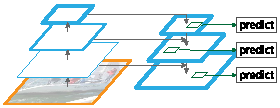
\includegraphics[width=0.7\linewidth]{images/fpn.pdf}
    \caption{Architecture of a feature pyramid network combining features at different scales. Thicker blue outlines indicate semantically stronger features.~\cite{Lin2017}}
    \label{fig:fpn}
\end{figure}

The feature pyramid is built from feature maps at different spatial resolutions produced by different stages of the backbone. The first pyramid layer is the final feature map of the backbone, and each subsequent layer of the pyramid is created by upsampling the previous layer and concatenating it along the channel dimensions with features from an earlier, shallower stage of the backbone. Detections are made independently at each level using several convolutions and the $1 \times 1$ convolutional output layer. The feature pyramid ensures strong semantic information at all levels by combining more meaningful information in upsampled features from deeper layers with fine-grained details from shallower layers.~\cite{Redmon2017, Redmon2018}

\subsection{Ultralytics YOLO}
YOLO has undergone numerous incremental upgrades, incorporating a variety of different deep learning techniques. The Ultralytics implementation of YOLO has become particularly important due to its widespread adoption and active maintenance. It supports multiple computer vision tasks beyond object detection within a single framework, providing interfaces for training, evaluation, and deployment.

Ultralytics also introduced several incremental updates to the architecture, each improving detection performance while maintaining the one-stage architecture and fast inference. \textbf{YOLOv5}~\cite{Jocher2020} introduced several key changes, the most significant addition was the SPPF module, which captures multi-scale context. Other changes included a stem convolution in the backbone, a PANet-style neck for feature fusion, an anchor-based detection head with batch normalization and SiLU activations, and a composite loss for localization, objectness, and classification.

In \textbf{YOLOv8}~\cite{Jocher2023}, the detection head became anchor-free and decoupled, separating classification and regression predictions to improve prediction accuracy. The backbone and neck were adjusted for better multi-scale feature propagation, while retaining SPPF, PANet, and the existing loss function with minor updates. The state-of-the-art version, \textbf{YOLO11}~\cite{Jocher2024}, further optimizes the backbone and neck for small-object detection and multi-scale representation. Its detection head continues to use decoupled regression and classification branches, while SPPF and PANet are retained. The loss function was refined to better balance localization, objectness, and classification.



\chapter{Related Work}
Traditional histopathology relies on optical or electron microscopy to examine tissue samples in order to identify pathological changes and establish diagnoses. In contrast, digital histopathology employs computer methods to visualize histology slides and has become essential in modern clinical practice as it improves diagnostic accuracy and reduces evaluation time. It also enables the use of computer vision and deep learning methods for computer-aided analysis that can automate the process and analyze images with greater consistency and precision than manual examination.

Histological images are typically acquired through whole-slide imaging, which digitizes tissue samples by high-resolution scanning. The images are stored in a pyramidal structure of multiple scans at different resolutions and can contain up to 10 gigapixels, which is too large to be fully examined by human specialists. Deep learning methods are capable of analyzing the full extent of Whole-Slide Images (WSIs), typically by dividing them into smaller patches that are processed individually for feature extraction and classification.

Computer-aided analysis can extract and quantify features in greater detail and perform tasks that would exceed manual capacity. Automated approaches have been successfully applied to identify specific staining, perform tumor staging, detect mitoses, and assess vascular invasion. They are most effective when combined with the expertise of specialist physicians. Automated methods first identify and characterize regions of interest, individual cells, or structures, and classify them based on relevant features. Physicians subsequently interpret and evaluate the obtained results to reach a final diagnosis.~\cite{Moscalu2023}

\paragraph{Nucleus detection} Yousefi and Nie~\cite{Yousefi2019} addressed the problem of nucleus detection in histopathological images, a core task in computational pathology that involves the identification and localization of individual cells. They proposed an efficient pipeline for nucleus classification that can be used for computer-aided ground truth annotation, aiming to reduce the burden of manual labeling and to handle variability in image stain types and resolutions. They leveraged features learned by an object detection model trained on a small annotated dataset to support subsequent classification.

Their method first detects nuclei in histopathological images using a class-agnostic Faster R-CNN~\cite{Ren2015} trained on small annotated patches. For each detected nucleus, feature representations are extracted from multiple levels of the network and used to cluster nuclei into homogeneous subsets using agglomerative hierarchical clustering. Each cluster can then be assigned a single label, allowing all nuclei within the cluster to be annotated in bulk and substantially reducing the total number of manual annotations required. The clustered detections are shown in Figure~\ref{fig:nuclei_det}.

The proposed pipeline generalizes well to unseen nuclei and stain types, as the learned features are used for clustering rather than direct classification. It allows accurate nucleus detection and effective clustering of nuclei for labeling, demonstrating that features learned for object detection in histopathological images can be transferred to nucleus classification in a semi-supervised manner.

\begin{figure}
    \centering
    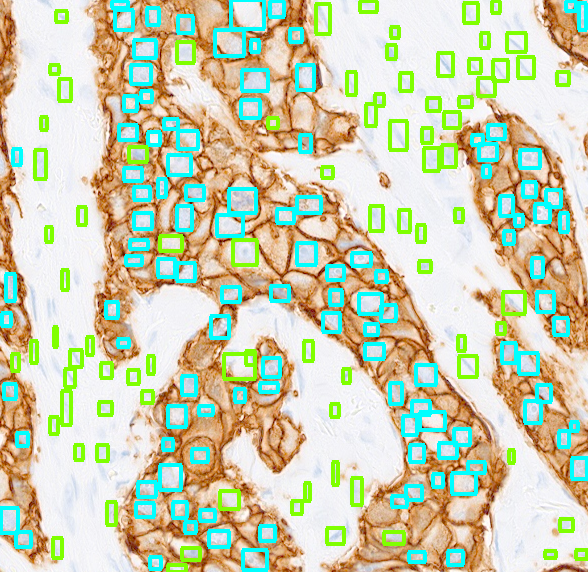
\includegraphics[width=0.5\linewidth]{images/nuclei_detections.png}
    \caption{Class-agnostic Faster R-CNN detections of nuclei in a histological image, clustered based on features extracted from the network.~\cite{Yousefi2019}}
    \label{fig:nuclei_det}
\end{figure}

\paragraph{Mitosis detection in breast cancer} Samonte et al.~\cite{Samonte2023} developed an automated method for detecting mitotic cells in breast cancer histopathological images using YOLOv5~\cite{Jocher2020}. Accurate mitosis detection is critical for evaluating tumor aggressiveness and guiding clinical decisions. Manual counting of mitotic figures is time-consuming, requires specialized pathologists, and is prone to subjectivity and fatigue, motivating the need for an accurate automated approach robust to variability in staining and imaging conditions across different scanners.

Their method divides large pathology images into smaller patches, facilitating processing and focusing on individual cell targets. To increase the diversity of training data and improve model robustness, various data augmentation strategies were applied. Additionally, CycleGAN~\cite{Zhu2017} was employed for color correction to reduce variability caused by different staining protocols and scanners. Detection was performed on the preprocessed and augmented patches using YOLOv5, which incorporates hierarchical feature extraction and multi-scale detection to capture small mitotic targets. The model outputs bounding boxes identifying mitotic cells among many non-mitotic objects.

Evaluation demonstrated that the pipeline achieved higher mean average precision on both internal and external test sets when using preprocessed images compared to uncorrected images. In particular, applying CycleGAN-based color correction improved performance on external test sets, increasing generalization across different scanners and mitigating the decrease in detection accuracy caused by staining variability.

\paragraph{MONKEY Challenge} Automated detection of inflammatory cells in kidney transplant biopsies is the focus of this thesis and will be described in detail in the following chapter. This task was also the objective of the MONKEY Challenge~\cite{Studer2024}, which introduced a dataset of histopathological WSIs with annotations that further divide inflammatory cells between lymphocytes and monocytes.

Deotale et al.~\cite{Deotale2025} approached this problem using an ensemble of two object detection models: the Detection Transformer (DETR)~\cite{Carion2020} with Swin backbone~\cite{Liu2021} and YOLOv5. Their approach is illustrated in Figure~\ref{fig:aira}. Each model was trained separately on two distinct splits of the training data, and their predictions were combined using the weighted box fusion method~\cite{Solovyev2021}, which merges overlapping bounding boxes based on the confidence scores of individual predictions. Based on their evaluation results, DETR was employed for lymphocyte detection, while YOLOv5 was used for monocyte detection. This ensemble strategy demonstrated the complementary strengths of transformer-based and convolutional architectures in improving detection performance in digital pathology.

\begin{figure}[b]
    \centering
    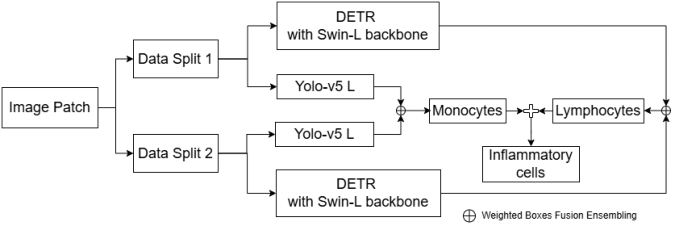
\includegraphics[width=0.95\linewidth]{images/aira_matrix.pdf}
    \caption{Ensemble approach for the detection of inflammatory cells in kidney transplant biopsies, combining DETR detections of lymphocytes and YOLOv5 detections of monocytes.~\cite{Deotale2025}}
    \label{fig:aira}
\end{figure}

Lv et al.~\cite{Lv2025} proposed a multi-headed deep learning architecture KongNet, which is shown in Figure~\ref{fig:kongnet}, for the problem of inflammatory cell detection. The network uses a shared EfficientNetV2~\cite{Tan2021} encoder to extract hierarchical features from input images, followed by multiple parallel decoders, each specialized for a specific cell type. These parallel decoders reduce interference between individual classes by enabling explicit class separation. Spatial and channel squeeze-and-excitation attention modules~\cite{Roy2018} are integrated throughout the network to improve feature representation. These modules emphasize informative regions and suppress irrelevant background, allowing the decoders to capture subtle morphological differences among visually similar cells.

The network is trained end-to-end with a composite multi-task loss that combines detection and segmentation objectives. Each decoder simultaneously predicts cell centroids, segmentation masks, and contours, allowing the network to learn discriminative morphological features for its target class. This multi-task learning setup encourages the use of auxiliary predictions of nuclei and contour masks to promote the learning of fine-grained morphological representations, supporting robust differentiation between closely related cell types.

KongNet demonstrated strong performance in nuclei detection and classification across various tissue and staining types and achieved first place in one of the MONKEY Challenge tracks. The results indicate that combining class-specific decoders with attention modules and auxiliary tasks improves localization and classification of closely related cell types, supporting accurate and generalizable performance in complex histopathological images.

\begin{figure}
    \centering
    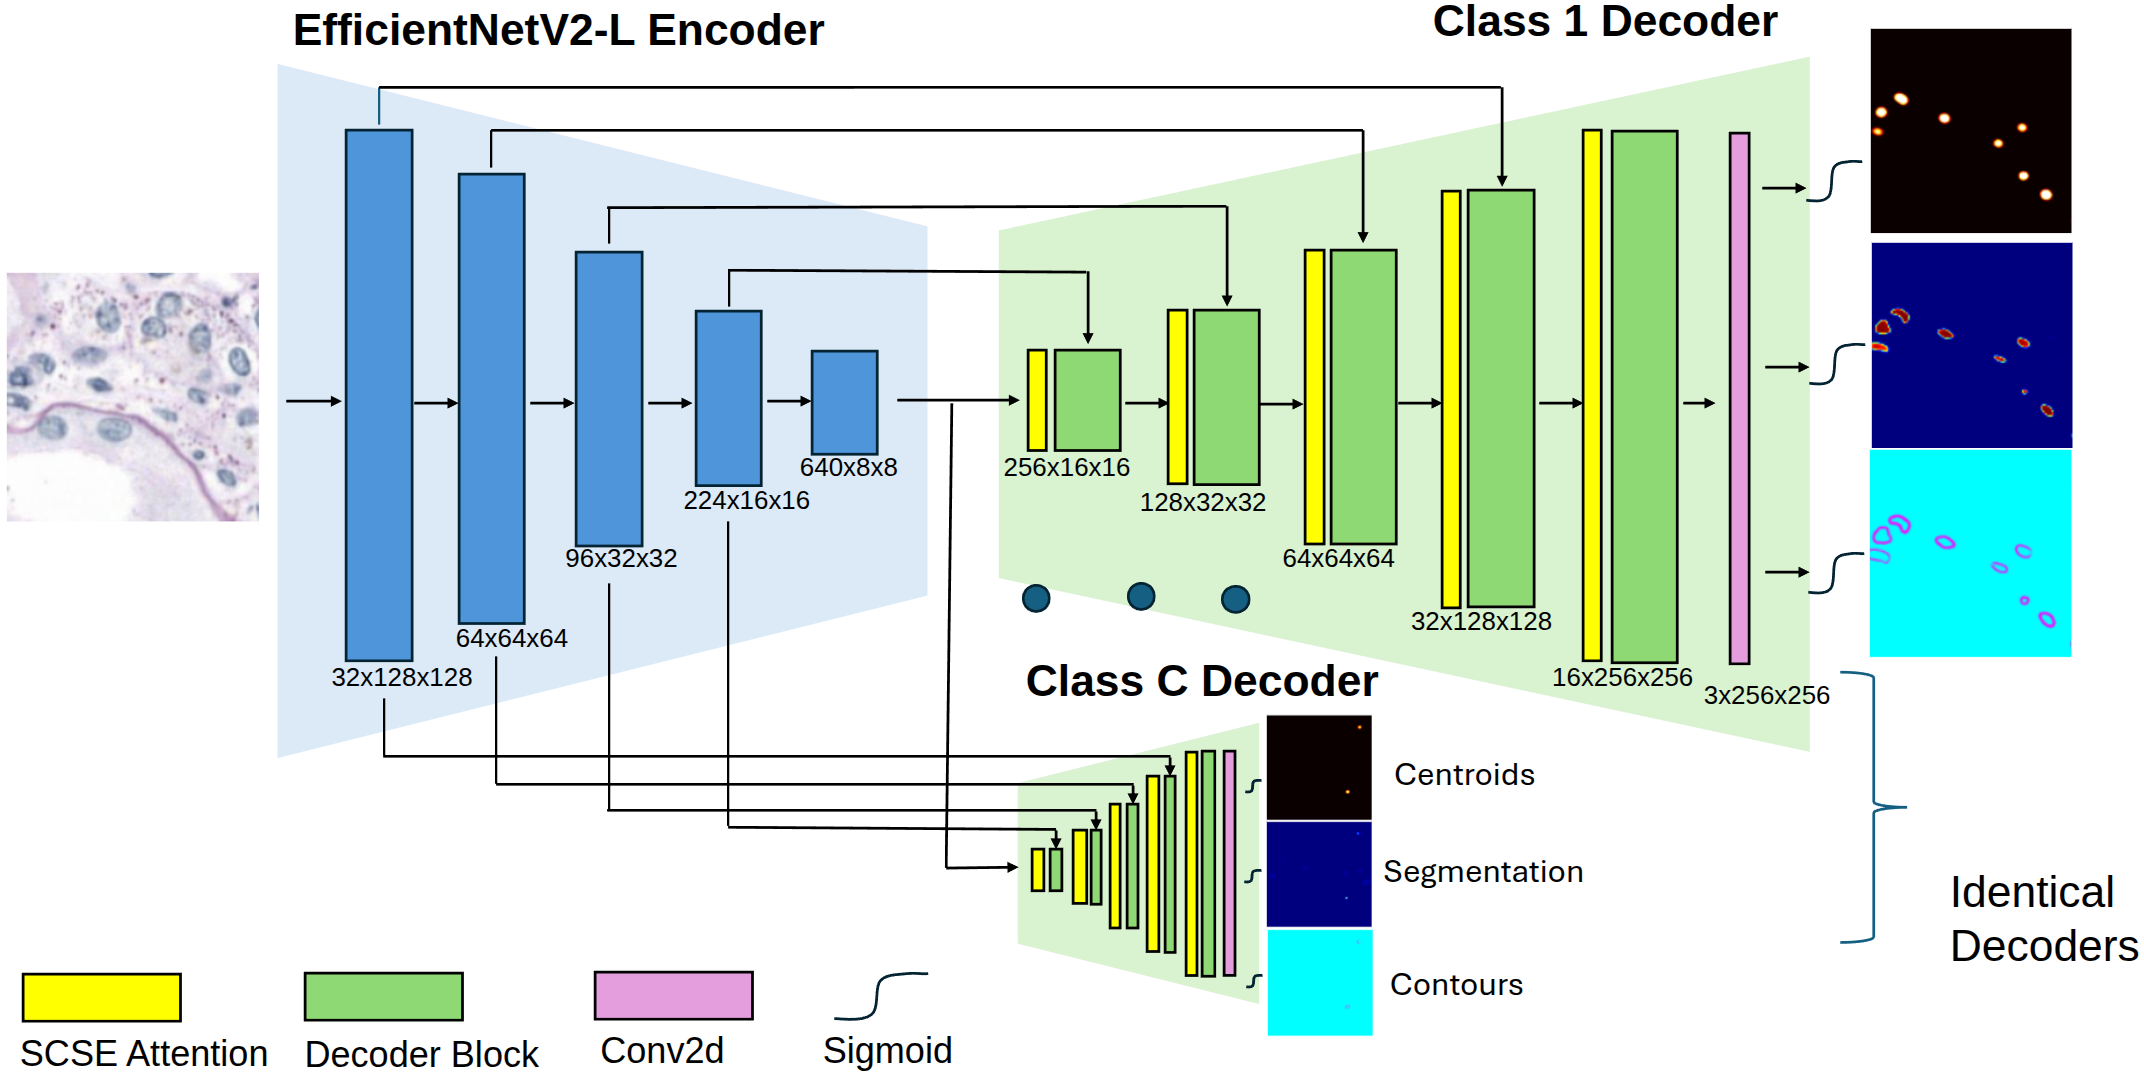
\includegraphics[width=\linewidth]{images/kongnet.png}
    \caption{KongNet architecture consisting of a shared encoder and multiple specialized decoders, each predicting cell centroids, segmentation masks, and contours.~\cite{Lv2025}}
    \label{fig:kongnet}
\end{figure}



\chapter{Proposed Approach for Detecting Inflammatory Cells in Kidney Transplant Biopsies}
This chapter presents a deep learning approach for the automated assessment of kidney transplant biopsies. These biopsies are performed to evaluate the condition of the transplanted organ and guide treatment aimed at preventing transplant failure. A key component of biopsy assessment is the identification and quantification of \textbf{mononuclear inflammatory cells}, which play an essential role in transplant rejection. Automating their detection could reduce the workload of pathologists while improving the consistency and efficiency of the overall assessment.

In this work, I developed a deep learning model for the detection of mononuclear inflammatory cells in kidney transplant biopsies and their subsequent classification into \textbf{lymphocytes} and \textbf{monocytes}. Although this subdivision is not performed in practice, it is hypothesized that it could provide additional information relevant to disease progression. The model was trained using a histological dataset with dot annotations of inflammatory cells provided by the MONKEY Challenge~\cite{Studer2024}. The data originate from routine diagnostics conducted in different pathology departments, and their preparation involves cutting the biopsies into thin tissue sections, fixing them onto glass slides, staining them, and digitizing them using a WSI scanner.

Given the form of the provided annotations, I decided to frame the problem as an object detection task rather than image segmentation, which is commonly used in digital histopathology to localize and delineate individual cells. In this application, precise cell delineation is not required, and the dataset does not provide ground truth segmentation masks, making segmentation unnecessarily complex. An overview of the proposed approach is shown in Figure~\ref{fig:diagram}. High-resolution WSIs were first divided into patches of fixed size, and the provided dot annotations were converted into bounding box labels suitable for object detection training. The object detection CNN YOLO11~\cite{Jocher2024} was then trained using these labels, and its performance was evaluated under various hyperparameter settings. Several experiments were conducted to improve its performance, focusing mainly on generating higher-quality training labels, as data quality is critical for effective model learning. Finally, the proposed approach was compared with other solutions submitted to the MONKEY Challenge.

\begin{figure}
    \centering
    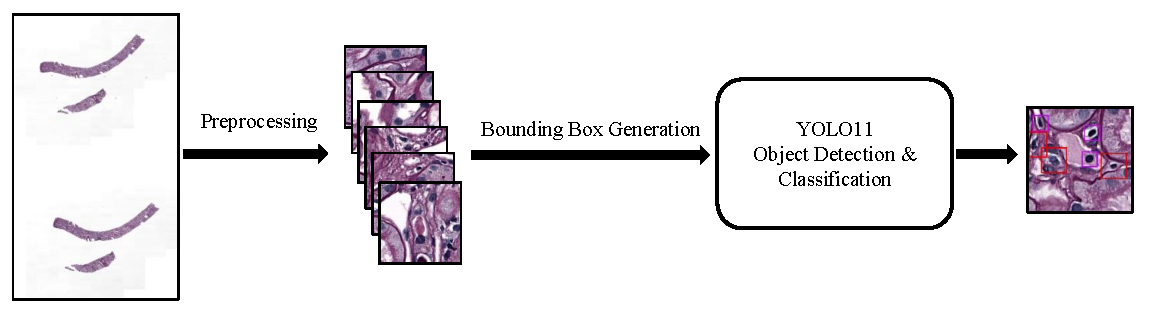
\includegraphics[width=\linewidth]{images/diagram.pdf}
    \caption{Diagram of the approach used to develop a deep learning model for the detection of lymphocytes and monocytes in kidney transplant biopsies.}
    \label{fig:diagram}
\end{figure}


\section{Dataset}
The provided training dataset consists of 81 WSIs of kidney transplant biopsies from four different pathology departments. On average, each WSI covers 512 $\mathrm{mm^2}$ at a resolution of 0.24 \textmu m/pixel, roughly corresponding to dimensions of $67\,000 \times 127\,000$ pixels. The WSIs are too large to be fully annotated, so mononuclear inflammatory cells are labeled only within selected polygonal Regions of Interest (ROIs), with each WSI containing at least one ROI. The training dataset contains 164 ROIs with an average area of 0.31 $\mathrm{mm^2}$, or roughly $2\,700 \times 2\,400$ pixels. Introduction Figure~\ref{fig:monkey} shows a sample WSI and ROI with annotations. On average, there are 360 lymphocytes and 190 monocytes in each ROI, which is approximately a 2:1 ratio.

Each training sample consists of two WSI scans with different stains: Periodic Acid-Schiff (PAS), the standard staining for the kidney, and Immunohistochemistry (IHC), which can be used to differentiate lymphocytes from monocytes. The two stains, shown in Figure~\ref{fig:stain}, are co-registered, ensuring that they share a common coordinate system. Only PAS staining is meant to be used for inference, as it is the primary staining used by pathologists when assessing kidney biopsies, while IHC staining was used to guide the annotation process and may be utilized during model training. IHC employs cell-specific markers, producing dark brown cytoplasmic staining of lymphocytes and nuclear magenta staining of monocytes. The MONKEY Challenge also provides hold-out validation and test sets from two additional pathology centers, consisting of 9 and 26 PAS-stained WSIs, respectively.

\begin{figure}
    \centering
    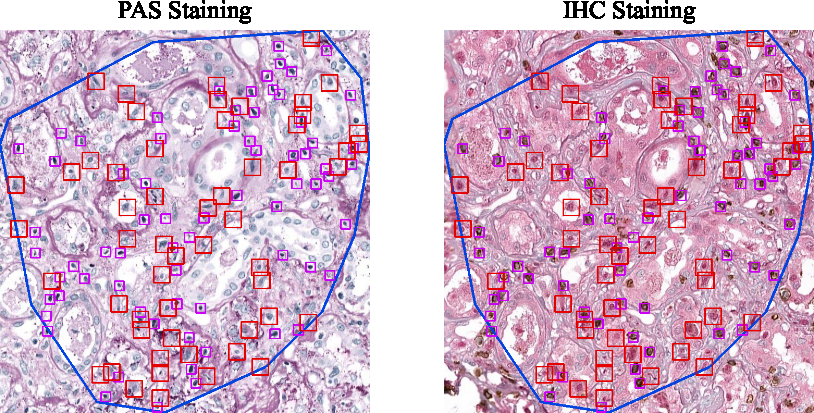
\includegraphics[width=\linewidth]{images/staining.pdf}
    \caption{PAS and IHC staining of the same ROI marked by a blue polygon. Bounding boxes are drawn around provided dot annotations for lymphocytes (purple) and monocytes (red).}
    \label{fig:stain}
\end{figure}

\subsection{Preprocessing}
WSIs cannot be used directly for model training due to their size and the absence of annotations outside ROIs. ROIs are fully annotated, but still too large to be processed by object detection models in a single forward pass. Therefore, I divided each ROI into a set of fixed-size square patches suitable for batch processing during model training and inference. A regular grid was overlaid over each ROI and patches entirely contained within the ROI were accepted into the processed dataset. Patches overlapping the ROI boundary were rejected to avoid the inclusion of any unannotated inflammatory cells, which could mislead the model during training.

To maximize ROI coverage, the grid was aligned with its topmost and leftmost points and shifted along the x and y axes in three increments, each equal to a quarter of the chosen patch size. This produced 16 possible grid positions, and the position accepting the most patches was selected. The inflammatory cell annotations were then divided among the created patches and, since the annotations are only points, each was assigned to a single patch. Cells located in patches overlapping ROI boundaries were omitted from the dataset along with the patches. The resulting dataset was split into training and validation sets in a 4:1 ratio.

I created three separate datasets with patch side lengths of 512, 256, and 128 pixels. The complete WSI dataset contains $90\,367$ cells. As patch size increases, more cells are omitted due to reduced granularity of the overlaid grid, as shown in Table~\ref{tab:patches}. To retain more data, it would be better to use smaller patch sizes for training. In contrast, larger patches contain more contextual information, more cells per patch, and reduce the total number of patches, allowing faster training. Unless stated otherwise, all figures in this chapter depict patches with side lengths of 256 pixels.

\begin{table}
    \centering
    \begin{tabular}{r|rrrr}
        \toprule
        Patch Size & \#Patches & \#Cells & \#Cells Omitted & Avg Cells/Patch \\
        \midrule
        512 & $2\,162$ & $56\,752$ & $33\,615$ & 26.2\\
        256 & $10\,756$ & $72\,665$ & $17\,702$ & 6.8\\
        128 & $47\,931$ & $81\,717$ & $8\,650$ & 1.7\\
        \bottomrule
    \end{tabular}
    \caption{Dataset size and cell counts after preprocessing with different patch sizes.}
    \label{tab:patches}
\end{table}


\section{Bounding Box Generation}
The provided annotations mark each mononuclear inflammatory cell with a single point, whereas object detection models learn from and predict bounding boxes. The annotations therefore need to be converted into bounding box labels that are centered on the respective cells and accurately capture their extent. However, the dot annotations provide no information about cell dimensions and only mark their approximate centers. The simplest approach is to create a fixed-size bounding box around each annotation based on the average diameter of the corresponding cell type. This ensures that the bounding boxes are centered on the annotated spot, but their dimensions may not accurately reflect the true size of the inflammatory cells.

The bounding box dimensions can be refined using a segmentation model. For this purpose, I used \textbf{Segment Anything Model 2 (SAM 2)}~\cite{Ravi2024}, a transformer-based model for zero-shot, promptable segmentation in images and videos that can adapt to new domains with zero prior knowledge. Given an input prompt, such as a point or a bounding box referring to an object of interest in the image, SAM 2 outputs a valid segmentation mask. SAM 2 has been used in a wide range of applications, including medical image segmentation. The provided dot annotations can serve as prompts for SAM 2 to predict the segmentation masks of inflammatory cells. Based on these considerations, I defined three types of bounding box labels:
\begin{description}
    \item[BasicBox] Square bounding boxes of fixed size around each dot annotation, based on the average diameters of lymphocytes and monocytes. Reported cell diameters vary between sources, typically in the range of 6--10 \textmu m for lymphocytes~\cite{Studer2024, Mathur2013} and 12--22 \textmu m for monocytes~\cite{Studer2024, Tigner2025, Espinoza2025}. I selected bounding box side lengths of 9 \textmu m for lymphocytes and 15 \textmu m for monocytes, corresponding to 37 and 62 pixels, respectively, visually based on the training data. BasicBoxes that overlapped the patch boundary were clipped to cover only the visible part of the respective cells.

    \item[SegBox] Bounding boxes that tightly enclose segmentation masks predicted by SAM 2 prompted with the provided dot annotations. Predictions were performed using the base version of SAM 2.1 implemented in the Ultralytics Python package. These predictions are not perfectly accurate and require validation to ensure that the derived bounding boxes are reliable. The validation was performed using the average cell diameter as a reference, which is the only available information about the actual cell dimensions.
    
    Therefore, boxes with either width or height exceeding 1.5 times the corresponding BasicBox dimensions were removed from the dataset, leaving the respective cells unlabeled. This postprocessing was applied because unusually large boxes presumably indicate incorrect segmentation predictions. The relatively low threshold was chosen because the predicted SegBoxes are generally much smaller than BasicBoxes, as illustrated in Figure~\ref{fig:boxes}. In the validation split, missing SegBox labels were replaced with BasicBoxes to enable more accurate model performance estimation.
    
    \item[MixedBox] SegBoxes can leave many inflammatory cells unlabeled, which can potentially impair model training. To address this, BasicBoxes and SegBoxes can be combined to retain all labels while incorporating improved estimation of cell dimensions. MixedBox labels were created by replacing SegBoxes that could not be reliably segmented and were filtered out during postprocessing with the corresponding BasicBoxes.
\end{description}

\begin{figure}
    \centering
    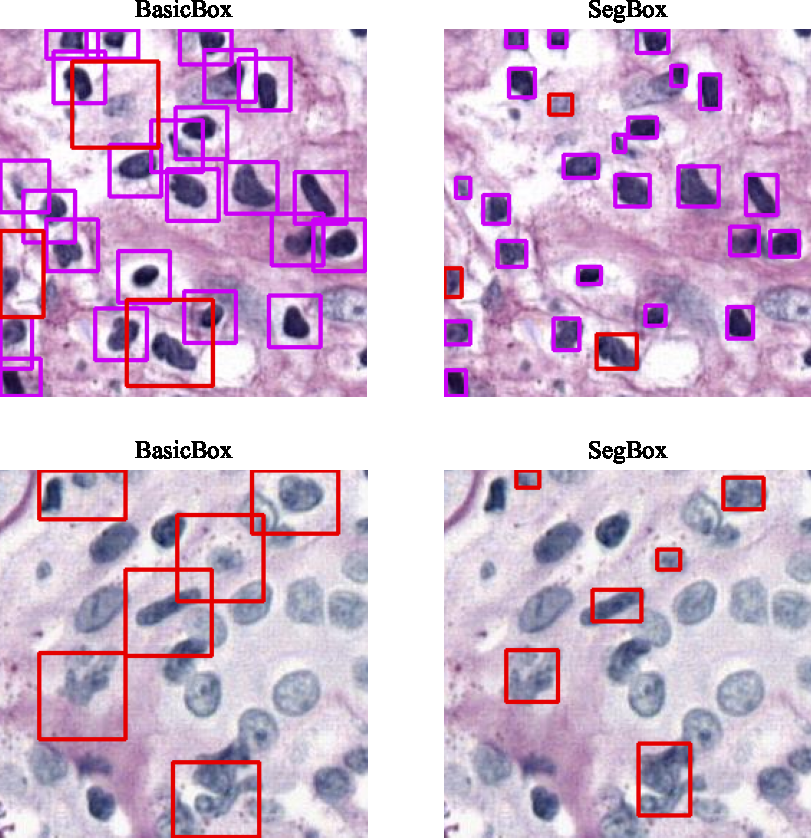
\includegraphics[width=\linewidth]{images/boxes_comparison.pdf}
    \caption{Comparison of different types of bounding box labels for lymphocytes (purple) and monocytes (red). SegBoxes in the top row accurately cover the inflammatory cells, while BasicBoxes often significantly overlap each other or overestimate cell sizes. In contrast, the bottom row shows some SegBoxes merging multiple cells or only partially covering individual cells, with BasicBoxes being more accurate.}
    \label{fig:boxes}
\end{figure}

\paragraph{Box comparison} The differences between the proposed bounding box labels are illustrated in Figure~\ref{fig:boxes}, and the label counts and average bounding box dimensions are reported in Table~\ref{tab:boxes}. BasicBoxes are the most reliable labels, as they are always centered on the corresponding dot annotations and are never missing. Their main limitation is that they can substantially overestimate the size of certain inflammatory cells, especially monocytes. In addition, when cells appear in clusters, their labels often overlap. The average dimensions of BasicBoxes deviate from the predefined fixed values and gradually decrease with smaller patch sizes because the bounding boxes are clipped to patch boundaries, which occurs more frequently in smaller patches.

The main advantage of SegBoxes is that they reflect the real size of each individual cell. However, their quality depends on the accuracy of SAM 2, and there is no guarantee that its predictions are reliable. SegBoxes sometimes fail to cover the full extent of a cell, merge adjacent cells into a single bounding box, and leave many inflammatory cells unlabeled, as shown in Table~\ref{tab:boxes}. These missing labels often result from SAM 2 segmenting the corresponding cells as part of the surrounding background, producing a substantially larger bounding box that is consequently filtered out. The proportion of missing labels decreases with decreasing patch size, from 24.4\% in the largest patches to 6.8\% in the smallest. However, this does not necessarily imply that the predicted segmentation masks are more accurate in smaller patches, as it is also possible that the filtering condition becomes insufficient.

\begin{table}
    \centering
    \begin{tabular}{llrrrr}
        \toprule
        Label Type & Staining & Patch Size & \#Cells & \multicolumn{2}{c}{Avg Box Dimensions} \\
        & & & & Lymphocytes & Monocytes \\
        \midrule
        BasicBox & PAS/IHC & 512 & $56\,752$ & $36.5 \times 36.5$ & $60.2 \times 60.1$ \\
        BasicBox & PAS/IHC & 256 & $72\,665$ & $35.9 \times 35.8$ & $58.2 \times 58.3$ \\
        BasicBox & PAS/IHC & 128 & $81\,717$ & $34.5 \times 34.5$ & $54.4 \times 54.5$ \\
        \midrule
        SegBox & PAS & 512 & $42\,881$ & $17.8 \times 18.5$ & $21.0 \times 21.9$ \\
        SegBox & PAS & 256 & $65\,760$ & $16.7 \times 17.2$ & $18.8 \times 19.6$ \\
        SegBox & PAS & 128 & $76\,186$ & $14.8 \times 15.1$ & $16.1 \times 16.6$ \\
        \midrule
        MixedBox & PAS & 512 & $56\,752$ & $22.0 \times 22.6$ & $31.9 \times 32.7$ \\
        MixedBox & PAS & 256 & $72\,665$ & $18.3 \times 18.9$ & $23.5 \times 24.3$ \\
        MixedBox & PAS & 128 & $81\,717$ & $15.9 \times 16.1$ & $20.0 \times 20.4$ \\
        \midrule
        SegBox & IHC & 512 & $42\,540$ & $29.0 \times 29.6$ & $26.8 \times 27.5$ \\
        SegBox & IHC & 256 & $55\,463$ & $25.9 \times 26.3$ & $23.4 \times 23.8$ \\
        SegBox & IHC & 128 & $57\,704$ & $20.6 \times 21.6$ & $19.5 \times 20.4$ \\
        \bottomrule
    \end{tabular}
    \caption{Average bounding box dimensions in pixels for each label type, together with the total number of retained cells labels.}
    \label{tab:boxes}
\end{table}

SegBoxes generated from IHC-stained patches are on average larger than those from PAS-stained patches, especially for lymphocytes. Interestingly, SAM 2 reliably segments fewer inflammatory cells in IHC-stained patches than in PAS-stained ones, despite IHC staining being generally considered more discriminative. This is most likely caused by suboptimal staining in certain WSIs or subtle spatial shifts between corresponding PAS and IHC WSIs, both of which occasionally occur in the provided dataset. The IHC staining protocol is relatively sophisticated and prone to errors, sometimes leading to weak staining intensity or aspecific background staining. The spatial misalignment between the two WSI stains can cause the dot annotations to be slightly offset from the corresponding cells in the IHC images, thereby preventing successful segmentation.

MixedBoxes address the issue of missing SegBox labels, which could otherwise reduce the performance of models that utilize them for training. Such models might potentially learn to distinguish and avoid predicting the types of cells that SAM 2 fails to segment reliably and that are therefore omitted from the dataset. However, SegBoxes are on average significantly smaller than BasicBoxes, as shown in Table~\ref{tab:boxes}, and combining the two types into MixedBoxes produces a dataset with two substantially different bounding box distributions, which may also negatively affect object detection training.

\paragraph{Padding} The generated SegBoxes can be padded by adding a fixed number of pixels on all sides to enlarge their dimensions and ensure that they fully cover the corresponding inflammatory cells. The effect of padding is illustrated in Figure~\ref{fig:padding} and summarized in Table~\ref{tab:padding}. SegBoxes padded with ten pixels are visually and on average very similar in size to BasicBoxes. The average dimensions of lymphocyte labels are nearly identical, and although this similarity is less pronounced for monocytes, their dimensions also become considerably closer.

In contrast to regular SegBoxes, which tightly enclose each inflammatory cell, SegBoxes with ten pixels of padding can be used to only adjust the position of misaligned BasicBoxes caused by imprecise dot annotations. They still reduce the dimensions of excessively large boxes and thus preserve more accurate cell size estimation. Padding can also be applied to MixedBoxes by padding only the included SegBoxes. This results in a dataset with more consistent bounding box sizes across all cells, as shown in Table~\ref{tab:padding}, compared to unpadded MixedBoxes.

\begin{table}
    \centering
    \begin{tabular}{llrrr}
        \toprule
        Label Type & Padding & \multicolumn{2}{c}{Avg Box Dimensions} \\
        & & Lymphocytes & Monocytes \\
        \midrule
        BasicBox & -- & $36.5 \times 36.5$ & $60.2 \times 60.1$ \\
        \midrule
        SegBox & 5 & $27.5 \times 28.2$ & $30.7 \times 31.6$ \\
        SegBox & 10 & $37.2 \times 37.8$ & $40.2 \times 41.1$ \\
        \midrule
        MixedBox & 5 & $29.6 \times 30.2$ & $39.0 \times 39.7$ \\
        MixedBox & 10 & $37.0 \times 37.6$ & $45.9 \times 46.6$ \\
        \bottomrule
    \end{tabular}
    \caption{Average bounding box dimensions of pixels after adding five or ten pixels of padding on all sides to SegBox and MixedBox labels in patches of size 512.}
    \label{tab:padding}
\end{table}

\begin{figure}
    \centering
    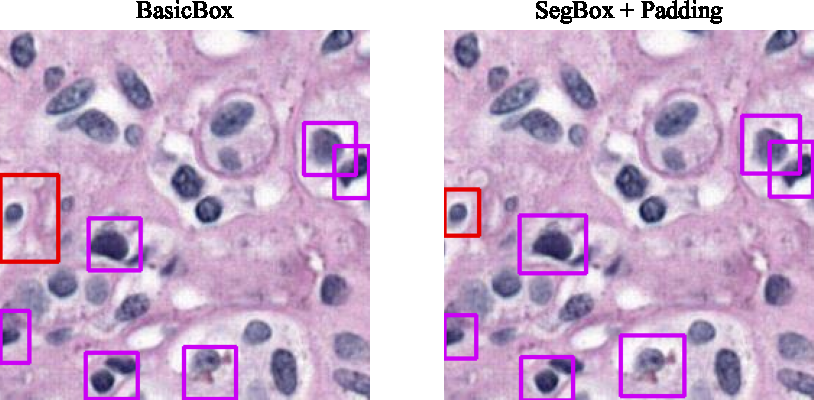
\includegraphics[width=\linewidth]{images/padding.pdf}
    \caption{Visual comparison of BasicBox labels and SegBox labels padded by ten pixels on all sides for lymphocytes (purple) and monocytes (red).}
    \label{fig:padding}
\end{figure}


\section{Model Training and Validation}
The preprocessed kidney transplant biopsy dataset and the proposed bounding box labels can be used to train an object detection model. I decided to use the one-stage convolutional object detection network \textbf{YOLO11}~\cite{Jocher2024} and its implementation from the Ultralytics Python package. YOLO11 was selected because it is the state-of-the-art YOLO model, combining excellent performance on various benchmarks with fast inference and training compared to other object detection models. I utilized YOLO11 pre-trained on the COCO dataset~\cite{Lin2014} and fine-tuned it on the training split of the preprocessed dataset, which consists of a randomly selected 80\% of the total patches. 

During fine-tuning, the Ultralytics implementation heuristically selected an optimizer and an initial learning rate based on the size of the training dataset. \textbf{AdamW}~\cite{Loshchilov2019} with an initial learning rate value of 0.0017 was selected for patch size 512, while \textbf{SGD} with an initial learning rate of 0.01 was selected for patch sizes 256 and 128. The model was trained with batch size 16, momentum factor 0.9, weight decay term 0.0005, and input image size equal to the patch size of the training dataset.

Automatic mixed precision~\cite{Micikevicius2018} was enabled to reduce memory usage and accelerate training. A \textbf{cosine learning rate scheduler} was utilized to gradually reduce the learning rate to a final value equal to 0.01 times the initial learning rate following a cosine curve. Early stopping was disabled to ensure that the scheduler reached the final learning rate for better convergence, and the total number of epochs was tuned when selecting the baseline model. Three initial warm-up epochs were used to stabilize early training.

\textbf{Data augmentation} was applied during training, mostly using the default settings from the Ultralytics implementation. Augmentations were applied online, with their values selected for each image randomly from a predefined range. They included image translation, rotation, horizontal and vertical flipping, and hue, saturation, and brightness jitter. I reduced the saturation jitter ratio from 0.7 to 0.4 to match the brightness jitter ratio and enabled image rotation and vertical flipping, as inflammatory cells can appear in any orientation. I also disabled image scaling and mosaic augmentation~\cite{Bochkovskiy2020}, which is a generalization of cutmix~\cite{Yun2019} to four images, because cell size and the surrounding context are presumably important predictors, and varying them could harm the training.

During validation and inference, the model used the same input size as during training. \textbf{Class-agnostic NMS} was applied with the default IoU threshold of 0.7 to remove overlapping predictions regardless of class. I decided to use class-agnostic NMS because the model can and sometimes does predict a bounding box for both a lymphocyte and a monocyte around the same cell. Standard NMS, which is applied independently for each class, would fail to recognize these predictions as duplicates, whereas class-agnostic NMS keeps only the higher-confidence prediction even if their classes are different.

\subsection{Model Evaluation}
The model performance was evaluated on the validation split of the preprocessed dataset, which consists of the remaining 20\% of patches. I used AP as the primary performance metric, defined in Equation~\ref{eq:ap} and calculated after matching the predictions with ground truth labels within each patch using Algorithm~\ref{alg:matching}. AP is calculated per class, with the mAP being its average across both classes that represents overall performance. I selected this metric because it is standard in object detection benchmarks~\cite{Everingham2010, Lin2014} and effectively captures the precision-recall trade-off across different confidence thresholds. I used AP with an IoU threshold of 0.5 rather than stricter variants such as $\mathrm{AP}_{50:95}$ because the assessment of kidney transplant biopsies prioritizes high precision and recall over perfect cell localization.

Calculating AP with an IoU threshold relative to bounding box labels evaluates how well the model has learned to predict the boxes. However, the bounding boxes were generated from dot annotations and are not guaranteed to be accurate. For example, if the training boxes better represent the inflammatory cells but are harder for the model to learn, this \textbf{box-wise AP} may decrease even if the actual cell predictions improve and vice versa. Therefore, the quality of the bounding boxes must be considered before interpreting the box-wise AP.

The entire training pipeline, including dataset preprocessing, bounding box generation, and object detection, can be evaluated in a single step by calculating AP directly relative to the provided dot annotations. The resulting \textbf{point-wise AP} is independent of the specific type of bounding box labels, making it better comparable across different experiments. Point-wise AP is calculated identically to box-wise AP, with only the IoU threshold replaced by a simple distance threshold between the center of the predicted bounding box and the ground truth dot annotation. Following the MONKEY Challenge evaluation, this distance threshold is set to 4 \textmu m for lymphocytes and 5 \textmu m for monocytes.

The exact AP calculation and algorithm for matching predictions with ground truth labels are not standardized and the Ultralytics implementation, which was used to calculate box-wise AP, differs slightly from the definition in Equation~\ref{eq:ap} and Algorithm~\ref{alg:matching}. It greedily matches predictions to ground truth labels based only on their IoU instead of taking prediction confidence into consideration. It also does not interpolate the precision-recall curve, and calculates AP directly as the area under the curve using the trapezoidal rule. For consistency, I implemented the point-wise AP using the same approach as Ultralytics so the two metrics are better comparable. These differences have no significant effect on the final AP values and do not compromise performance comparisons when the calculation is applied consistently.


\section{Baseline Model}
With the training and validation setup and performance metrics defined, the baseline YOLO11 model was selected. The size of the baseline model, the patch size of the training dataset, and the number of training epochs were chosen based on performance comparison on PAS-stained patches with BasicBox labels. All training for this comparison was performed on GPUs available from ClusterFIT.

The model size was selected by training the YOLO11 S, M, L, and X versions for 200 epochs on patch size 512. The results in Table~\ref{tab:yolo_size} show that larger models perform slightly better. The reported training times are not fully comparable because the models were trained on different GPUs that were assigned according to their availability. Validation losses and performance metrics for all model sizes plateaued around 100 epochs and then slightly decreased for the smaller models. I selected YOLO11 M as the baseline to balance performance with training time, as performance gains from larger models were relatively small.

\begin{table}[h]
    \centering
    \begin{tabular}{cr|rrrrrrr}
        \toprule
        Model & Params & \multicolumn{3}{c}{Box-wise AP} & \multicolumn{3}{c}{Point-wise AP} & Time \\
        & & L & M & \textbf{mAP} & L & M & \textbf{mAP} & \\
        \midrule
        S & 9.4 M & 0.738 & 0.472 & 0.605 & 0.665 & 0.372 & 0.519 & 1.3 h \\
        M & 20.1 M & 0.742 & 0.473 & 0.607 & 0.662 & 0.377 & 0.520 & 1.5 h \\
        L & 25.3 M & 0.755 & 0.493 & 0.624 & 0.662 & 0.402 & 0.532 & 2.3 h \\
        X & 56.9 M & 0.764 & 0.497 & \textbf{0.630} & 0.697 & 0.409 & \textbf{0.553} & 1.9 h \\
        \bottomrule
    \end{tabular}
    \caption{Performance of different YOLO11 sizes trained on patch size 512 for 200 epochs. Training times are not fully comparable because the models were trained on different GPUs. L: lymphocytes, M: monocytes, mAP: mean average precision.}
    \label{tab:yolo_size}
\end{table}

YOLO11 M was then trained on different patch sizes for varying numbers of epochs. The results in Table~\ref{tab:epochs} show that the model performs slightly better on larger patch sizes. The reported training times are again not fully comparable but clearly indicate that training is significantly faster on datasets with larger patch sizes because they contain fewer patches overall. Validation loss curves and performance metrics for models trained on patch sizes 512 and 256 plateaued after about 100 epochs, while models trained on patch size 128 plateaued after approximately 200 epochs. All models showed slight overfitting after saturation, with the models trained on patch size 512 overfitting the most.

The model was also evaluated with the default data augmentation settings, trained for 200 epochs on different patch sizes. The default settings include image scaling, mosaic augmentation, higher saturation jitter, and disable image rotation and vertical flipping. Performance was nearly identical, but validation loss curves fluctuated significantly more and all models reached saturation only after 200 epochs, indicating that training was more unstable and slower. Test-time augmentation was also tested, but did not bring any benefits and slightly decreased performance.

Based on these results, I selected YOLO11 M trained on patch size 512 for 100 epochs as the baseline model. All models consistently performed significantly better in lymphocyte detection than in monocyte detection. This could be caused because there are approximately twice as many lymphocytes in the training dataset, or because BasicBox labels fit lymphocytes better, or perhaps because monocyte detection is inherently a harder task. Box-wise AP was consistently higher than point-wise AP across all experiments, indicating that IoU with BasicBoxes is a more lenient threshold than the point-wise distance threshold.

\begin{table}
    \centering
    \begin{tabular}{rr|rrrrrrr}
        \toprule
        Patch & Epochs & \multicolumn{3}{c}{Box-wise AP} & \multicolumn{3}{c}{Point-wise AP} & Time \\
        & & L & M & \textbf{mAP} & L & M & \textbf{mAP} & \\
        \midrule
        512 & 100 & 0.785 & 0.525 & \textbf{0.655} & 0.707 & 0.418 & \textbf{0.562} & 1.0 h \\
        512 & 200 & 0.742 & 0.473 & 0.607 & 0.662 & 0.377 & 0.520 & 1.5 h \\
        512 & 300 & 0.695 & 0.428 & 0.561 & 0.616 & 0.325 & 0.471 & 5.7 h \\
        \midrule
        256 & 100 & 0.769 & 0.489 & \textbf{0.629} & 0.667 & 0.355 & \textbf{0.511} & 2.8 h \\
        256 & 200 & 0.766 & 0.487 & 0.626 & 0.663 & 0.359 & \textbf{0.511} & 7.0 h \\
        256 & 300 & 0.743 & 0.467 & 0.605 & 0.660 & 0.347 & 0.504 & 9.8 h \\
        \midrule
        128 & 100 & 0.746 & 0.474 & 0.610 & 0.666 & 0.361 & 0.513 & 8.2 h \\
        128 & 200 & 0.752 & 0.489 & \textbf{0.620} & 0.657 & 0.373 & \textbf{0.515} & 18.1 h \\
        128 & 300 & 0.739 & 0.460 & 0.599 & 0.638 & 0.358 & 0.498 & 37.2 h \\
        \bottomrule
    \end{tabular}
    \caption{Performance of YOLO11 M trained on different patch sizes for different numbers of epochs. L: lymphocytes, M: monocytes, mAP: mean average precision.}
    \label{tab:epochs}
\end{table}


\section{Experiments}
The following experiments aimed to improve the baseline performance, primarily by enhancing the quality of the generated bounding boxes, since the quality of the training dataset is crucial for model performance. Baseline evaluation showed that YOLO11 performs best when trained on patches of size 512, although the margin was relatively small. Larger patches are likely favorable because they contain more context around each cell and fewer cells truncated at patch boundaries and only partially visible within individual patches. However, smaller patches contain significantly more cells overall, as shown in Table~\ref{tab:patches}, and a larger training dataset typically leads to better performance.

Therefore, all experiments were conducted using all patch sizes to ensure proper evaluation. YOLO11 M was trained on GPUs available from ClusterFIT for 200 epochs in each experiment to avoid possible underfitting. When overfitting was observed in validation loss curves and performance metrics, the model was retrained for 100 epochs instead. This approach was chosen instead of early stopping to ensure that the cosine learning rate scheduler completed its full schedule. For each model in a given experiment, results are reported for the training run that achieved the best performance. Whenever the performance of a specific patch size or bounding box type is mentioned in this section, it refers to the performance of YOLO11 trained under that setting.

\subsection{Bounding Box Types}
The first experiment evaluated the performance of models trained with different types of bounding box labels. Table~\ref{tab:exp_labels} shows that the differences between patch sizes are more pronounced for SegBoxes than in the previous comparison, with patch size 256 performing best. Most notably, the SegBox box-wise AP is substantially lower than the baseline, whereas the decrease in point-wise AP is less pronounced.

The different behavior of the two metrics is most likely due to the significantly smaller average dimensions of SegBoxes compared to BasicBoxes, as shown in Table~\ref{tab:boxes}. For smaller bounding boxes, the same absolute pixels shift results in a larger decrease in IoU, making the IoU threshold more sensitive to localization errors and relatively stricter. In contrast, the point-wise threshold remains unaffected by the box size. Consequently, SegBox point-wise AP is generally higher than the corresponding box-wise AP, unlike the relationship observed for BasicBoxes.

\begin{table}[h]
    \centering
    \begin{tabular}{lr|rrrrrr}
        \toprule
        Label Type & Patch & \multicolumn{3}{c}{Box-wise AP} & \multicolumn{3}{c}{Point-wise AP} \\
        & & L & M & \textbf{mAP} & L & M & \textbf{mAP} \\
        \midrule
        BasicBox & 512 & 0.785 & 0.525 & \textbf{0.655} & 0.707 & 0.418 & \textbf{0.562} \\
        BasicBox & 256  & 0.769 & 0.489 & 0.629 & 0.667 & 0.355 & 0.511 \\
        BasicBox & 128  & 0.752 & 0.489 & 0.620 & 0.657 & 0.373 & 0.515 \\
        \midrule
        SegBox & 512 & 0.559 & 0.296 & 0.427 & 0.610 & 0.320 & 0.465 \\
        SegBox & 256 & 0.638 & 0.329 & \textbf{0.483} & 0.652 & 0.312 & \textbf{0.482} \\
        SegBox & 128 & 0.576 & 0.235 & 0.406 & 0.619 & 0.270 & 0.445 \\
        \midrule
        MixedBox & 512 & 0.652 & 0.351 & \textbf{0.502} & 0.477 & 0.217 & 0.347 \\
        MixedBox & 256 & 0.647 & 0.336 & 0.492 & 0.585 & 0.293 & \textbf{0.439} \\
        MixedBox & 128 & 0.597 & 0.249 & 0.423 & 0.537 & 0.208 & 0.373 \\
        \bottomrule
    \end{tabular}
    \caption{Performance of models trained with different types of bounding box labels. L: lymphocytes, M: monocytes, mAP: mean average precision.}
    \label{tab:exp_labels}
\end{table}

Despite this, SegBoxes still perform worse than BasicBoxes even when evaluated using point-wise AP. This decline in performance might be caused by the presence of unlabeled inflammatory cells, as some SAM 2 predictions were deemed unreliable and filtered out from the training dataset during bounding box generation. This would explain the larger performance drop for patch size 512, which contains the highest ratio of missing labels, as shown in Table~\ref{tab:boxes}.

MixedBoxes fill the missing SegBox labels with BasicBoxes and could therefore potentially mitigate this issue and improve overall label quality. Their box-wise AP is higher compared to SegBoxes, and patch size 512 again achieves the best results, suggesting that filling the missing labels had some beneficial effect. However, MixedBox point-wise AP is even lower than that of SegBoxes, indicating that MixedBoxes are inferior for model training. This may be caused by combining two types of bounding boxes with substantially different average dimensions.

\subsection{Bounding Box Padding}
Another possible reason for the performance decline when using SegBoxes for training is their relatively small size. The model may have more difficulty predicting such small boxes, or the boxes themselves may not accurately represent the inflammatory cell dimensions, as they sometimes cover cells only partially, which is shown in Figure~\ref{fig:boxes}. The effect of SegBox size on model performance was therefore evaluated by padding them by a fixed number of pixels on all sides. This padding could also benefit MixedBox performance by bringing the average dimensions of the included SegBoxes closer to those of BasicBoxes.

\begin{table}[!b]
    \centering
    \begin{tabular}{lr|rrrrrr}
        \toprule
        Label Type & Padding & \multicolumn{3}{c}{Box-wise AP} & \multicolumn{3}{c}{Point-wise AP} \\
        & & L & M & \textbf{mAP} & L & M & \textbf{mAP} \\
        \midrule
        BasicBox & -- & 0.769 & 0.489 & \textbf{0.629} & 0.667 & 0.355 & \textbf{0.511} \\
        \midrule
        SegBox & 0 & 0.638 & 0.329 & 0.483 & 0.652 & 0.312 & 0.482 \\
        SegBox & 5 & 0.667 & 0.348 & 0.508 & 0.645 & 0.341 & \textbf{0.493} \\
        SegBox & 10 & 0.694 & 0.372 & \textbf{0.533} & 0.621 & 0.350 & 0.485 \\
        \midrule
        MixedBox & 0 & 0.647 & 0.336 & 0.492 & 0.585 & 0.293 & 0.439 \\
        MixedBox & 5 & 0.681 & 0.361 & 0.521 & 0.619 & 0.322 & 0.471 \\
        MixedBox & 10 & 0.708 & 0.376 & \textbf{0.542} & 0.647 & 0.339 & \textbf{0.493} \\
        \bottomrule
    \end{tabular}
    \caption{Performance of models trained on patch size 256 with different amounts of bounding box padding. L: lymphocytes, M: monocytes, mAP: mean average precision.}
    \label{tab:exp_padding}
\end{table}

The results of this experiment are shown in Table~\ref{tab:exp_padding}. They are presented only for patch size 256, which achieved the best results, as performance trends were similar across all patch sizes. Box-wise AP steadily increased with the amount of padding, which is consistent with the claim that the IoU threshold is relatively less strict for larger boxes, resulting in higher AP. MixedBox point-wise AP also improved with increasing padding, supporting the hypothesis that mixing box types with similar dimensions leads to better predictions. I did not use padding larger than 10 pixels because, as shown in Table~\ref{tab:padding}, at 10 pixels the average lymphocyte SegBox dimensions are almost identical to those of the corresponding BasicBoxes. Although monocyte BasicBoxes remain larger on average than the corresponding SegBoxes padded by 10 pixels, BasicBoxes often overestimate monocyte size, and reducing this discrepancy is likely desirable.

The point-wise AP of lymphocyte detection with SegBoxes is the only metric that decreases with increasing padding. This suggests that lymphocyte SegBoxes are already sufficiently accurate, while monocytes might benefit from separate padding, as their point-wise AP does increase with padding. However, the improvements achieved through padding are not sufficient to surpass BasicBoxes, and adding separate padding to lymphocytes and monocytes may be prone to overfitting to the validation dataset. Therefore, although padding improved most metrics, I concluded that it is not sufficient to make SegBoxes or MixedBoxes viable alternatives to BasicBoxes.

\subsection{Non-Maximum Suppression Threshold}
The disappointing performance of SegBox and MixedBox labels may also result from frequent duplicate predictions increasing the number of false positives. NMS is used to detect and remove duplicates by measuring the IoU between every pair of predictions, and if it exceeds a predefined threshold, the lower-confidence prediction is removed. A high NMS threshold works well for models trained with BasicBoxes because, as shown in Figure~\ref{fig:boxes}, these boxes often overlap without being duplicates. In contrast, SegBoxes are much smaller and overlap much less frequently. Therefore, any overlap between SegBoxes is more likely to indicate duplicate predictions, and a lower NMS threshold should be beneficial.

Table~\ref{tab:exp_nms} reports the performance of YOLO11 with three different NMS thresholds. The results are shown only for patch size 512 because performance trends were similar for all patch sizes, and BasicBoxes performed best at this size. Box-wise AP decreased significantly at lower NMS thresholds for BasicBoxes, less so for MixedBoxes, and remained largely unaffected for SegBoxes. In contrast, a lower NMS threshold had a positive effect on point-wise AP. BasicBox performance peaked at an NMS threshold of 0.3, while SegBox and MixedBox performance improved substantially at both lower thresholds, reaching the highest values at the most aggressive threshold of 0.1. These results are consistent with the assumption that most overlapping SegBox predictions are duplicates, whereas a less aggressive NMS threshold is sufficient for BasicBoxes.

\begin{figure}
    \centering
    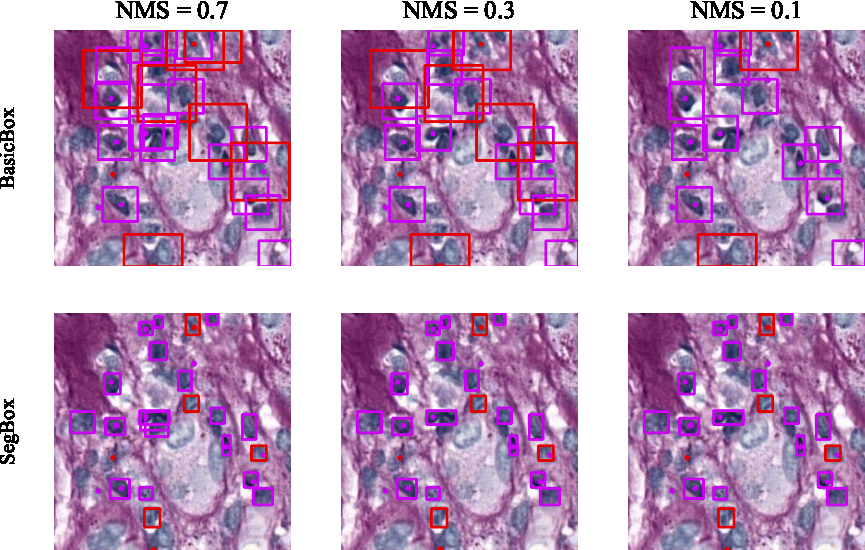
\includegraphics[width=\linewidth]{images/nms_comparison.pdf}
    \caption{Predictions of YOLO11 trained with BasicBox or SegBox labels using different NMS thresholds during inference. The confidence threshold of the predictions is set to 0.25, which maximizes the F1-score in all cases. The patches show bounding box predictions for lymphocytes (purple) and monocytes (red) with ground truth dot annotations marked in the same colors.}
    \label{fig:nms}
\end{figure}

\begin{table}
    \centering
    \begin{tabular}{lr|rrrrrr}
        \toprule
        Label Type & NMS & \multicolumn{3}{c}{Box-wise AP} & \multicolumn{3}{c}{Point-wise AP} \\
        & & L & M & \textbf{mAP} & L & M & \textbf{mAP} \\
        \midrule
        BasicBox & 0.7 & 0.785 & 0.525 & \textbf{0.655} & 0.707 & 0.418 & 0.562 \\
        BasicBox & 0.3 & 0.732 & 0.454 & 0.593 & 0.734 & 0.444 & \textbf{0.589} \\
        BasicBox & 0.1 & 0.599 & 0.348 & 0.473 & 0.609 & 0.341 & 0.475 \\
        \midrule
        SegBox & 0.7 & 0.559 & 0.296 & 0.427 & 0.610 & 0.320 & 0.465 \\
        SegBox & 0.3 & 0.569 & 0.301 & \textbf{0.435} & 0.671 & 0.411 & 0.541 \\
        SegBox & 0.1 & 0.570 & 0.301 & \textbf{0.435} & 0.676 & 0.423 & \textbf{0.549} \\
        \midrule
        MixedBox & 0.7 & 0.652 & 0.351 & \textbf{0.502} & 0.477 & 0.217 & 0.347 \\
        MixedBox & 0.3 & 0.641 & 0.347 & 0.494 & 0.617 & 0.308 & 0.462 \\
        MixedBox & 0.1 & 0.606 & 0.331 & 0.468 & 0.695 & 0.387 & \textbf{0.541} \\
        \bottomrule
    \end{tabular}
    \caption{Performance of models trained on patch size 512 with different bounding box types, using different NMS thresholds during inference. L: lymphocytes, M: monocytes, mAP: mean average precision.}
    \label{tab:exp_nms}
\end{table}

The effect of different NMS thresholds on the predictions for patch size 256 is shown in Figure~\ref{fig:nms}. Although SegBoxes and MixedBoxes performed slightly better on this patch size than on patch size 512, they still did not outperform BasicBoxes. I also evaluated the effect of different NMS thresholds on padded SegBox and MixedBox labels. However, their point-wise AP at lower NMS thresholds was eventually surpassed by the corresponding box types without padding.

\subsection{Immunohistochemistry Staining}
I also evaluated the performance of YOLO11 trained on IHC-stained patches, although IHC staining is not always available in practice and cannot be used for inference. The detection and classification of inflammatory cells should be easier with IHC because it distinctly stains both lymphocytes and monocytes, as shown in Figure~\ref{fig:ihc}, and the model no longer needs to rely solely on cell morphology. This experiment was conducted on patches of different sizes using BasicBox labels and an NMS threshold of 0.3. The NMS threshold was selected to maximize point-wise AP, on which it had a significant effect, particularly for lymphocyte detection.

The results in Table~\ref{tab:exp_ihc} show that IHC staining substantially improved monocyte detection, nearly doubling both box-wise and point-wise AP compared to models trained on PAS-stained patches. I initially intended to evaluate IHC staining with SegBox and MixedBox labels as well, and if these labels had improved performance, they could potentially have been used for model training on PAS-stained patches. However, I decided against this because these labels never outperformed BasicBoxes in previous PAS experiments. Additionally, SAM 2 segmented far fewer inflammatory cells in IHC-stained patches than in PAS-stained patches, as shown in Table~\ref{tab:boxes}, resulting in fewer SegBoxes and likely worse performance.

\begin{table}[h]
    \centering
    \begin{tabular}{lr|rrrrrr}
        \toprule
        Patch & Staining & \multicolumn{3}{c}{Box-wise AP} & \multicolumn{3}{c}{Point-wise AP} \\
        & & L & M & \textbf{mAP} & L & M & \textbf{mAP} \\
        \midrule
        512 & PAS & 0.732 & 0.454 & 0.593 & 0.734 & 0.444 & 0.589 \\
        \midrule
        512 & IHC & 0.686 & 0.823 & \textbf{0.755} & 0.774 & 0.780 & \textbf{0.777} \\
        256 & IHC & 0.681 & 0.815 & 0.748 & 0.735 & 0.775 & 0.755 \\
        128 & IHC & 0.693 & 0.777 & 0.735 & 0.723 & 0.757 & 0.740 \\
        \bottomrule
    \end{tabular}
    \caption{Performance of models trained on IHC-stained patches with BasicBoxes, using an NMS threshold of 0.3 during inference. L: lymphocytes, M: monocytes, mAP: mean average precision.}
    \label{tab:exp_ihc}
\end{table}

\begin{figure}
    \centering
    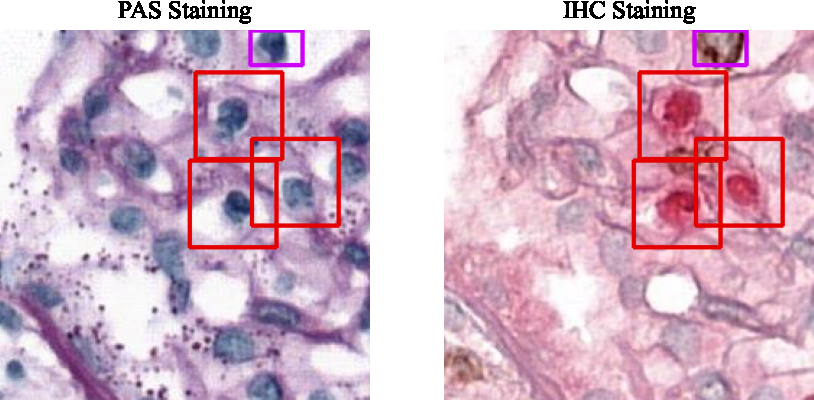
\includegraphics[width=\linewidth]{images/ihc_patch.pdf}
    \caption{Comparison of PAS and IHC staining with BasicBox labels for lymphocytes (purple) and monocytes (red). IHC produces a dark brown cytoplasmic staining of lymphocytes and a nuclear magenta staining of monocytes.}
    \label{fig:ihc}
\end{figure}


\section{Results}
I selected the best-performing YOLO11 model for inflammatory cell detection on PAS-stained images based on point-wise mAP, which evaluates detection quality directly against ground truth dot annotations. The highest point-wise mAP of 0.589 was achieved by the model trained for 100 epochs on patch size 512 with BasicBox labels, using an NMS threshold of 0.3 during inference. Examples of its detections are shown in Figure~\ref{fig:predictions} with a minimum prediction confidence threshold of 0.25, which approximately maximizes the F1-score of the model.

The selected model was trained using BasicBox labels over the proposed SegBox or MixedBox labels, which were generated from inflammatory cell segmentation masks predicted by SAM 2 and produced only mediocre results. The lack of satisfactory performance when using these bounding boxes suggests that the SAM 2 predictions are not sufficiently reliable to generate a better set of training labels. The performance of the baseline model was finally improved by applying a more aggressive NMS with a lower threshold. This also improved performance when using SegBoxes and MixedBoxes, but still not enough to outperform BasicBoxes.

Figure~\ref{fig:result_matrix} shows the confusion matrix of detections predicted by the selected model on the validation split, using a minimum confidence threshold of 0.25. The confusion matrix confirms that the model performs substantially better in lymphocyte detection than in monocyte detection, which was consistently observed in all experiments. It also shows that there is approximately the same number of false negative and false positive predictions across both classes and that the two cell types are not commonly misclassified.

\begin{figure}[t]
    \centering
    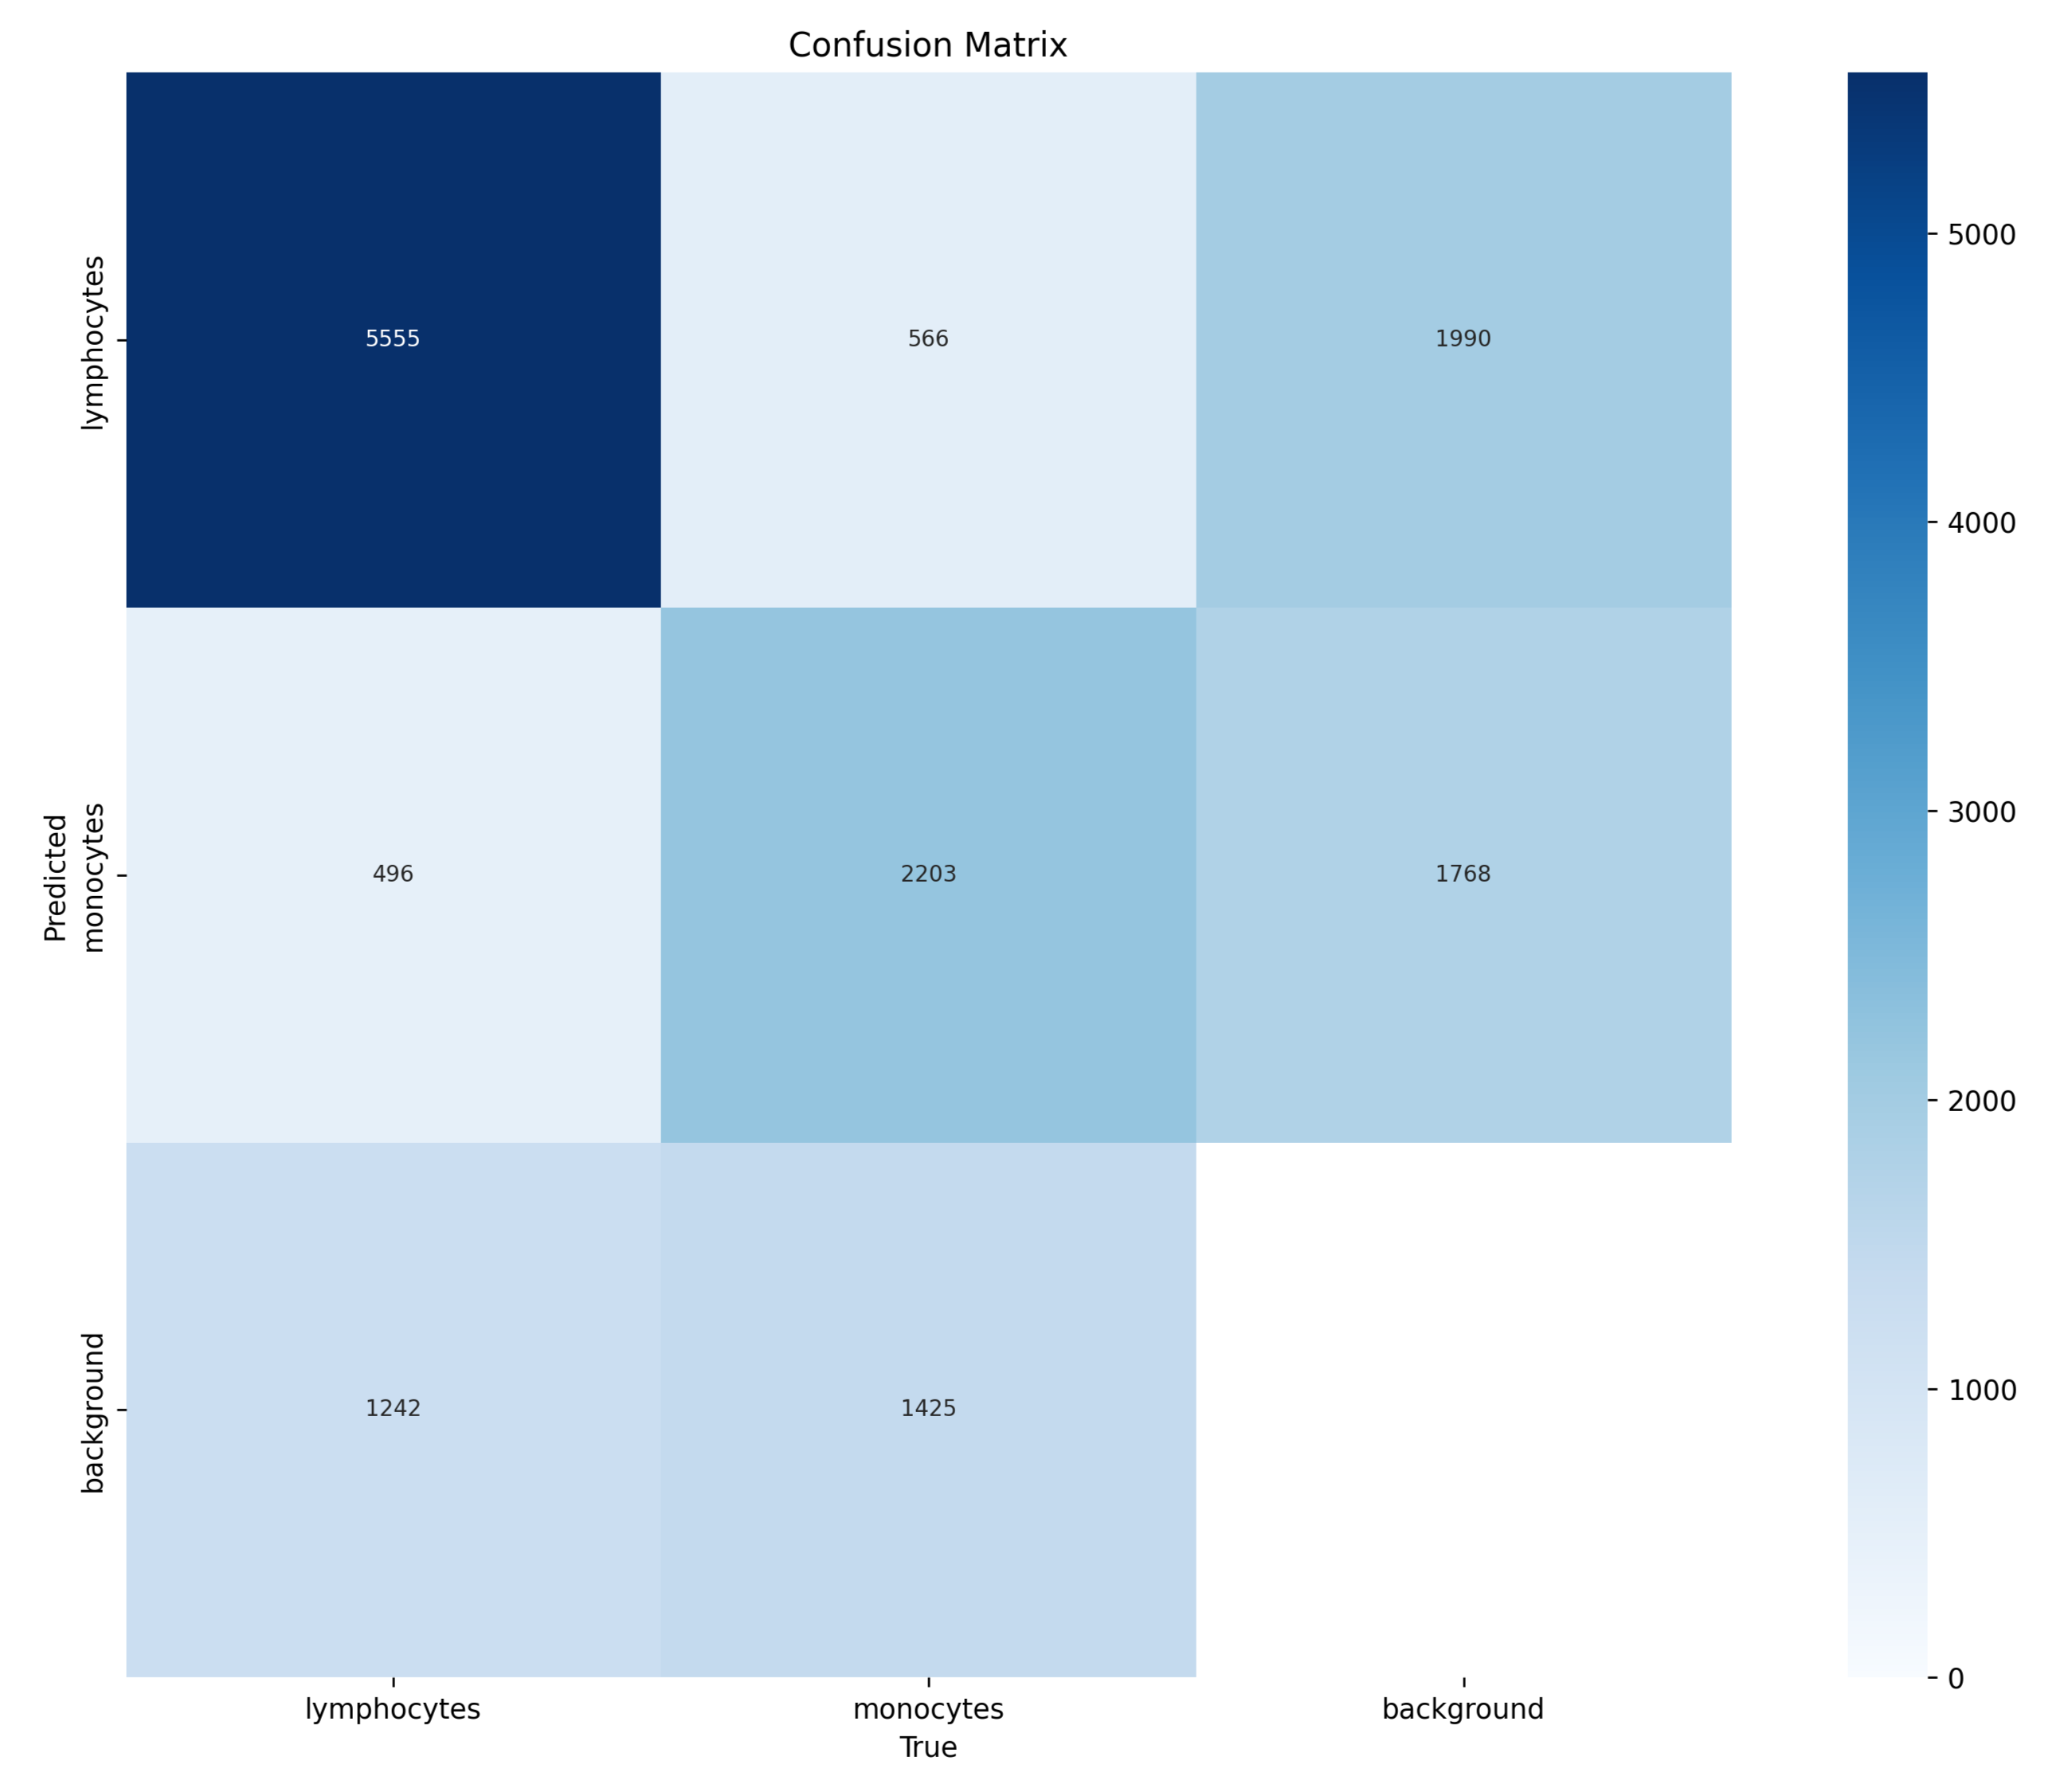
\includegraphics[width=\linewidth]{images/result_matrix.png}
    \caption{Confusion matrix of detections above a confidence threshold of 0.25 predicted by the selected YOLO11 model trained for 100 epochs on patch size 512 with BasicBox labels, using NMS threshold of 0.3 during inference.}
    \label{fig:result_matrix}
\end{figure}

\subsection{Challenge Submission}
All previous evaluations were performed at the patch level. To evaluate the selected model at the WSI level, I made a submission to the MONKEY Challenge~\cite{Studer2024}. The submission was evaluated on the hold-out validation set, which consists of nine PAS-stained WSIs, each accompanied by a tissue mask specifying the regions in which inflammatory cell detection should be performed.

Inference on WSIs was performed using a sliding window approach with a stride of 256 pixels, dividing each image into overlapping patches of size 512. Predicted bounding boxes located within three pixels of patch boundaries were removed to eliminate detections of partially visible cells that can be better detected in neighboring overlapping patches. After collecting predictions across all patches, an additional NMS was applied to remove duplicate detections introduced by the overlap.

The challenge evaluates detection quality using the Free Response Operating Characteristic (FROC) curve, which is an alternative to the ROC curve and plots recall on the y axis against the average number of false positives per $\mathrm{mm^2}$ on the x axis. An FROC score is derived by calculating recall at six predefined $\mathrm{FP/mm^2}$ thresholds: $\{10, 20, 50, 100, 200, 300\}$. I evaluated the FROC score throughout all previous experiments and observed that it behaves almost identically to point-wise AP, differing only in absolute scale. Consequently, the selected model, which achieved the highest AP, also achieved the highest FROC score. This similarity is expected because both metrics match predictions with ground truth annotations using the same procedure, and $\mathrm{FP/mm^2}$ captures a detection quality aspect similar to precision, which is used to calculate AP.

Table~\ref{tab:results} compares the selected model with the top five performing submissions on the MONKEY Challenge hold-out validation set. The selected model achieved results comparable to those of the other submissions, demonstrating that the proposed inflammatory cell detection approach is reasonable and delivers competitive performance. The selected model ranked fourth in mean FROC score and third in monocyte FROC score. Submissions from all teams performed substantially better in lymphocyte detection than in monocyte detection, confirming my observation that monocyte detection in the provided PAS-stained images is likely inherently more challenging.

\begin{table}
    \centering
    \begin{tabular}{lrrr}
        \toprule
        Algorithm & FROC -- L & FROC -- M & Mean FROC \\
        \midrule
        InstanSeg & 0.439 & 0.200 & 0.320 \\
        TIAKong~\cite{Lv2025} & 0.410 & 0.180 & 0.295 \\
        Aira Matrix~\cite{Deotale2025} & 0.384 & 0.132 & 0.258 \\
        ST Medical & 0.362 & 0.110 & 0.236 \\
        Amaranth & 0.338 & 0.126 & 0.232 \\
        \midrule
        YOLO11 + BasicBox & 0.347 & 0.144 & 0.246 \\
        \bottomrule
    \end{tabular}
    \caption{Performance of the selected model compared to the top five submissions to the MONKEY Challenge, evaluated using the FROC score on the hold-out validation set. L: lymphocytes, M: monocytes.}
    \label{tab:results}
\end{table}

\begin{figure}
    \centering
    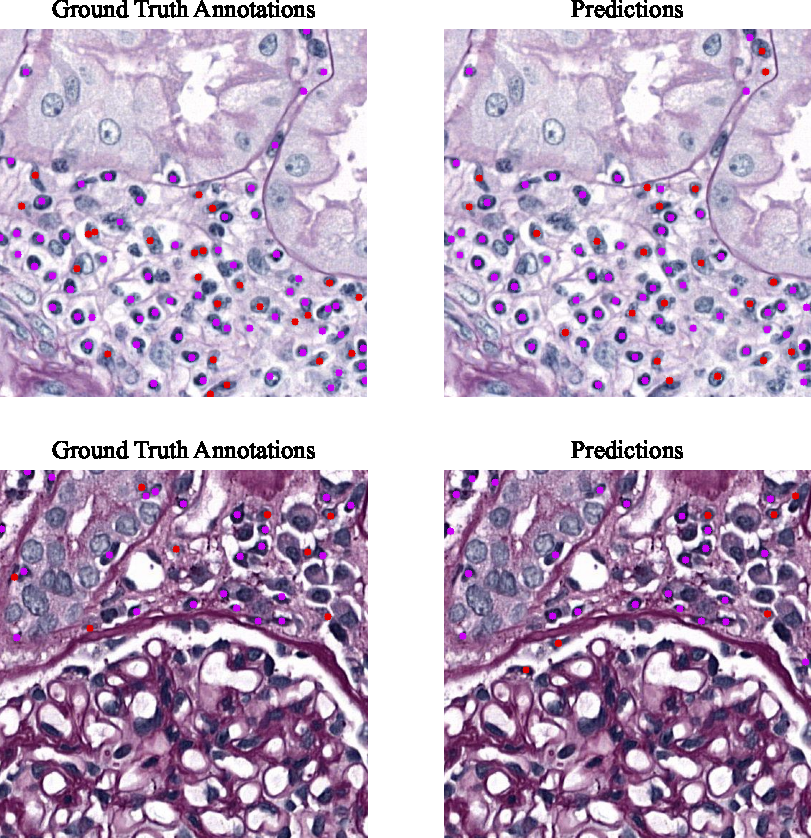
\includegraphics[width=\linewidth]{images/predictions.pdf}
    \caption{Comparison of ground truth dot annotations and detections predicted by the selected YOLO11 model on patches of size 512 with a confidence threshold of 0.25. The detections are represented by dots at the centers of predicted bounding boxes for lymphocytes (purple) and monocytes (red).}
    \label{fig:predictions}
\end{figure}



\chapter{Conclusion}
This thesis presents a deep learning approach for the automated detection of mononuclear inflammatory cells in kidney transplant biopsies, including their classification into lymphocytes and monocytes. These cells play a critical role in transplant rejection and their detection is essential for assessing the health of the transplanted organ and preventing potential failure. The proposed approach trains the object detection CNN YOLO11 on an annotated dataset provided for this task by the MONKEY Challenge.

Histological WSIs from the dataset were preprocessed into patches of fixed size, and provided dot annotations were converted into bounding box labels. A baseline model was trained on this preprocessed dataset using fixed-size BasicBox labels. Alternative labels generated from segmentation masks predicted by SAM 2 were tested, and several experiments were conducted to refine and compare them. Despite these efforts, the baseline model trained with BasicBox labels remained the most effective, with the only improvement obtained by lowering the NMS threshold.

The best-performing model was submitted to the MONKEY Challenge and evaluated on a hold-out validation set. It achieved competitive results and ranked fourth overall in mean FROC score for combined lymphocyte and monocyte detection and third for monocyte detection alone. The resulting performance is not sufficient to fully automate inflammatory cell detection during kidney transplant biopsy assessment, but the model could serve as a supportive tool for pathologists. In this context, high precision is likely more valuable than high recall, allowing pathologists to rely on model detections while manually reviewing only the remaining cells. The model could assist in the evaluation of more challenging, time-consuming, or borderline cases, helping confirm findings and reducing the risk of overlooking large numbers of inflammatory cells. 

The detection problem was approached by focusing primarily on generating higher-quality training labels. Although these efforts did not surpass the selected baseline, many alternative approaches remain viable. A more model-centric approach could explore different model architectures, perform thorough hyperparameter tuning, and identify the most suitable architecture for this task. Based on the results, an ensemble could be created either by combining multiple object detection models or by integrating models trained for different tasks, such as classification or segmentation, that would supplement the detection.

Another potential approach could utilize virtual staining~\cite{Bai2023} to generate IHC-stained images from PAS staining. The resulting IHC staining could then be used for more effective inference, as detecting inflammatory cells in IHC-stained images is substantially easier. These approaches are likely complementary and could be combined to further improve detection performance, making progress toward greater automation in the assessment of kidney transplant biopsies.
 % include `text.tex' from `text/' subdirectory

\appendix\appendixinit % do not remove these two commands

% \include{text/appendix} % include `appendix.tex' from `text/' subdirectory

\backmatter % do not remove this command

\begingroup
\sloppy
\printbibliography % print out the BibLaTeX-generated bibliography list
\endgroup

\chapter{Attachment Contents}
% Contents of the attachment

    \dirtree{%
		.1 /.
		.2 LICENSE.txt\DTcomment{license agreement}.
		.2 metrics.xlsx\DTcomment{comprehensive table of evaluated metrics}.
        .2 model.pt\DTcomment{weights of the best-performing YOLO11 model}.
		.2 README.md\DTcomment{overview of the attachment contents}.
		.2 requirements.txt\DTcomment{Python package dependencies}.
		.2 data.
        .3 raw\DTcomment{sample WSI training data}.
		.2 inference-docker\DTcomment{Docker setup for challenge submission}.
		.2 notebooks\DTcomment{Jupyter notebooks for data exploration}.
		.2 scripts\DTcomment{scripts for preprocessing, training, and evaluation}.
        .2 thesis.
        .3 src\DTcomment{\LaTeX{} source files}.
        .3 thesis.pdf\DTcomment{compiled thesis PDF}.
		.2 yolo\DTcomment{training logs and visualizations of evaluated metrics}.
	}
 % include `medium.tex' from `text/' subdirectory

\end{document}
